\documentclass{uulm-assignment}

\usepackage{import}
\usepackage{tabularx}
\usepackage{listings}
\usepackage{todonotes}
\usepackage{graphicx}
\usepackage{siunitx}
\usepackage{placeins}
\usepackage{tikz}
\usepackage{tikz-uml}
\setboolean{showsolutions}{false}

\ifthenelse{\boolean{showsolutions}}{
\newcommand\mitloesung{1}%
}{
\newcommand\mitloesung{0}%
}


% Für Korrektur-Kommentare in roten Boxen:
\newcommand{\flo}[1]{
    \fcolorbox{purple}{pink}{\sffamily\scriptsize\bfseries\textcolor{black}{Flo:}} {\sffamily\bfseries\textcolor{purple}{#1}}
}

% Entnommen und angepasst von https://github.com/SoPra-Team-10
\newcommand{\Fachwissen}[7] {
		\begin{tabular}{|p{2,25cm}|p{12cm}|}
			\hline
			\textbf{Begriff} & \textbf{#1} \\
			\hline
			\textbf{Beschreibung} & #2 \\ 
			\hline
			\textbf{Ist-ein} & #3 \\
			\hline
			\textbf{Kann-sein} & #4 \\ 
			\hline
			\textbf{Aspekt} & #5 \\ 
			\hline
			\textbf{Bemerkung} & #6 \\ 
			\hline
			\textbf{Beispiel} & #7 \\
			\hline
		\end{tabular}
}

\newcommand{\FachwissenSyn}[8] {
		\begin{tabular}{|p{2,25cm}|p{12cm}|}
			\hline
			\textbf{Begriff} & \textbf{#1} \\
			\hline
			\textbf{Beschreibung} & #2 \\ 
			\hline
			\textbf{Ist-ein} & #3 \\
			\hline
			\textbf{Kann-sein} & #4 \\ 
			\hline
			\textbf{Aspekt} & #5 \\ 
			\hline
			\textbf{Bemerkung} & #6 \\ 
			\hline
			\textbf{Beispiel} & #7 \\
			\hline
			\textbf{Synonym} & #8 \\
			\hline
		\end{tabular}
}



\hypersetup{colorlinks=false,urlcolor=uulm-in}

\faculty{Institut für Softwaretechnik und Programmiersprachen\hspace{0.05cm}}
\course{Softwaregrundprojekt}
\semester{\hspace{0.05cm}WiSe 2019/20}
\supervisor{\textbf{} \hspace{7.9cm} Prof. Dr. Matthias Tichy, Florian Ege, Dennis Jehle}
 
%\assignmentdeadline{}         % Abgabedatum: XYZ
%\assignmentduration{15 Minuten} % Bearbeitungsdauer: XYZ
% \studentdata                      % Name & Matrikelnummer Feld

\assignmenttype{}
\assignmentno{}
\title{Pflichtenheft Team 17}

\begin{document}

\maketitle

\tableofcontents

\clearpage
\section{Kontextanalyse}
\subsection{Einleitung}
In diesem Projekt soll ein rundenbasiertes Taktik-Multiplayer-Spiel für maximal zwei Spieler entwickelt werden. Das Spiel handelt im James Bond Universum. 
Der Schauplatz des Spiels ist ein Casino. In diesem Casiono befinden sich zwielichtige Gestalten verschiedenster Herkunft, zwei Spionage-Teams und vor allem die weiße Katze des Bösewichts Ernst Stavro Blofeld. Die Katze hat ihr Diamanthalsband verloren und versucht dieses wiederzufinden.
Die Spione hoffen, wenn sie das Diamanthalsband finden, die Gunst des Kätzchens und damit die Gunst der zwielichtigen Organisation, welcher das Kätzchen angehört, zu gewinnen.
Die Spieler kontrollieren jeweils ein Team von Agenten. Am Ende gewinnt derjenige, der es schafft das Diamanthalsband aufzuspüren.


\subsection{Motivation}
Am 3.April 2020 wird der 25. von \textit{Eon Productions} produzierte James Bond Film mit dem Titel \textit{No Time to Die} veröffentlicht. Um dieses Jubiläum zu feiern, soll ein Spiel im James Bond Universum entwickelt werden.
Das Spiel soll den Spirit von James Bond wiederspiegeln mit abgefahrenen Bösewichten, spannenden Geschichten und vor allem jeder Menge Spionage!\\
Die Entscheidung für das Medium Videospiel fiel, da dieses vor allem bei jungen Menschen beliebter denn je ist. Das Spiel soll sich vor allem an eine junge Zielgruppe richten und diesen ein cooles Spielerlebnis bieten.\\

Der Auftraggeber erhält hierbei die Rechte an einem Spiel in einem der größten Filmuniversen. Dadurch wird eine große Zielgruppe angesprochen und da es sich bei dem Spiel um ein Mehrspieler-Spiel handelt, verbreitet sich dieses schnell.


\subsection{Vision}
\textit{No Time to Spy} soll ein ein 2D-Spiel werden. Die verschiedenen Charaktere im Spiel erhalten jeweils ein individuelles Aussehen. Das Spiel soll also nicht nur durch spannendes Spieldesign sondern auch gutes Aussehen glänzen. Der Spieler soll die Möglichkeit haben viele der Aktionen, welche ihm selbst einfallen, im Spiel umzusetzen. Dazu gehört im Casino spielen zu können, einen Cocktail zu trinken, um andere Spieler abzulenken, diese mit einem Cocktail zu übergießen und vieles mehr.\\
Das Spiel soll zudem viele verschiedene Charaktere, Eigenschaften und Gadgets enthalten und so eine Tiefe bieten, dass auch bei häufigen Spielen keine Langeweile entsteht. Das Spiel wird mehr als 10 verschiedene Eigenschaften, beinahe 20 verschiedene Gadgets und mehr als 25 verschiedene Charaktere aus dem James Bond Universum enthalten. \\
Trotz der Komplexität des Spiels soll auch Anfängern oder Neulingen in James Bond Universum ein gutes Spielerlebnis geboten werden. Ermöglicht wird dies durch ausführliche Beschreibungen der Eigenschaften und Charaktere und einer sinnvollen Hilfsfunktion im Spiel.\\
Um auch alleine Spielen zu können, wird das Spiel einen KI-Gegner beinhalten. Dieser kann auf verschiedene Schwierigkeiten eingestellt werden, so dass jeder Spieler ein für sich angenehmes Spielerlebnis geboten bekommt.\\
Um zu einem abwechslungsreichen Spielerlebnis beizutragen, enthält das Spiel einen Charakter- und Szenarioeditor. In diesem kann das Spielfeld und die eigene Gruppe an Agenten bearbeitet werden. 

\subsection{Projektkontext}
Das Spiel \textit{No Time to Spy} wird zunächst im Rahmen des Software-Grundprojekts an der Universität Ulm im Wintersemester 2019/2020 und Sommersemester 2020 entwickelt.
Eine mögliche Weiterentwicklung nach dem Software-Grundprojekt ist nicht ausgeschlossen. Insbesondere wird das Spiel nach Abschluss des Projekts unter einer Open-Source-Lizenz zur Verfügung gestellt, so dass auch dritte daran weiterentwickeln können.\\

Im Rahmen der Entwicklung wird ein Client entstehen. Dieser bietet eine graphische Benutzeroberfläche mit welcher der Spieler interagiert. Außerdem kann der Benutzer einen Charakter- und Leveleditor verwenden, dieser ist ebenfalls teil des Projekts und bietet dem Benutzer eine graphische Oberfläche.\\
Es wird ein Server implementiert der verschiedene Spielpartien verwaltet, auf Regelverstöße achtet und den Ablauf des Spiels kontrolliert. Außerdem wird eine KI entwickelt die am Spiel teilnehmen kann.


\clearpage
\section{Fachwissen}
Im Folgenden werden Abkürzungen und domänenspezifische Begriffe, welche für das Verständnis dieses Dokuments wichtig sind, definiert.

\todo[inline] {Fachwissen vervollständigen}

\Fachwissen{Angriff}
{TODO}
{-}
{-}
{-}
{-}
{-}

\Fachwissen{Balancing}
{Unter Balancing versteht man das Verändern von Spielparametern mit dem Ziel mehr Chancengleichheit zwischen den Spielern herzustellen.}
{Instrument der Spielgestaltung.}
{Stärken bzw. Schwächen von Spielfiguren und Items.}
{Die Veränderung der Spielparameter erfolgt über den Editor.}
{-}
{Erhöhung der Health-Points des Charakters \glqq James Bond \grqq.}

\FachwissenSyn{Charakter}
{Eine Figur aus den James-Bond Filmen oder Romanen, die durch eine Einheit auf dem Raster der Spielfelder repräsentiert wird.}
{Bewegliche Einheit.}
{Player-Character (PC), Non-Player-Charakter (NPC).}
{Besitzt einen Namen, Eigenschaften, Gadgets im Inventar, Vorrat an Casino-Spielchips, Health Points, Intelligence Points, eine Position auf dem Spielfeld und ist einer Fraktion zugehörig oder ein NPC.}
{Der Begriff \glqq Charakter\grqq bezeichnet eine Person, die in der Welt des Spiels im Casino herumläuft.}
{Dr. Madelein Swann ist ein zur Auswahl stehender Charakter.}
{Spielfigur}

\Fachwissen{Client}
{Der Client ist diejenige Spielkomponente, welche dem Nutzer eine grafisches Oberfläche bereitstellt. Mit dieser hat der Nutzer die Möglichkeit sich mit einem Server zu verbinden und einer Partie als Spieler oder Zuschauer beizutreten. Über die grafische Oberfläche wird während einer Partie das Spiel visualisiert und mit dem Spieler interagiert. }
{-}
{-}
{Notwendig zum Spielen von \glqq No Time To Spy\grqq.}
{Der Begriff Client bezeichnet nicht die Person welches die Anwendung bedient, sondern auf die Softwarekomponente selbst.}
{-}

\FachwissenSyn{Continous Integration}
{Continous Integration beschreibt den Vorgang des permanenten Zusammenfügens aller Komponenten während des Entwicklungsprozesses. Insbesondere bei der Entwicklung in Teams bedeutet dies, dass die Änderungen der einzelnen Personen sehr früh wieder zusammengeführt werden, sodass eventuelle Probleme in der Abstimmung frühzeitig erkannt und beseitigt werden können.}
{Prozess der Softwareentwicklung}
{-}
{-}
{-}
{-}
{Kontinuierliche Integration, Fortlaufende Integration}

\Fachwissen{C++}
{C++ ist eine von der \glqq International Organization for Standardization\grqq in verschiedenen Standards genormte Programmiersprache.}
{Programmiersprache}
{-}
{C++ ermöglicht imperative und objektorientierte Programmierung.}
{-}
{C++17 ist ein möglicher Standardisierung von C++.}

\Fachwissen{Docker-Container}
{Ein Docker-Container ist eine Form der Virtualisierung und enthält eine Anwendung sowie die zur Laufzeit notwendigen Ressourcen. Um die Anwendung auf einem System auszuführen wird also lediglich die Container-Engine von Docker benötigt, sämtliche anderen Abhängigkeiten werden vom Container aufgelöst.}
{Virtualisierungstool}
{-}
{-}
{Die Serverkomponente des Spiels wird in einem Docker-Container realisiert um plattformunabhängiger entwickeln zu können.}
{-}

\FachwissenSyn{Editor}
{Stellt dem Nutzer eine grafische Oberfläche bereit, mit welcher die Spielkonfiguration angepasst werden kann. }
{-}
{-}
{Ermöglicht dem Nutzer eigene Level zu erstellen.}
{-}
{-}
{Konfigurator, Level-Editor}

\Fachwissen{Fraktion}
{TODO}
{-}
{-}
{-}
{-}
{-}

\FachwissenSyn{Geheiminformation}
{TODO}
{-}
{-}
{-}
{-}
{-}
{Geheimnis}

\FachwissenSyn{Health-Points (HP)}
{Unter Health-Points versteht man die Anzahl der Lebenspunkte, die eine Spielfigur besitzt. Diese wird in der Spielkonfiguration festgelegt. Während einer Partie kann die Spielfigur von anderen Spielfiguren angegriffen werden und Schaden nehmen. Der erlittene Schaden wird dann von den noch vorhanden Lebenspunkten abgezogen.}
{-}
{-}
{Sinken die Health-Points unter einen Punkt, so muss die Spielfigur exfiltriert werden.}
{-}
{Die Spielfigur \glqq James Bond\grqq besitzt 100 HP.}
{Lebenspunkte}

\Fachwissen{Intelligence Points (IP)}
{Intelligence Points repräsentieren, wie gut ein Charakter beim Spionieren war. Für jedes in Erfahrung gebrachte Geheimnis bekommt der Charakter eine entsprechende Anzahl an Intelligence Points.}
{Elementarer Spielbestandteil.}
{-}
{Intelligence Points sind die primäre Metrik zur Bestimmung des Siegers.}
{-}
{-}

\Fachwissen{Künstliche Intelligenz (KI)}
{Die Künstliche Intelligenz definiert den Algorithmus bzw. die Regeln, nach welcher der KI-Client seine Aktionen im Spielverlauf auswählt.}
{-}
{-}
{Notwendig für Spiele gegen einen Computergegner.}
{Der Begriff \glqq Künstliche Intelligenz\grqq beschreibt lediglich die Logik, nach welcher die Aktionen ausgewählt werden. Die Implementierung erfolgt im KI-Client.}
{-}

\FachwissenSyn{KI-Client}
{Der KI-Client interagiert mit dem Server wie ein normaler Client, mit der Besonderheit, dass er das menschliche Verhalten lediglich simuliert und nicht von einem Menschen gesteuert wird. In Folge dessen besitzt der KI-Client keine graphische Benutzeroberfläche. }
{-}
{-}
{Notwendig für Spiele gegen einen Computergegner.}
{Der Begriff KI-Client beschreibt die Implementierung der Logik einer künstlichen Intelligenz.}
{-}
{Computergegner, Bot}

\Fachwissen{Level}
{TODO}
{-}
{-}
{-}
{-}
{-}

\Fachwissen{Merge-Request}
{Unter einem Merge-Request wird eine Anfrage zum \glqq mergen \grqq des Standes eines Entwicklungszweiges in den Hauptzweig verstanden. Ziel ist es dabei, dass neue Features auf eigenen Entwicklungszweigen implementiert werden und erst nach eingehender Prüfung in den Hauptzweig übernommen.}
{Feature der Versionsverwaltungssoftware Git.}
{-}
{-}
{Zentraler Bestandteil des Feature-Branch-Workflows.}
{-}

\Fachwissen{Monkey-Testing}
{Unter Monkey-Testing wird eine spezielle Form des Softwaretestens verstanden, bei welcher zufällige Nutzereingaben simuliert werden. Ziel ist es dabei sicherzustellen, dass die Anwendung in keinem Fall abstürzt.}
{Negativtest.}
{-}
{-}
{Wird in Ergänzung zu den Unit-Tests verwendet.}
{-}

\Fachwissen{Nicht-Spieler Charakter (NPC)}
{Unter einem NPC wird eine Spielfigur verstanden, welche von keinem der beiden Spieler gesteuert wird. Für die Spieler ist es dabei lediglich ersichtlich, dass der Charakter nicht zu ihrer Fraktion gehört, allerdings nicht, ob er zur gegnerischen Fraktion gehört. Die Aktionen der Spielfiguren werden dabei vom Server gesteuert, allerdings ohne auf ein Spielziel hinzuwirken.}
{Spielfigur}
{-}
{-}
{Die Spielfigur \glqq James Bond\grqq wird vom Server gesteuert und ist somit ein NPC.}

\Fachwissen{Nutzer}
{Ein Nutzer ist eine Person, welche über den Client mit dem Spiel  \glqq No Time To Spy\grqq interagiert. Diese Interaktion kann durch Bedienen des Konfigurators, Spielen des Spiels oder Beobachten einer laufenden Partie erfolgen.}
{-}
{Spieler, Zuschauer}
{-}
{-}
{Der Nutzer \glqq Max Mustermann\grqq interagiert mit dem Client.}

\Fachwissen{Partie}
{Unter einer Partie versteht man die Gesamtheit eines Spiels. Diese beginnt mit der Drafting-Phase und endet mit der Feststellung des Gewinners.}
{-}
{-}
{Zu Beginn der Partie wird die Partiekonfiguration vom Server geladen.}
{-}
{-}

\Fachwissen{Partie-Konfiguration}
{Die Einstellungen für eine Partie werden in einer separaten Konfigurationsdatei im JSON-Format gespeichert. }
{-}
{-}
{Enthält Zeitlimits für die Bewegungs- und Aktionsphase, Wahrscheinlichkeiten von Spielereignissen, Anzahl der Runden bis zum Wechsel in den Modus für überlange Partien und das zu spielende Szenario.}
{-}
{-}

\Fachwissen{Runde}
{TODO}
{-}
{-}
{-}
{-}
{-}

\Fachwissen{Server}
{Der Server ist die zentrale Komponente des Spiels, in welcher die gesamte Spiellogik implementiert ist und über welche die Clients miteinander kommunizieren. Der Server stellt eine Kommandozeilenanwendung dar und besitzt keine grafische Oberfläche. Für die Kommunikation zwischen Server und Clients werden Nachrichten im JSON-Format über das WebSocket-Protokoll ausgetauscht.}
{-}
{-}
{Zuständig für die Kommunikation mit Clients und die Verwaltung der Spielpartien mitsamt der gesamten Spiellogik.}
{Der Server besitzt keine grafische Oberfläche, sondern lediglich ein Kommandozeileninterface.}
{-}

\Fachwissen{Spieler}
{Ein Spieler ist ein Nutzer, welcher sich in einer Partie des Spiels \glqq No Time To Spy\grqq gegen einen anderen Spieler befindet.}
{Nutzer}
{-}
{Menschlicher Spieler, KI-Client}
{-}
{-}

\Fachwissen{Spielfeld}
{Das Spielfeld beschreibt die festgelegte Fläche, auf welcher sich die Spielfiguren bewegen.}
{-}
{-}
{-}
{-}
{-}

\FachwissenSyn{Unit-Test}
{Unit-Tests werden in der Softwareentwicklung verwendet, um einzelne Module gezielt und automatisiert Funktionstests unterziehen zu können.}
{Testvariante in der Softwareentwicklung}
{-}
{-}
{Werden eingesetzt um die Funktionalität der einzelnen Module des Spiels zu überprüfen.}
{Google Test ist ein Framework für Unit-Tests mit C++.}
{Modultest, Komponententest}

\Fachwissen{WebSocket-Protokoll}
{Das WebSocket-Protokoll ist ein Netzwerkprotokoll, welches auf TCP basiert und für eine bidirektionale Verbindung genutzt werden kann.}
{Netzwerkprotokoll}
{-}
{-}
{-}
{-}

\Fachwissen{Zufall}
{Unter Zufall wird in diesem Dokument das Ziehen aus einer Normalverteilung verstanden.}
{-}
{-}
{Der Eintritt von Ereignissen innerhalb einer Runde wird vom Zufall bestimmt.}
{-}
{-}

\Fachwissen{Zug}
{TODO}
{-}
{-}
{-}
{-}
{-}

\Fachwissen{Zuschauer}
{Ein Zuschauer ist ein Nutzer, welcher eine Partie des Spiels \glqq{}No Time To Spy\grqq{} beobachtet. Dabei kann er das gesamte Spielfeld einsehen, allerdings im Gegensatz zu den Spielern keinen Einfluss auf das Spielgeschehen nehmen. Der Zuschauer besitzt dabei die Möglichkeit im Gegensatz zu den Spielern das gesamte Spielfeld einsehen zu können, kann allerdings auch auswählen, das Spiel aus Sicht einer der beiden Spieler zu verfolgen.}
{Nutzer}
{-}
{-}
{-}
{Der Nutzer \glqq Max Mustermann\grqq beobachtet die laufende Spielpartie als Zuschauer.}



\clearpage
\section{Domänenmodell}
\FloatBarrier
\begin{figure}[h]
    \centering
    \includegraphics[width=\textwidth]{Meilenstein01/domainmodel.pdf}
    \caption{Domänenmodell}
\end{figure}

\FloatBarrier

\begin{figure}[h]
    \centering
    \includegraphics[width=\textwidth]{Meilenstein01/fields.pdf}
    \caption{Domänenmodell: Feld}
\end{figure}
\FloatBarrier


\begin{figure}[h]
    \centering
    \includegraphics[width=\textwidth]{Meilenstein01/gadgets.pdf}
    \caption{Domänenmodell: Gadget}
\end{figure}
\FloatBarrier



\clearpage
\section{Spezifische Anforderungen}
Dieser Abschnitt enthält alle spezifischen Anforderungen des Systems. Er bietet eine detaillierte
Beschreibung des Systems und seiner Funktionen.


\subsection{Akteure}
%Hier kommen die Akteure rein

\begin{tabularx}{16cm}{l|X}
	\textbf{Akteur} & \textbf{Server} \\
	\hline
	Rolle & Zentrale Software-Einheit zur Kommunikation mit den Clients.\\ 
	\hline
	Aufgabe & Der Server ist Vermittler in der Kommunikation zwischen den Clients. Er geht auf Anfrage Verbindungen mit Clients ein und kann diese auch wieder beenden. Während ein Client mit dem Server verbunden ist, bearbeitet und validiert der Server alle Anfragen des Clients und sorgt dafür, dass der Client alle notwendigen Informationen zum aktuellen Stand erhält.\\ 
\end{tabularx}

\begin{tabularx}{16cm}{l|X}
	\textbf{Akteur} & \textbf{Client} \\
	\hline
	Rolle & Lokale Software-Einheit zur Kommunikation mit dem Server \\ 
	\hline
	Aufgabe & Da Clients nicht direkt miteinander kommunizieren können, kommuniziert der Client mit einem Server. Der Client kann eine Verbindung zum Server auf- und auch wieder abbauen. Ein verbundener Client kann Informationen weitergeben, anfragen und erhalten.\\ 
\end{tabularx}

\begin{tabularx}{16cm}{l|X}
	\textbf{Akteur} & \textbf{Benutzer-Client} \\
	\hline
	Rolle & Client, der von einem Menschen bedient wird.\\ 
	\hline
	Aufgabe & Der Benutzer-Client stellt eine graphische Oberfläche zur Bedienung zur Verfügung. Er ermöglicht die Bedienung des Editors und die Teilnahme an einer Spielpartie.\\ 
\end{tabularx}

\begin{tabularx}{16cm}{l|X}
	\textbf{Akteur} & \textbf{KI-Client} \\
	\hline
	Rolle & Client, der von einem Computer gesteuert wird.\\ 
	\hline
	Aufgabe & Der KI-Client kann von einem Benutzer-Client als Spieler zur Spielpartie hinzugefügt werden und benutzt keine graphische Oberfläche.\\ 
\end{tabularx}

\begin{tabularx}{16cm}{l|X}
	\textbf{Akteur} & \textbf{Teilnehmer} \\
	\hline
	Rolle & Alle Akteure, die an einer Spielpartie teilnehmen.\\ 
	\hline
	Aufgabe & Teilnehmer erhalten Informationen zur Spielpartie vom Server und können die Spielpartie jederzeit wieder verlassen.\\ 
\end{tabularx}

\begin{tabularx}{16cm}{l|X}
	\textbf{Akteur} & \textbf{Zuschauer} \\
	\hline
	Rolle & Benutzer-Client, der passiv an einer Spielpartie teilnimmt.\\ 
	\hline
	Aufgabe & Über die graphische Oberfläche des Benutzer-Clients, kann der Benutzer das laufende Spiel beobachten, aber nicht eingreifen. \\ 
\end{tabularx}

\begin{tabularx}{16cm}{l|X}
	\textbf{Akteur} & \textbf{Spieler} \\
	\hline
	Rolle & Client, der aktiv an einer Spielpartei teilnimmt.\\ 
	\hline
	Aufgabe & Wenn ein Spieler an der Reihe ist, führt er durch Steuerung seiner Charaktere valide Spielzüge aus und informiert den Server über seine Aktionen. Ziel des Spielers ist es, die Spielpartie zu gewinnen.\\ 
\end{tabularx}

\begin{tabularx}{16cm}{l|X}
	\textbf{Akteur} & \textbf{Benutzer-Spieler} \\
	\hline
	Rolle & Spieler, der ein Benutzer-Client ist.\\ 
	\hline
	Aufgabe & Ein Benutzer-Spieler spielt die Spielpartie über die graphische Oberfläche.\\ 
\end{tabularx}

\begin{tabularx}{16cm}{l|X}
	\textbf{Akteur} & \textbf{KI-Spieler} \\
	\hline
	Rolle & Spieler, der ein KI-Client ist.\\ 
	\hline
	Aufgabe & Ein KI-Spieler spielt die Spielpartie unter Verwendung von künstlicher Intelligenz.\\ 
\end{tabularx}

\begin{tabularx}{16cm}{l|X}
	\textbf{Akteur} & \textbf{NPC} \\
	\hline
	Rolle & Charakter in einer Spielpartie, der von keinem Spieler gesteuert werden kann.\\ 
	\hline
	Aufgabe & NPCs sind Charaktere, die vom Server gesteuert werden. Der Server informiert die Teilnehmer über die Spielzüge der NPCs.\\ 
\end{tabularx}

\begin{tabularx}{16cm}{l|X}
	\textbf{Akteur} & \textbf{Auftraggeber} \\
	\hline
	Rolle & Florian Ege, stellvertretend für das Institut für Softwaretechnik und Programmiersprachen\\ 
	\hline
	Aufgabe & Gibt die Anforderungen für \glqq No Time To Spy\grqq vor und nimmt das fertige Produkt ab.\\ 
\end{tabularx}

\begin{tabularx}{16cm}{l|X}
	\textbf{Akteur} & \textbf{Vertreter des Auftraggebers} \\
	\hline
	Rolle & Tutor Ismail Temel\\ 
	\hline
	Aufgabe & Dient als Vermittler zwischen Entwicklern und Auftraggeber.\\ 
\end{tabularx}

\begin{tabularx}{16cm}{l|X}
\textbf{Akteur} & \textbf{Entwickler} \\
\hline
Rolle & SoPra-Team-17: Dominik Authaler, Lukas Bleile, Marco Deuscher, Jonas Otto, Carolin Schindler, Dominik Tabib Khoie\\ 
\hline
Aufgabe & Agile Entwicklung von \glqq No Time To Spy\grqq nach den Anforderungen des Auftraggebers.\\ 
\end{tabularx}


\clearpage
\subsection{Funktionale Anforderungen}

Dieser Abschnitt enthält alle Anforderungen, die die grundlegenden Aktionen des Softwaresystems
spezifizieren.

\subsubsection{Server}

\begin{tabularx}{16cm}{l|X}
\textbf{ID} & \textbf{FA-S} \\
\hline
TITEL: & Partie Konfiguration \\
\hline
BESCHREIBUNG: & Der Server muss beim Start die Partie Konfiguration aus einer Datei lesen. \\
\hline
BEGRÜNDUNG: & Die Konfiguration soll für das Balancing des Spiels einfach angepasst werden können. \\
\hline
ABHÄNGIGKEITEN: & \\
\end{tabularx}

\begin{tabularx}{16cm}{l|X}
\textbf{ID} & \textbf{FA-S} \\
\hline
TITEL: & Szenario Konfiguration \\
\hline
BESCHREIBUNG: & Der Server muss beim Start die Szenario Konfiguration (Spielfeld) aus einer Datei lesen. \\
\hline
BEGRÜNDUNG: & Das Spielfeld soll veräderbar sein. \\
\hline
ABHÄNGIGKEITEN: & \\
\end{tabularx}

\begin{tabularx}{16cm}{l|X}
\textbf{ID} & \textbf{FA-S} \\
\hline
TITEL: & Charakter Konfiguration \\
\hline
BESCHREIBUNG: & Der Server muss beim Start die Konfiguration der Charaktere aus einer Datei lesen. \\
\hline
BEGRÜNDUNG: & \\
\hline
ABHÄNGIGKEITEN: & \\
\end{tabularx}

\begin{tabularx}{16cm}{l|X}
\textbf{ID} & \textbf{FA-S} \\
\hline
TITEL: & Client Verbindung \\
\hline
BESCHREIBUNG: & Der Server muss mittels Websockets über TCP eine Verbindung mit dem Client halten.
Die Verbindung wird vom Client initiiert. Bei Verbindungsabbruch muss die Verbindung wiederhergestellt werden. \\
\hline
BEGRÜNDUNG: & Integrale Funktionalität des Servers \\
\hline
ABHÄNGIGKEITEN: & \\
\end{tabularx}

\begin{tabularx}{16cm}{l|X}
\textbf{ID} & \textbf{FA-S} \\
\hline
TITEL: & Zuschauer \\
\hline
BESCHREIBUNG: & Ein Client kann sich als Zuschauer verbinden, bekommt also Updates über den Spielzustand, kann aber nicht aktiv am Spiel teilnehmen. \\
\hline
BEGRÜNDUNG: & \\
\hline
ABHÄNGIGKEITEN: & \\
\end{tabularx}

\begin{tabularx}{16cm}{l|X}
\textbf{ID} & \textbf{FA-S} \\
\hline
TITEL: & Client Timeout \\
\hline
BESCHREIBUNG: & \\
\hline
BEGRÜNDUNG: & \\
\hline
ABHÄNGIGKEITEN: & \\
\end{tabularx}

\begin{tabularx}{16cm}{l|X}
\textbf{ID} & \textbf{FA-S} \\
\hline
TITEL: & Verspätete Nachrichten \\
\hline
BESCHREIBUNG: & \\
\hline
BEGRÜNDUNG: & \\
\hline
ABHÄNGIGKEITEN: & \\
\end{tabularx}

\begin{tabularx}{16cm}{l|X}
\textbf{ID} & \textbf{FA-S} \\
\hline
TITEL: & Spiel Durchführung \\
\hline
BESCHREIBUNG: & \\
\hline
BEGRÜNDUNG: & \\
\hline
ABHÄNGIGKEITEN: & \\
\end{tabularx}

\begin{tabularx}{16cm}{l|X}
\textbf{ID} & \textbf{FA-S} \\
\hline
TITEL: & Spielpause \\
\hline
BESCHREIBUNG: & \\
\hline
BEGRÜNDUNG: & \\
\hline
ABHÄNGIGKEITEN: & \\
\end{tabularx}

\begin{tabularx}{16cm}{l|X}
\textbf{ID} & \textbf{FA-S} \\
\hline
TITEL: & Erkennung von Regelverstößen \\
\hline
BESCHREIBUNG: & \\
\hline
BEGRÜNDUNG: & \\
\hline
ABHÄNGIGKEITEN: & \\
\end{tabularx}

\begin{tabularx}{16cm}{l|X}
\textbf{ID} & \textbf{FA-S} \\
\hline
TITEL: & Senden des Spielzustands \\
\hline
BESCHREIBUNG: & \\
\hline
BEGRÜNDUNG: & \\
\hline
ABHÄNGIGKEITEN: & \\
\end{tabularx}

\begin{tabularx}{16cm}{l|X}
\textbf{ID} & \textbf{FA-S} \\
\hline
TITEL: & Gewinner Erkennung \\
\hline
BESCHREIBUNG: & \\
\hline
BEGRÜNDUNG: & \\
\hline
ABHÄNGIGKEITEN: & \\
\end{tabularx}

\begin{tabularx}{16cm}{l|X}
\textbf{ID} & \textbf{FA-S} \\
\hline
TITEL: & Erstellen von Replay Files \\
\hline
BESCHREIBUNG: & \\
\hline
BEGRÜNDUNG: & \\
\hline
ABHÄNGIGKEITEN: & \\
\end{tabularx}

\begin{tabularx}{16cm}{l|X}
\textbf{ID} & \textbf{FA-S} \\
\hline
TITEL: & JSON Encoding \\
\hline
BESCHREIBUNG: & \\
\hline
BEGRÜNDUNG: & \\
\hline
ABHÄNGIGKEITEN: & \\
\end{tabularx}

\begin{tabularx}{16cm}{l|X}
\textbf{ID} & \textbf{FA-S} \\
\hline
TITEL: & JSON Decoding \\
\hline
BESCHREIBUNG: & \\
\hline
BEGRÜNDUNG: & \\
\hline
ABHÄNGIGKEITEN: & \\
\end{tabularx}

\begin{tabularx}{16cm}{l|X}
\textbf{ID} & \textbf{FA-S} \\
\hline
TITEL: & Websockets \\
\hline
BESCHREIBUNG: & \\
\hline
BEGRÜNDUNG: & \\
\hline
ABHÄNGIGKEITEN: & \\
\end{tabularx}



\clearpage
\subsubsection{Client}
\begin{tabularx}{16cm}{l|X}
\refstepcounter{table}\label{c-intro}
\textbf{ID} & \textbf{FA-C \arabic{table}} \\
\hline
TITEL: & Optional: Intro \\
\hline 
BESCHREIBUNG: & Beim Starten des Programms soll ein Film ablaufen, der den Titel des Spiels präsentiert und die Teammitglieder nennt. Dieser kann jederzeit mittels Tastendruck abgebrochen werden. Nach Ende des Films oder Abbruch gelangt der Nutzer ins Hauptmenü. \\
\hline
BEGRÜNDUNG: & Der Film versteckt etwaige Ladezeiten beim Starten und informiert den Spieler über das Spiel und die Autoren.\\
\hline
ABHÄNGIGKEITEN: & \\
\end{tabularx}

\begin{tabularx}{16cm}{l|X}
\refstepcounter{table}\label{c-menu}
\textbf{ID} & \textbf{FA-C \arabic{table}} \\
\hline
TITEL: & Hauptmenü \\
\hline 
BESCHREIBUNG: & Im Hauptmenü hat der Nutzer die Möglichkeit, seinen Namen festzulegen, einem Server durch Eingabe der Adresse beizutreten, oder das Spiel zu beenden.\\ 
\hline
BEGRÜNDUNG: & Vor dem Spielen muss der Spieler eine Verbindung zum Server aufbauen. \\
\hline
ABHÄNGIGKEITEN: & \\
\end{tabularx}

\begin{tabularx}{16cm}{l|X}
\refstepcounter{table}\label{c-join}
\textbf{ID} & \textbf{FA-C \arabic{table}} \\
\hline
TITEL: & Beitreten als Mitspieler \\
\hline 
BESCHREIBUNG: & Nach Verbinden mit dem Server kann der Spieler die Rolle als aktiver Spieler wählen. Dies wird dem Server mitgeteilt. \\
\hline
BEGRÜNDUNG: & Es muss zwischen aktiven Spielern und passiven Zuschauern unterschieden werden. \\
\hline
ABHÄNGIGKEITEN: & FA-C \ref{c-session}\\
\end{tabularx}

\begin{tabularx}{16cm}{l|X}
\refstepcounter{table}\label{c-join-spectator}
\textbf{ID} & \textbf{FA-C \arabic{table}} \\
\hline
TITEL: & Beitreten als Zuschauer \\
\hline 
BESCHREIBUNG: & Nach Verbinden mit dem Server kann der Spieler die Rolle als passiver Zuschauer wählen. Dies wird dem Server mitgeteilt. \\
\hline
BEGRÜNDUNG: & Es muss zwischen aktiven Spielern und passiven Zuschauern unterschieden werden. \\
\hline
ABHÄNGIGKEITEN: & FA-C \ref{c-join}\\
\end{tabularx}

\begin{tabularx}{16cm}{l|X}
\refstepcounter{table}\label{c-join-human}
\textbf{ID} & \textbf{FA-C \arabic{table}} \\
\hline
TITEL: & Registrieren als menschlicher Spieler \\
\hline 
BESCHREIBUNG: & Beim Verbinden mit dem Server muss diesem mitgeteilt werden, dass es sich um einen menschlichen Spieler handelt. \\
\hline
BEGRÜNDUNG: & Es muss zwischen menschlichen Spielern und KI Spielern unterschieden werden. \\
\hline
ABHÄNGIGKEITEN: & FA-C \ref{c-join}\\
\end{tabularx}

\begin{tabularx}{16cm}{l|X}
\refstepcounter{table}\label{c-username}
\textbf{ID} & \textbf{FA-C \arabic{table}} \\
\hline
TITEL: & Nutzername \\
\hline 
BESCHREIBUNG: & Der Client muss es dem Nutzer ermöglichen einen Nutzernamen zu wählen. Dieser soll vom Server validiert werden und wird eventuell nicht akzeptiert. \\
\hline
BEGRÜNDUNG: & Beide Mitspieler werden durch Nutzernamen identifiziert. \\
\hline
ABHÄNGIGKEITEN: & FA-C \ref{c-join}\\
\end{tabularx}

\begin{tabularx}{16cm}{l|X}
\refstepcounter{table}\label{c-gui}
\textbf{ID} & \textbf{FA-C \arabic{table}} \\
\hline
TITEL: & Spiel Anzeige \\
\hline 
BESCHREIBUNG: & Der Client muss dem Benutzer den Aktuellen Zustand des Spiels jederzeit darstellen. Dazu gehört:
\begin{itemize}
    \item Charaktere der eigenen Fraktion
    \item Eigenschaften der Charaktere
    \item Gadgets der Charaktere
    \item Spielfeld mit Spielern und Gadgets
\end{itemize} \\
\hline
BEGRÜNDUNG: & Integraler Teil des Spiels \\
\hline
ABHÄNGIGKEITEN: & \\
\end{tabularx}

\begin{tabularx}{16cm}{l|X}
\refstepcounter{table}\label{c-interaction}
\textbf{ID} & \textbf{FA-C \arabic{table}} \\
\hline
TITEL: & Interaktion mit dem Spiel \\
\hline 
BESCHREIBUNG: & Der Client muss dem Spieler ermöglichen, Aktionen auf dem Spielfeld durchzuführen, wenn der Spieler am Zug ist. \\
\hline
BEGRÜNDUNG: & Integraler Bestandteil des Spiels \\
\hline
ABHÄNGIGKEITEN: & FA-C \ref{c-gui}\\
\end{tabularx}

\begin{tabularx}{16cm}{l|X}
\refstepcounter{table}\label{c-help}
\textbf{ID} & \textbf{FA-C \arabic{table}} \\
\hline
TITEL: & Optional: Hilfefunktion \\
\hline 
BESCHREIBUNG: & Der Client soll den Spieler durch Vorschläge für Aktionen unterstützen. \\
\hline
BEGRÜNDUNG: & Dies vereinfacht das Erlernen des Spiels und das Kennenlernen der verschiedenen Aktionen. \\
\hline
ABHÄNGIGKEITEN: & \\
\end{tabularx}

\begin{tabularx}{16cm}{l|X}
\refstepcounter{table}\label{c-hotkeys}
\textbf{ID} & \textbf{FA-C \arabic{table}} \\
\hline
TITEL: & Optional: Hotkeys \\
\hline 
BESCHREIBUNG: & Die Aktionen während dem Spiel sollen durch Hotkeys ausführbar sein. \\
\hline
BEGRÜNDUNG: & Dies dient einer komfortableren Bedienung des Spiels. \\
\hline
ABHÄNGIGKEITEN: & FA-C \ref{c-gui}, \ref{c-interaction}\\
\end{tabularx}

\begin{tabularx}{16cm}{l|X}
\refstepcounter{table}\label{c-animation}
\textbf{ID} & \textbf{FA-C \arabic{table}} \\
\hline
TITEL: & Animation der Aktionen \\
\hline 
BESCHREIBUNG: & Die Aktionen einer Runde sollen animiert dargestellt werden. \\
\hline
BEGRÜNDUNG: & Einfacheres Nachvollziehen der eigenen und gegnerischen Aktionen \\
\hline
ABHÄNGIGKEITEN: & FA-C \ref{c-gui}\\
\end{tabularx}

\begin{tabularx}{16cm}{l|X}
\refstepcounter{table}\label{c-pause}
\textbf{ID} & \textbf{FA-C \arabic{table}} \\
\hline
TITEL: & Wunsch auf Pausieren \\
\hline 
BESCHREIBUNG: & Der Client ermöglicht es dem Spieler, ein Pausieren der Runde zu beantragen. Diese Anfrage wird zum Server gesendet. \\
\hline
BEGRÜNDUNG: & Für bessere Immersion kann der Benutzer während dem Spielen selbst Cocktails trinken, was eventuelle Pausen fürs Nachfüllen bedingt. \\
\hline
ABHÄNGIGKEITEN: & \\
\end{tabularx}

\begin{tabularx}{16cm}{l|X}
\refstepcounter{table}\label{c-unpause}
\textbf{ID} & \textbf{FA-C \arabic{table}} \\
\hline
TITEL: & Wunsch auf Wiederaufnahme des Spiels \\
\hline 
BESCHREIBUNG: & Der Client ermöglicht es dem Spieler, die Wiederaufnahme des Spiels (Beenden der Pause) zu beantragen. \\
\hline
BEGRÜNDUNG: & Ermöglicht Beenden der Pause \\
\hline
ABHÄNGIGKEITEN: & \\
\end{tabularx}

\begin{tabularx}{16cm}{l|X}
\refstepcounter{table}\label{c-session}
\textbf{ID} & \textbf{FA-C \arabic{table}} \\
\hline
TITEL: & Websocket Verbindung \\
\hline 
BESCHREIBUNG: & Der Client muss eine Websocket Verbindung zum Server aufbauen können. Darüber können JSON encodierte Nachrichten geschickt werden. \\
\hline
BEGRÜNDUNG: & Mehrspieler Funktionalität\\
\hline
ABHÄNGIGKEITEN: & \\
\end{tabularx}

\begin{tabularx}{16cm}{l|X}
\refstepcounter{table}\label{c-persistentsession}
\textbf{ID} & \textbf{FA-C \arabic{table}} \\
\hline
TITEL: & Persistente Session \\
\hline 
BESCHREIBUNG: & Ein Abbruch der Verbindung zum Server darf nicht zum Beenden des Spiels führen. Der Client muss versuchen, die Verbindung wiederherzustellen und im Erfolgsfall das Spiel fortsetzen. \\
\hline
BEGRÜNDUNG: & Mit Verbindungsabbrüchen ist z.B bei der Verwendung von WiFi zu rechnen, es soll trotzdem möglich sein zu spielen. \\
\hline
ABHÄNGIGKEITEN: & FA-C \ref{c-session}\\
\end{tabularx}

\begin{tabularx}{16cm}{l|X}
\refstepcounter{table}\label{c-actions-send}
\textbf{ID} & \textbf{FA-C \arabic{table}} \\
\hline
TITEL: & Aktionen Senden \\
\hline 
BESCHREIBUNG: & Vom Spieler durchgeführte Aktionen werden zum Server gesendet. \\
\hline
BEGRÜNDUNG: & Mehrspieler Funktionalität\\
\hline
ABHÄNGIGKEITEN: & FA-C \ref{c-session}, \ref{c-interaction}\\
\end{tabularx}

\begin{tabularx}{16cm}{l|X}
\refstepcounter{table}\label{c-winnerdisplay}
\textbf{ID} & \textbf{FA-C \arabic{table}} \\
\hline
TITEL: & Gewinneranzeige \\
\hline 
BESCHREIBUNG: & Wenn durch den Server ein Gewinner festgestellt wird, muss dies im Client dem Spieler präsentiert werden. \\
\hline
BEGRÜNDUNG: & Integraler Bestandteil des Spiels \\
\hline
ABHÄNGIGKEITEN: & \\
\end{tabularx}

\begin{tabularx}{16cm}{l|X}
\refstepcounter{table}\label{c-stats}
\textbf{ID} & \textbf{FA-C \arabic{table}} \\
\hline
TITEL: & Optional: Statistik \\
\hline 
BESCHREIBUNG: & Neben der Anzeige des Gewinners sollen zusätzlich Statistiken zum Spielverlauf angezeigt werden. \\
\hline
BEGRÜNDUNG: & Information des Spielers \\
\hline
ABHÄNGIGKEITEN: & FA-C \ref{c-winnerdisplay}\\
\end{tabularx}

\begin{tabularx}{16cm}{l|X}
\refstepcounter{table}\label{c-replay}
\textbf{ID} & \textbf{FA-C \arabic{table}} \\
\hline
TITEL: & Optional: Replay \\
\hline 
BESCHREIBUNG: & Der Client kann statt eines aktiven Spiels auch eine vom Server erstellte Aufzeichnung eines vergangenen Spiels anzeigen. Hierbei ist keinerlei Interaktion möglich. \\
\hline
BEGRÜNDUNG: & Erneutes Anschauen besonders interessanter Partien \\
\hline
ABHÄNGIGKEITEN: & FA-S \ref{s-replay}\\
\end{tabularx}


\clearpage
\subsubsection{KI-Client}
\begin{tabularx}{16cm}{l|X}
\refstepcounter{table}\label{ki-session}
\textbf{ID} & \textbf{FA-KI \arabic{table}} \\
\hline
TITEL: & Websocket Verbindung \\
\hline 
BESCHREIBUNG: & Der KI-Client muss eine Websocket Verbindung zum Server aufbauen können. Darüber können JSON encodierte Nachrichten geschickt werden. \\
\hline
BEGRÜNDUNG: & Kommunikation mit dem Server \\
\hline
PRIORITÄT: & ++\\
\hline
ABHÄNGIGKEITEN: & \\
\end{tabularx}

\begin{tabularx}{16cm}{l|X}
\refstepcounter{table}\label{ki-register}
\textbf{ID} & \textbf{FA-KI \arabic{table}} \\
\hline
TITEL: & Registrieren als KI \\
\hline 
BESCHREIBUNG: & Der KI-Client muss sich nach der Verbindung mit dem Server als KI identifizieren. \\
\hline
BEGRÜNDUNG: & Anzeige für den Spielers, ob er gegen eine KI oder einen menschlichen Gegner spielt. \\
\hline
PRIORITÄT: & ++\\
\hline
ABHÄNGIGKEITEN: & FA-KI \ref{ki-session} \\
\end{tabularx}

\begin{tabularx}{16cm}{l|X}
\refstepcounter{table}\label{ki-cli}
\textbf{ID} & \textbf{FA-KI \arabic{table}} \\
\hline
TITEL: & Commandline Argumente \\
\hline 
BESCHREIBUNG: & Der KI-Client muss Kommandozeilen Argumente unterstützen um Parameter zu setzen. Die Argumente sind vom Standardisierungskomitee definiert. \\
\hline
BEGRÜNDUNG: & Nicht-interaktive Benutzung, Konfiguration des Clients. \\
\hline
PRIORITÄT: & +\\
\hline
ABHÄNGIGKEITEN: & \\
\end{tabularx}

\begin{tabularx}{16cm}{l|X}
\refstepcounter{table}\label{ki-config}
\textbf{ID} & \textbf{FA-KI \arabic{table}} \\
\hline
TITEL: & Konfigurationsdatei \\
\hline 
BESCHREIBUNG: & Die Parameter des Commandline Interface müssen auch über eine Konfigurationsdatei konfigurierbar sein. \\
\hline
BEGRÜNDUNG: & Persistentes Speichern der Parameter \\
\hline
PRIORITÄT: & -\\
\hline
ABHÄNGIGKEITEN: & FA-KI \ref{ki-cli}\\
\end{tabularx}

\begin{tabularx}{16cm}{l|X}
\refstepcounter{table}\label{ki-intelligenz}
\textbf{ID} & \textbf{FA-KI \arabic{table}} \\
\hline
TITEL: & Intelligenzstufen \\
\hline 
BESCHREIBUNG: & Der KI-Client muss die Möglichkeit besitzen, zwischen mehreren Strategien zu wechseln abhängig von der eingestellten Intelligenzstufe. Die Intelligenzstufe kann durch ein Commandline Argument oder in der Konfigurationsdatei festgelegt werden. \\
\hline
BEGRÜNDUNG: & Unterschiedlicher Schwierigkeitsgrad für Anfänger vs. fortgeschrittene Spieler \\
\hline
PRIORITÄT: & 0\\
\hline
ABHÄNGIGKEITEN: & FA-KI \ref{ki-cli}, \ref{ki-config}\\
\end{tabularx}

\begin{tabularx}{16cm}{l|X}
\refstepcounter{table}\label{ki-actions}
\textbf{ID} & \textbf{FA-KI \arabic{table}} \\
\hline
TITEL: & Aktionen \\
\hline 
BESCHREIBUNG: & Die KI muss in jeder Runde regelkonforme und sinnvolle Aktionen bestimmen, und diese dem Server senden. \\
\hline
BEGRÜNDUNG: & Grundlegende Funktionalität der KI \\
\hline
PRIORITÄT: & ++\\
\hline
ABHÄNGIGKEITEN: & FA-KI \ref{ki-session}\\
\end{tabularx}

\begin{tabularx}{16cm}{l|X}
\refstepcounter{table}\label{ki-api}
\textbf{ID} & \textbf{FA-KI \arabic{table}} \\
\hline
TITEL: & Optional: API \\
\hline 
BESCHREIBUNG: & Die KI soll eine Programmierschnittstelle zur Anbindung an den Benutzer Client besitzen. \\
\hline
BEGRÜNDUNG: & Verwenden der KI zum Vorschlagen von Aktionen für den Spieler \\
\hline
PRIORITÄT: & +\\
\hline
ABHÄNGIGKEITEN: & FA-KI \ref{ki-actions}\\
\end{tabularx}

\subsubsection{Editor}
editor


\clearpage
\subsubsection{Allgemeine funktionale Anforderungen}
%Hier kommen die generellen FA rein

\begin{tabularx}{16cm}{l|X}
	\refstepcounter{table}\label{Felder}
	\textbf{ID} & \textbf{FA-G \arabic{table}} \\
	\hline
	TITEL: & Felder \\
	\hline
	BESCHREIBUNG: & Die schachbrettartigen Felder, aus denen das Spielbrett aufgebaut ist, können freier Raum sein, oder mit Hindernissen oder Objekten besetzt sein. \\
	\hline
	BEGRÜNDUNG: & Unterschiedliche Arten von Feldern erlauben den Charakteren das Fortbewegen und interagieren auf dem Spielbrett. \\
	\hline
	ABHÄNGIGKEITEN: & FA-G \ref{Spielbrett} \\
\end{tabularx}

\begin{tabularx}{16cm}{l|X}
	\refstepcounter{table}\label{Spielbrett}
	\textbf{ID} & \textbf{FA-G \arabic{table}} \\
	\hline
	TITEL: & Spielbrett \\
	\hline
	BESCHREIBUNG: & Das Spiel findet auf einem Spielbrett statt, welches aus den Feldern eines kartesischen Gitters aufgebaut ist. \\
	\hline
	BEGRÜNDUNG: & Der Aufbau aus Feldern in einem kartesischen Gitter ermöglicht die Fortbewegung der Charaktere durch Bewegungspunkte. \\
	\hline
	ABHÄNGIGKEITEN: & FA-G \ref{Felder} \\
\end{tabularx}

\begin{tabularx}{16cm}{l|X}
	\refstepcounter{table}\label{Entfernung}
	\textbf{ID} & \textbf{FA-G \arabic{table}} \\
	\hline
	TITEL: & Entfernung \\
	\hline
	BESCHREIBUNG: & Die Entfernung zwischen zwei Feldern A und B ist die minimale Anzahl an Schritten auf Nachbarfelder (in alle acht Richtungen), die benötigt wird um von A nach B zu gelangen. \\
	\hline
	BEGRÜNDUNG: & Mit der Entfernung zwischen zwei Feldern A und B wird berechnet, wieviele Bewegungspunkte ein Charakter benötigt, um von Feld A zu Feld B zu gelangen. \\
	\hline
	ABHÄNGIGKEITEN: & FA-G \ref{Felder}, FA-G \ref{Spielbrett} \\
\end{tabularx}

\begin{tabularx}{16cm}{l|X}
	\refstepcounter{table}\label{Sichtlinie}
	\textbf{ID} & \textbf{FA-G \arabic{table}} \\
	\hline
	TITEL: & Sichtlinie \\
	\hline
	BESCHREIBUNG: & Es existiert eine Sichtlinie zwischen zwei Feldern A und B, wenn gilt: Betrachtet man die Verbindungslinie vom Mittelpunkt von A zum Mittelpunkt von B, so müssen alle Felder, die von dieser Verbindunglinie geschnitten werden Felder sein, die die Sichtlinie nicht blockieren. Dann ist B von A aus sichtbar. Felder, die von dieser Verbindungslinie nur tangiert werden blockieren die Sicht nicht. \\
	\hline
	BEGRÜNDUNG: & Dadurch wird festgestellt, ob ein Feld B von einem Feld A aus sichtbar ist, also ob ein Charakter auf Feld A sehen kann, was sich auf Feld B befindet. \\
	\hline
	ABHÄNGIGKEITEN: & FA-G \ref{Felder}, FA-G \ref{Spielbrett} \\
\end{tabularx}

\begin{tabularx}{16cm}{l|X}
	\refstepcounter{table}\label{Freies Feld}
	\textbf{ID} & \textbf{FA-G \arabic{table}} \\
	\hline
	TITEL: & Freies Feld \\
	\hline
	BESCHREIBUNG: & Charaktere können auf einem Freien Feld stehen oder darüber hinweglaufen. Es blockiert die Sichtlinie nicht. \\
	\hline
	BEGRÜNDUNG: & Freie Felder dienen der Fortbewegung der Charaktere. \\
	\hline
	ABHÄNGIGKEITEN: & FA-G \ref{Felder}, FA-G \ref{Sichtlinie} \\
\end{tabularx}

\begin{tabularx}{16cm}{l|X}
	\refstepcounter{table}\label{Wand}
	\textbf{ID} & \textbf{FA-G \arabic{table}} \\
	\hline
	TITEL: & Wand \\
	\hline
	BESCHREIBUNG: & Ein Feld, auf welchem sich eine Wand befindet ist nicht betretbar und es blockiert die Sichtlinie. \\
	\hline
	BEGRÜNDUNG: & Durch Wände können große Räume getrennt werden oder neue Räume entstehen. \\
	\hline
	ABHÄNGIGKEITEN: & FA-G \ref{Felder}, FA-G \ref{Sichtlinie} \\
\end{tabularx}

\begin{tabularx}{16cm}{l|X}
	\refstepcounter{table}\label{Kamin-Feld}
	\textbf{ID} & \textbf{FA-G \arabic{table}} \\
	\hline
	TITEL: & Kamin-Feld \\
	\hline
	BESCHREIBUNG: & Kamin-Felder sind nicht betretbar und sie blockieren die Sichtlinie. Befindet sich ein Charakter mit klammen Klamotten am Anfang einer Runde auf einem Nachbarfeld eines Kamin-Feldes, so wird die Klamme Klamotten-Eigenschaft am Ende der Runde entfernt. \\
	\hline
	BEGRÜNDUNG: & Der Kamin trocknet die klammen Klamotten, dadurch kann ein Charakter diese Eigenschaft los werden. \\
	\hline
	ABHÄNGIGKEITEN: & FA-G \ref{Felder}, FA-G \ref{Sichtlinie} \\
\end{tabularx}

\begin{tabularx}{16cm}{l|X}
	\refstepcounter{table}\label{Sitzplatz}
	\textbf{ID} & \textbf{FA-G \arabic{table}} \\
	\hline
	TITEL: & Sitzplatz \\
	\hline
	BESCHREIBUNG: & Auf einem solchen Feld befindet sich eine Sitzgelegenheit, bspw. ein Sessel, Barhocker, etc. Das Feld ist betretbar und blockiert die Sichtlinie nicht. Befindet sich ein Charakter am Anfang einer Runde auf einem Sitzplatz-Feld, so werden seine Health Points am Ende der Runde auf den Maximalwert aufgefüllt. \\
	\hline
	BEGRÜNDUNG: & Dadurch können Charaktere mit wenigen Health Points diese wieder füllen. \\
	\hline
	ABHÄNGIGKEITEN: & FA-G \ref{Felder}, FA-G \ref{Sichtlinie} \\
\end{tabularx}


\begin{tabularx}{16cm}{l|X}
	\refstepcounter{table}\label{Roulette-Tisch}
	\textbf{ID} & \textbf{FA-G \arabic{table}} \\
	\hline
	TITEL: & Roulette-Tisch \\
	\hline
	BESCHREIBUNG: & Ein Feld, auf welchem ein Roulette-Tisch steht ist nicht betretbar und es blockiert die Sichtlinie nicht. Wenn ein Charakter auf einem Nachbarfeld eines Roulette-Tisches steht, kann er als Aktion einmal Roulette spielen. Jeder Roulette-Tisch verfügt zu Beginn einer Partie über eine im Szenario festgelegte individuelle Anzahl an Chips. \\
	\hline
	BEGRÜNDUNG: & An Roulette-Tischen haben Charaktere die Chance Chips zu gewinnen bzw. zu verlieren. \\
	\hline
	ABHÄNGIGKEITEN: & FA-G \ref{Felder}, FA-G \ref{Sichtlinie}, FA-G\ref{Roulette spielen}, FA-G\ref{Charakter-Spielchips} \\
\end{tabularx}

\begin{tabularx}{16cm}{l|X}
	\refstepcounter{table}\label{Bar-Tisch}
	\textbf{ID} & \textbf{FA-G \arabic{table}} \\
	\hline
	TITEL: & Bar-Tisch \\
	\hline
	BESCHREIBUNG: & Felder, auf denen sich ein Bar-Tisch befindet sind nicht betretbar und sie blockieren die Sichtlinie nicht. Zu Beginn jeder Runde erscheint auf jedem leeren Bar-Tisch ein Cocktail. \\
	\hline
	BEGRÜNDUNG: & An Bar-Tischen können die Charaktere Cocktails aufnehmen. \\
	\hline
	ABHÄNGIGKEITEN: & FA-G \ref{Felder}, FA-G \ref{Cocktail aufnehmen}, FA-G \ref{Sichtlinie} \\
\end{tabularx}

\begin{tabularx}{16cm}{l|X}
	\refstepcounter{table}\label{Tresor}
	\textbf{ID} & \textbf{FA-G \arabic{table}} \\
	\hline
	TITEL: & Tresor \\
	\hline
	BESCHREIBUNG: & Felder, auf denen sich ein Tresor befindet, sind nicht betretbar und sie blockieren die Sichtlinie nicht. Tresore können Geheiminformationen oder Gadgets enthalten. Die Tresore sind eindeutig und sichtbar durchnummeriert (1, 2, ...). \\
	\hline
	BEGRÜNDUNG: & An Tresoren können Charaktere Geheimnisse oder Gadgets erhalten. \\
	\hline
	ABHÄNGIGKEITEN: & FA-G \ref{Felder}, FA-G \ref{Sichtlinie}, FA-G \ref{Gadgets}, FA-G \ref{Geheimnis erhalten} \\
\end{tabularx}

\begin{tabularx}{16cm}{l|X}
	\refstepcounter{table}\label{Charakter}
	\textbf{ID} & \textbf{FA-G \arabic{table}} \\
	\hline
	TITEL: & Charakter \\
	\hline
	BESCHREIBUNG: & Ein Charakter besitzt folgende Werte, die normalerweise für die gegnerische Fraktion nicht sichtbar sind: 
	\begin{itemize}
		\item Name
		\item Beschreibung
		\item Position
		\item Fraktion
		\item Bewegungspunkte (BP) und Aktionspunkte (AP)
		\item Health Points (HP)
		\item Intelligence Points (IP)
		\item Eigenschaften
		\item Inventar
		\item hält Cocktail
		\item Spielchips
	\end{itemize}
	Ein spezieller Charakter besitzt nur die Werte Name, Beschreibung, Position.
	\\
	\hline
	BEGRÜNDUNG: & Jeder Charakter soll individuell sein und sich über das Spiel hinweg verändern können.\\
	\hline
	ABHÄNGIGKEITEN: & FA-G \ref{Charakter-NameBeschreibung}, FA-G \ref{Charakter-Position}, FA-G \ref{Charakter-Fraktion},  FA-G \ref{BP und AP}, FA-G \ref{HP}, FA-G \ref{IP}, FA-G \ref{Eigenschaften}, FA-G \ref{Inventar}, FA-G \ref{haelt Cocktail}, FA-G \ref{Charakter-Spielchips} \\
\end{tabularx}

\begin{tabularx}{16cm}{l|X}
	\refstepcounter{table}\label{Charakter Liste}
	\textbf{ID} & \textbf{FA-G \arabic{table}} \\
	\hline
	TITEL: & Charakter Liste \\
	\hline
	BESCHREIBUNG: & Eine Liste, die alle spielbaren Charaktere mit ihren Fähigkeiten beinhaltet. Die Charaktere, die im Lastenheft unter \glqq A Einige Vorschläge für Charaktere\grqq aufgeführt sind, sollen mindestens in der Liste enthalten sein.\\
	\hline
	BEGRÜNDUNG: & Aus dieser Liste können Charaktere zum Spielen gewählt werden.\\
	\hline
	ABHÄNGIGKEITEN: & FA-G \ref{Charakter}\\
\end{tabularx}

\begin{tabularx}{16cm}{l|X}
	\refstepcounter{table}\label{Charakter-NameBeschreibung}
	\textbf{ID} & \textbf{FA-G \arabic{table}} \\
	\hline
	TITEL: & Charakter-Name und -Beschreibung \\
	\hline
	BESCHREIBUNG: & Jeder Charakter hat einen eindeutigen Namen und die Charakter-Beschreibung beschreibt den Charakter aus \glqq James Bond\grqq in wenigen Sätzen.\\
	\hline
	BEGRÜNDUNG: & Zusätzliche Informationen für den Spieler. \\
	\hline
	ABHÄNGIGKEITEN: & \\
\end{tabularx}

\begin{tabularx}{16cm}{l|X}
	\refstepcounter{table}\label{Charakter-Position}
	\textbf{ID} & \textbf{FA-G \arabic{table}} \\
	\hline
	TITEL: & Charakter-Position \\
	\hline
	BESCHREIBUNG: & Gibt die Position des Charakters auf dem Spielfeld in x- und y-Koordinaten an.\\
	\hline
	BEGRÜNDUNG: & Hält fest, wo sich der Charakter auf dem Spielfeld befindet.\\
	\hline
	ABHÄNGIGKEITEN: & FA-G \ref{Exfiltration}, FA-G \ref{Bewegung durchfuehren}, FA-G \ref{Draengeln}, FA-G \ref{Jetpack}, FA-G \ref{Spielbrett}, FA-S \ref{s-partieinit}\\
\end{tabularx}

\begin{tabularx}{16cm}{l|X}
	\refstepcounter{table}\label{Charakter-Fraktion}
	\textbf{ID} & \textbf{FA-G \arabic{table}} \\
	\hline
	TITEL: & Charakter-Fraktion \\
	\hline
	BESCHREIBUNG: & Gibt an, zu welcher Fraktion der Charakter gehört. Mögliche Fraktionen sind Spieler1, Spieler2 oder NPC.\\
	\hline
	BEGRÜNDUNG: & Hält fest, von wem der Charakter zu steuern ist.\\
	\hline
	ABHÄNGIGKEITEN: & FA-G \ref{Wahlphase}\\
\end{tabularx}

\begin{tabularx}{16cm}{l|X}
	\refstepcounter{table}\label{BP und AP}
	\textbf{ID} & \textbf{FA-G \arabic{table}} \\
	\hline
	TITEL: & Bewegungspunkte (BP) und Aktionspunkte (AP) \\
	\hline
	BESCHREIBUNG: & Während eine Charakter am Zug ist, kann er BP für Bewegungen auf dem Spielfeld und AP für Aktionen einsetzen.
	Zu Beginn eines Zuges erhält er standardmäßig zwei BP und ein AP. Nach Beenden eines Zuges verfallen übrig gebliebene Punkte. BP und AP können nicht negativ sein.\\
	\hline
	BEGRÜNDUNG: & Hält fest, wie viele Bewegungen und Aktionen der Charakter in diesem Spielzug noch ausführen kann. \\
	\hline
	ABHÄNGIGKEITEN: & FA-G \ref{Flinkheit}, FA-G \ref{Schwerfaelligkeit}, FA-G \ref{Behaendigkeit}, FA-G \ref{Behaebigkeit}, FA-G \ref{Agilitaet}, FA-G \ref{Bewegung durchfuehren}, FA-G \ref{Aktion durchfuehren}\\
\end{tabularx}

\begin{tabularx}{16cm}{l|X}
	\refstepcounter{table}\label{HP}
	\textbf{ID} & \textbf{FA-G \arabic{table}} \\
	\hline
	TITEL: & Health Points (HP) \\
	\hline
	BESCHREIBUNG: & HP geben Auskunft über den Gesundheitszustand des Charakters. Zu Spielbeginn werden die HP auf 100 gesetzt. Während des Spiels sorgen verschiedene Aktionen dafür, dass HP hinzugefügt oder abgezogen werden. Werden HP abgezogen, spricht man von Schaden. Die Punkte nehmen Werte zwischen 0 und 100 an.\\
	\hline
	BEGRÜNDUNG: & Zeigt Auswirkung verschiedener Aktionen auf den Charakter. \\
	\hline
	ABHÄNGIGKEITEN: & FA-G \ref{Robuster Magen}, FA-G \ref{Zaehigkeit}, FA-G \ref{Aktion durchfuehren}, FA-G \ref{Gadgets}, FA-G \ref{Exfiltration}, FA-G \ref{Cocktail schluerfen}, FA-G \ref{Charakter-Position}\\
\end{tabularx}

\begin{tabularx}{16cm}{l|X}
	\refstepcounter{table}\label{Exfiltration}
	\textbf{ID} & \textbf{FA-G \arabic{table}} \\
	\hline
	TITEL: & Exfiltration \\
	\hline
	BESCHREIBUNG: & Sinken die HP eines Charakter auf 0, so wird eine Exfiltration durchgeführt. Dabei wird der Charakter auf ein zufällig gewähltes freies Sitzplatz-Feld versetzt und seine HP auf 1 gesetzt. Ist kein freier Sitzplatz vorhanden, so wird ein Sitzplatz zufällig ausgewählt und die Person, die dort saß, wird auf ein zufälliges freies Nachbarfeld des Sitzplatzes platziert.\\
	\hline
	BEGRÜNDUNG: & HP sollen nicht 0 sein.\\
	\hline
	ABHÄNGIGKEITEN: & FA-G \ref{HP}, FA-S \ref{s-alternatives}, FA-G \ref{Charakter-Position}\\
\end{tabularx}

\begin{tabularx}{16cm}{l|X}
	\refstepcounter{table}\label{IP}
	\textbf{ID} & \textbf{FA-G \arabic{table}} \\
	\hline
	TITEL: & Intelligence Points (IP) \\
	\hline
	BESCHREIBUNG: & IP geben Auskunft, über die Spionagefähigkeiten des Charakter. Zu Beginn besitzen die IP den Wert 0.\\
	\hline
	BEGRÜNDUNG: & Punkte, die später für Sieg relevant sind.\\
	\hline
	ABHÄNGIGKEITEN: & FA-G \ref{Gaspatronen-Lippenstift}, FA-G \ref{Wanze und Ohrstoepsel}, FA-G \ref{Chicken Feed}, FA-G \ref{Geheimnis erhalten}, FA-G \ref{Charakter-Spielchips} \\
\end{tabularx}


\begin{tabularx}{16cm}{l|X}
	\refstepcounter{table}\label{Eigenschaften}
	\textbf{ID} & \textbf{FA-G \arabic{table}} \\
	\hline
	TITEL: & Eigenschaften \\
	\hline
	BESCHREIBUNG: & Sind entweder dauerhafte Fähigkeiten eines Charakters oder vorübergehende Zustände. Fähigkeiten kommen passiv zum Tragen oder ermöglichen dem Charakter bestimmte Aktionen. Zustände werden durch Aktionen erworben oder verloren.\\
	\hline
	BEGRÜNDUNG: & Fähigkeiten sorgen für individuelle Charaktere und Eigenschaften halten den aktuellen Zustand des Charakters fest. \\
	\hline
	ABHÄNGIGKEITEN: & FA-G \ref{Flinkheit}, FA-G \ref{Schwerfaelligkeit}, FA-G \ref{Behaendigkeit}, FA-G \ref{Behaebigkeit}, FA-G \ref{Agilitaet}, FA-G \ref{Glueckspilz}, FA-G \ref{Pechvogel}, FA-G \ref{Klamme Klamotten}, FA-G \ref{Konstant Klamme Klamotten}, FA-G \ref{Robuster Magen}, FA-G \ref{Zaehigkeit}, FA-G \ref{Babysitter}, FA-G \ref{Honey Trap}, FA-G \ref{Bang and Burn}, FA-G \ref{Flaps and Seals}, FA-G \ref{Tradecraft}, FA-G \ref{Observation} \\
\end{tabularx}

\begin{tabularx}{16cm}{l|X}
	\refstepcounter{table}\label{Inventar}
	\textbf{ID} & \textbf{FA-G \arabic{table}} \\
	\hline
	TITEL: & Inventar \\
	\hline
	BESCHREIBUNG: & Im Inventar sind alle Gadgets aufgelistet, die der Charakter aktuell bei sich trägt.\\
	\hline
	BEGRÜNDUNG: & Hält fest, welche Gadgets der Charakter nutzen kann.\\
	\hline
	ABHÄNGIGKEITEN: & FA-G \ref{Gadgets}\\
\end{tabularx}

\begin{tabularx}{16cm}{l|X}
	\refstepcounter{table}\label{haelt Cocktail}
	\textbf{ID} & \textbf{FA-G \arabic{table}} \\
	\hline
	TITEL: & hält Cocktail \\
	\hline
	BESCHREIBUNG: & Gibt an, ob der Charakter einen Cocktail in seiner Hand hält oder nicht. Ein Charakter kann maximal einen Cocktail in der Hand halten. Wird ein Cocktail in der Hand gehalten, so sind Aktionen mit diesem möglich. \\
	\hline
	BEGRÜNDUNG: & Hält fest, ob Interaktion mit einem Cocktail möglich ist oder nicht.\\
	\hline
	ABHÄNGIGKEITEN: & FA-G \ref{Cocktail aufnehmen}, FA-G \ref{Laser-Puderdose}, FA-G \ref{Cocktail schluerfen}, FA-G \ref{Cocktail-Guss}\\
\end{tabularx}

\begin{tabularx}{16cm}{l|X}
	\refstepcounter{table}\label{Charakter-Spielchips}
	\textbf{ID} & \textbf{FA-G \arabic{table}} \\
	\hline
	TITEL: & Charakter-Spielchips \\
	\hline
	BESCHREIBUNG: & Zu Beginn des Spiels besitzt jeder Charakter 10 Spielchips. Mit diesen kann er an Roulette-Tischen spielen und dadurch seine Anzahl an Spielchips erhöhen oder verringern.\\
	\hline
	BEGRÜNDUNG: & Werden benötigt, um Roulette zu spielen.\\
	\hline
	ABHÄNGIGKEITEN: & FA-G\ref{Roulette-Tisch}, FA-G \ref{Roulette spielen}\\
\end{tabularx}

\begin{tabularx}{16cm}{l|X}
	\refstepcounter{table}\label{Flinkheit}
	\textbf{ID} & \textbf{FA-G \arabic{table}} \\
	\hline
	TITEL: & Flinkheit \\
	\hline
	BESCHREIBUNG: & Besitzt ein Charakter die Fähigkeit Flinkheit, so erhält er in jeder Runde drei Bewegungspunkte.\\
	\hline
	BEGRÜNDUNG: & Unterschiedliche Anzahl an BP und AP je nach Charakter.\\
	\hline
	ABHÄNGIGKEITEN: & FA-G \ref{BP und AP}\\
\end{tabularx}

\begin{tabularx}{16cm}{l|X}
	\refstepcounter{table}\label{Schwerfaelligkeit}
	\textbf{ID} & \textbf{FA-G \arabic{table}} \\
	\hline
	TITEL: & Schwerfälligkeit \\
	\hline
	BESCHREIBUNG: & Besitzt ein Charakter die Fähigkeit Schwerfälligkeit, so erhält er in jeder Runde einen Bewegungspunkt.\\
	\hline
	BEGRÜNDUNG: & Unterschiedliche Anzahl an BP und AP je nach Charakter.\\
	\hline
	ABHÄNGIGKEITEN: & \\
\end{tabularx}

\begin{tabularx}{16cm}{l|X}
	\refstepcounter{table}\label{Behaendigkeit}
	\textbf{ID} & \textbf{FA-G \arabic{table}} \\
	\hline
	TITEL: & Behändigkeit \\
	\hline
	BESCHREIBUNG: & Besitzt ein Charakter die Fähigkeit Behändigkeit, so erhält er in jeder Runde zwei Aktionspunkte.\\
	\hline
	BEGRÜNDUNG: & Unterschiedliche Anzahl an BP und AP je nach Charakter.\\
	\hline
	ABHÄNGIGKEITEN: & \\
\end{tabularx}

\begin{tabularx}{16cm}{l|X}
	\refstepcounter{table}\label{Behaebigkeit}
	\textbf{ID} & \textbf{FA-G \arabic{table}} \\
	\hline
	TITEL: & Behäbigkeit \\
	\hline
	BESCHREIBUNG: & Besitzt ein Charakter die Fähigkeit Behäbigkeit, so wird ihm zu Beginn jeder Runde zufällig entweder ein Bewegungspunkt oder einer Aktionspunkt abgezogen.\\
	\hline
	BEGRÜNDUNG: & Unterschiedliche Anzahl an BP und AP je nach Charakter.\\
	\hline
	ABHÄNGIGKEITEN: & \\
\end{tabularx}

\begin{tabularx}{16cm}{l|X}
	\refstepcounter{table}\label{Agilitaet}
	\textbf{ID} & \textbf{FA-G \arabic{table}} \\
	\hline
	TITEL: & Agilität \\
	\hline
	BESCHREIBUNG: & Besitzt ein Charakter die Fähigkeit Agilität, so wird ihm zu Beginn jeder Runde zufällig entweder ein Bewegungspunkt oder einer Aktionspunkt hinzugefügt.\\
	\hline
	BEGRÜNDUNG: & Unterschiedliche Anzahl an BP und AP je nach Charakter.\\
	\hline
	ABHÄNGIGKEITEN: & \\
\end{tabularx}

\begin{tabularx}{16cm}{l|X}
	\refstepcounter{table}\label{Glueckspilz}
	\textbf{ID} & \textbf{FA-G \arabic{table}} \\
	\hline
	TITEL: & Glückspilz \\
	\hline
	BESCHREIBUNG: & Besitzt ein Charakter die Fähigkeit Glückspilz, so beträgt seine Gewinnchance beim Roulette $\frac{23}{37}$.\\
	\hline
	BEGRÜNDUNG: & Unterschiedliche Gewinnchancen beim Roulette je nach Charakter.\\
	\hline
	ABHÄNGIGKEITEN: & \\
\end{tabularx}

\begin{tabularx}{16cm}{l|X}
	\refstepcounter{table}\label{Pechvogel}
	\textbf{ID} & \textbf{FA-G \arabic{table}} \\
	\hline
	TITEL: & Pechvogel \\
	\hline
	BESCHREIBUNG: & Besitzt ein Charakter die Fähigkeit Pechvogel, so beträgt seine Gewinnchance beim Roulette $\frac{13}{37}$.\\
	\hline
	BEGRÜNDUNG: & Unterschiedliche Gewinnchancen beim Roulette je nach Charakter. \\
	\hline
	ABHÄNGIGKEITEN: &\\
\end{tabularx}

\begin{tabularx}{16cm}{l|X}
	\refstepcounter{table}\label{Klamme Klamotten}
	\textbf{ID} & \textbf{FA-G \arabic{table}} \\
	\hline
	TITEL: & Klamme Klamotten \\
	\hline
	BESCHREIBUNG: & Besitzt ein Charakter den Zustand Klamme Klamotten, so halbiert sich seine Erfolgswahrscheinlichkeit bei einer Wahrscheinlichkeitsprobe. \\
	\hline
	BEGRÜNDUNG: & Unterschiedliche Erfolgswahrscheinlichkeiten je nach Zustand des Charakters.\\
	\hline
	ABHÄNGIGKEITEN: & FA-G \ref{Konstant Klamme Klamotten}, FA-G \ref{Kamin-Feld}, FA-G \ref{Akku-Foehn},  FA-G \ref{Cocktail-Guss}\\
\end{tabularx}

\begin{tabularx}{16cm}{l|X}
	\refstepcounter{table}\label{Konstant Klamme Klamotten}
	\textbf{ID} & \textbf{FA-G \arabic{table}} \\
	\hline
	TITEL: & Konstant Klamme Klamotten \\
	\hline
	BESCHREIBUNG: & Besitzt ein Charakter die Fähigkeit Konstant Klamme Klamotten, so hat er dauerhaft den Zustand Klamme Klamotten.\\
	\hline
	BEGRÜNDUNG: & Unterschiedliche Erfolgswahrscheinlichkeiten je nach Charakter.\\
	\hline
	ABHÄNGIGKEITEN: & \\
\end{tabularx}

\begin{tabularx}{16cm}{l|X}
	\refstepcounter{table}\label{Robuster Magen}
	\textbf{ID} & \textbf{FA-G \arabic{table}} \\
	\hline
	TITEL: & Robuster Magen \\
	\hline
	BESCHREIBUNG: & Besitzt ein Charakter die Fähigkeit Robuster Magen, so erhält er die doppelte Anzahl Cocktail-HP und nur den halben Gift-Cocktail-Schaden durch vergiftete Cocktails.\\
	\hline
	BEGRÜNDUNG: & Unterschiedliche Health Points je nach Charakter.\\
	\hline
	ABHÄNGIGKEITEN: & \\
\end{tabularx}

\begin{tabularx}{16cm}{l|X}
	\refstepcounter{table}\label{Zaehigkeit}
	\textbf{ID} & \textbf{FA-G \arabic{table}} \\
	\hline
	TITEL: & Zähigkeit \\
	\hline
	BESCHREIBUNG: & Besitzt ein Charakter die Fähigkeit Zähigkeit, so wird jeder Schaden, der nicht durch vergiftete Cocktails entsteht, um die Hälfte reduziert.\\
	\hline
	BEGRÜNDUNG: & Unterschiedliche Health Points je nach Charakter.\\
	\hline
	ABHÄNGIGKEITEN: & \\
\end{tabularx}

\begin{tabularx}{16cm}{l|X}
	\refstepcounter{table}\label{Babysitter}
	\textbf{ID} & \textbf{FA-G \arabic{table}} \\
	\hline
	TITEL: & Babysitter \\
	\hline
	BESCHREIBUNG: & Besitzt ein Charakter die Fähigkeit Babysitter, so wehrt er Angriffe auf benachbarte Charaktere der eigenen Fraktion mit der vorgegebenen Babysitter-Wahrscheinlichkeit ab. Bei einem Angriff wird zuerst die Wahrscheinlichkeitsprobe durch den Angreifer gemacht und wenn diese erfolgreich ist wird die Babysitter Fähigkeit eingesetzt. Ist der Charakter mit der Fähigkeit Babysitter erfolgreich, so misslingt der Angriff, ohne dass die gegnerische Fraktion etwas von der Fähigkeit erfährt, ansonsten wird der Angriff durchgeführt.\\
	\hline
	BEGRÜNDUNG: & Ermöglicht es Angriffen zu entgehen.\\
	\hline
	ABHÄNGIGKEITEN: & \\
\end{tabularx}

\begin{tabularx}{16cm}{l|X}
	\refstepcounter{table}\label{Honey Trap}
	\textbf{ID} & \textbf{FA-G \arabic{table}} \\
	\hline
	TITEL: & Honey Trap \\
	\hline
	BESCHREIBUNG: & Besitzt ein Charakter die Fähigkeit Honey Trap, so werden mit der vorgegebenen Honey-Trap-Wahrscheinlichkeit Angriffe anstatt auf diesen Charakter auf einen zufälligen anderen Charakter ausgeübt, insofern dieser andere Charakter ebenfalls Ziel der Aktion hätte sein können.\\
	\hline
	BEGRÜNDUNG: & Ermöglicht es Angriffen zu entgehen.\\
	\hline
	ABHÄNGIGKEITEN: & \\
\end{tabularx}

\begin{tabularx}{16cm}{l|X}
	\refstepcounter{table}\label{Bang and Burn}
	\textbf{ID} & \textbf{FA-G \arabic{table}} \\
	\hline
	TITEL: & Bang and Burn \\
	\hline
	BESCHREIBUNG: & Besitzt ein Charakter die Fähigkeit Bang and Burn, so kann er einen benachbarten Roulette-Tisch unbrauchbar machen. Auf diesem kann dann nicht mehr gespielt werden.\\
	\hline
	BEGRÜNDUNG: & Verhindert das Sammeln von Spielchips, die später über den Sieg mitentscheiden.\\
	\hline
	ABHÄNGIGKEITEN: & FA-G \ref{Charakter-Position}, FA-G \ref{Roulette-Tisch}\\
\end{tabularx}

\begin{tabularx}{16cm}{l|X}
\refstepcounter{table}\label{Flaps and Seals}
\textbf{ID} & \textbf{FA-G \arabic{table}} \\
\hline
TITEL: & Flaps and Seals \\
\hline
BESCHREIBUNG: & Besitzt ein Charakter die Fähigkeit Flaps and Seals, so kann er in einen Tresor spicken, der zwei Felder von ihm entfernt und somit nicht auf einem Nachbarfeld steht.\\
\hline
BEGRÜNDUNG: & Weniger Bewegungspunkte notwendig, um zu Tresor zu gelangen.\\
\hline
ABHÄNGIGKEITEN: & FA-G \ref{Maulwuerfel}\\
\end{tabularx}


\begin{tabularx}{16cm}{l|X}
\refstepcounter{table}\label{Tradecraft}
\textbf{ID} & \textbf{FA-G \arabic{table}} \\
\hline
TITEL: & Tradecraft \\
\hline
BESCHREIBUNG: & Besitzt ein Charakter die Fähigkeit Tradecraft, so wiederholt er eine fehlgeschlagene Wahrscheinlichkeitsprobe einer Aktion einmal.\\
\hline
BEGRÜNDUNG: & Höhere Chance für eine erfolgreiche Aktion.\\
\hline
ABHÄNGIGKEITEN: & FA-G \ref{Maulwuerfel}\\
\end{tabularx}

\begin{tabularx}{16cm}{l|X}
\refstepcounter{table}\label{Observation}
\textbf{ID} & \textbf{FA-G \arabic{table}} \\
\hline
TITEL: & Observation \\
\hline
BESCHREIBUNG: & Besitzt ein Charakter die Fähigkeit Observation, so kann er diese als Aktion gegen einen anderen Charakter in Sichtlinie ausführen. Dabei wird mit der vorgegebenen Observation-Erfolg-Wahrscheinlichkeit aufgedeckt, ob der Charakter zur gegnerischen Fraktion gehört oder nicht. Die Aktion bleibt vom observierten Charakter unbemerkt. \\
\hline
BEGRÜNDUNG: & Möglichkeit um herauszufinden, welche Charaktere zur gegnerischen Fraktion gehören und welche NPCs sind.\\
\hline
ABHÄNGIGKEITEN: & FA-G \ref{Maulwuerfel}\\
\end{tabularx}

\begin{tabularx}{16cm}{l|X}
	\refstepcounter{table}\label{Gadgets}
	\textbf{ID} & \textbf{FA-G \arabic{table}} \\
	\hline
	TITEL: & Gadgets \\
	\hline
	BESCHREIBUNG: & Charaktere können Gadgets in ihrem Inventar bei sich tragen. Sie verschaffen ihrem Besitzer bestimmte Eigenschaften oder ermöglichen bestimmte Aktionen. Jedes Gadget kommt höchstens einmal im Spiel vor und kann, falls nicht anders festgelegt, mehrmals verwendet werden. \\
	\hline
	BEGRÜNDUNG: & Dadurch wird das Spiel spannender, denn die Gadgets beeinflussen den Spielverlauf. \\
	\hline
	ABHÄNGIGKEITEN: & FA-G \ref{Charakter}, FA-G \ref{Inventar}, FA-G \ref{Eigenschaften}, FA-G \ref{Aktion durchfuehren} \\
\end{tabularx}

\begin{tabularx}{16cm}{l|X}
	\refstepcounter{table}\label{Akku-Foehn}
	\textbf{ID} & \textbf{FA-G \arabic{table}} \\
	\hline
	TITEL: & Akku-Föhn \\
	\hline
	BESCHREIBUNG: & Wird der Akku-Föhn von einem Charakter als Aktion an sich selbst oder einem benachbarten Charakter angewendet, so verliert dieser Ziel-Charakter die Klamme Klamotten-Eigenschaft. Der Akku-Föhn kann beliebig oft eingesetzt werden. \\
	\hline
	BEGRÜNDUNG: & Das ermöglicht es den Charakteren die Klamme Klamotten-Eigenschaft loszuwerden.  \\
	\hline
	ABHÄNGIGKEITEN: & FA-G \ref{Gadgets}, FA-G \ref{Charakter}, FA-G \ref{Aktion durchfuehren} \\
\end{tabularx}

\begin{tabularx}{16cm}{l|X}
	\refstepcounter{table}\label{Maulwuerfel}
	\textbf{ID} & \textbf{FA-G \arabic{table}} \\
	\hline
	TITEL: & Maulwürfel \\
	\hline
	BESCHREIBUNG: & Hat ein Charakter den Maulwürfel im Inventar, so werden die Eigenschaften Tradecraft, Flaps and Seals und Observation deaktiviert, falls er sie hat. Er verliert diese Eigenschaften vorübergehend und bekommt sie wieder, wenn er den Maulwürfel losgeworden ist. Mit einer Aktion kann ein Charakter den Maulwürfel auf ein beliebiges Nicht-Wand-Feld in Sichtweite und Maulwürfel-Wurfweite werfen. Befindet sich auf diesem Zielfeld ein Charakter, nimmt dieser den Maulwürfel in sein Inventar auf. Ansonsten prallt der Maulwürfel von dem Zielfeld ab und landet im Inventar des sich am nächsten befindenden Charakters. Falls der Maulwürfel im Inventar eines NPC ist, macht dieser bei seinem nächsten Zug einen Maulwürfelwurf auf ein zufälliges Zielfeld. \\
	\hline
	BEGRÜNDUNG: &  Der Maulwürfel deaktiviert bei dem Charakter, der ihn im Inventar hat positive Eigenschaften und bringt dadurch Spannung in das Spiel. \\
	\hline
	ABHÄNGIGKEITEN: & FA-G \ref{Gadgets}, FA-G \ref{Charakter}, FA-G \ref{Inventar},FA-G \ref{Eigenschaften} \\
\end{tabularx}

\begin{tabularx}{16cm}{l|X}
	\refstepcounter{table}\label{Technicolor-Prisma}
	\textbf{ID} & \textbf{FA-G \arabic{table}} \\
	\hline
	TITEL: & Technicolor-Prisma \\
	\hline
	BESCHREIBUNG: & Durch eine Aktion kann das Technicolor-Prisma an einem Roulette-Tisch installiert werden und vertauscht dann die Farben rot und schwarz. Dadurch wird das Resultat beim Roulette-Spielen negiert, d.h. ein Charakter verliert, wenn er normalerweise gewonnen hätte und umgekehrt. Damit sind die Erfolgswahrscheinlichkeiten für Glückspilze und Pechvögel beim Roulette-Spielen vertauscht. Ein Technicolor-Prisma kann nur einmal verwendet werden. \\
	\hline
	BEGRÜNDUNG: &  Durch das Technicolor-Prisma wird das Roulette-Spielen beeinflusst. \\
	\hline
	ABHÄNGIGKEITEN: & FA-G \ref{Gadgets}, FA-G \ref{Roulette spielen}, \\
\end{tabularx}

\begin{tabularx}{16cm}{l|X}
	\refstepcounter{table}\label{Hutsichtlinie}
	\textbf{ID} & \textbf{FA-G \arabic{table}} \\
	\hline
	TITEL: & Hutsichtlinie \\
	\hline
	BESCHREIBUNG: & Die Hutsichtlinie ist eine reguläre Sichtlinie, wobei die Hutsichtlinie zusätzlich von Feldern blockiert wird, auf denen sich Charaktere befinden. \\
	\hline
	BEGRÜNDUNG: &  Man kann den Klingen-Hut nicht durch Personen durchwerfen. \\
	\hline
	ABHÄNGIGKEITEN: & FA-G \ref{Sichtlinie} \\
\end{tabularx}

\begin{tabularx}{16cm}{l|X}
	\refstepcounter{table}\label{Klingen-Hut}
	\textbf{ID} & \textbf{FA-G \arabic{table}} \\
	\hline
	TITEL: & Klingen-Hut \\
	\hline
	BESCHREIBUNG: & Der Klingen-Hut ist ein Bowler-Hut mit einer scharfen Klinge in der Hutkrempe. Ein Charakter, der den Klingen-Hut im Inventar hat, kann diesen auf eine Zielperson in Hutsichtlinie und Hut-Wurf-Reichweite werfen. Die Zielperson wird mit Hut-Treffer-Wahrscheinlichkeit verletzt und erleidet n HP Hut-Schaden. Der Klingen-Hut landet nach einem Wurf auf eine Zielperson in jedem Fall auf einem zufälligen freien Nachbarfeld der Zielperson. Betritt ein Charakter das Feld, auf welchem der Klingen-Hut liegt, so nimmt dieser Charakter den Klingen-Hut in sein Inventar auf. \\
	\hline
	BEGRÜNDUNG: &  Damit kann weiter entfernten Charakteren Schaden zugefügt werden. \\
	\hline
	ABHÄNGIGKEITEN: & FA-G \ref{Gadgets}, FA-G \ref{Hutsichtlinie} \\
\end{tabularx}

\begin{tabularx}{16cm}{l|X}
	\refstepcounter{table}\label{Magnetfeld-Armbanduhr}
	\textbf{ID} & \textbf{FA-G \arabic{table}} \\
	\hline
	TITEL: & Magnetfeld-Armbanduhr \\
	\hline
	BESCHREIBUNG: & Wird der Charakter, der die Magnetfeld-Uhr trägt mit einem Klingen-Hut beworfen, so erleidet dieser keinen Schaden und der Klingen-Hut landet auf einem zufälligen freien Nachbarfeld des Charakters. \\
	\hline
	BEGRÜNDUNG: &  Dieses Gadget schützt den Besitzer vor Angriffen mit dem Klingen-Hut. \\
	\hline
	ABHÄNGIGKEITEN: & FA-G \ref{Gadgets}, FA-G \ref{Klingen-Hut} \\
\end{tabularx}

\begin{tabularx}{16cm}{l|X}
	\refstepcounter{table}\label{Giftpillen-Flasche}
	\textbf{ID} & \textbf{FA-G \arabic{table}} \\
	\hline
	TITEL: & Giftpillen-Flasche \\
	\hline
	BESCHREIBUNG: & Die Giftpillen-Flasche enthält fünf Giftpillen. Der Besitzer der Giftpillen-Flasche kann eine Giftpille als Aktion in einen Cocktail werfen, wenn der Cocktail auf einem Nachbarfeld steht oder von einer benachbarten Person gehalten wird. Dieser Cocktail verwandelt sich dann in einen vergifteten Cocktail und die Giftpille ist damit verbraucht. Nur die Fraktion des Vergifters sieht, dass der Cocktail vergiftet ist. Wird ein vergifteter Cocktail getrunken, werden dem Charakter die Cocktail-Health Points als Schaden abgezogen. Sind alle fünf Giftpillen verbaucht, wird die Giftpillen-Flasche aus dem Inventar entfernt.  \\
	\hline
	BEGRÜNDUNG: &  Damit können Cocktails vergiftet werden. \\
	\hline
	ABHÄNGIGKEITEN: & FA-G \ref{Gadgets}, FA-G \ref{Cocktail aufnehmen} \\
\end{tabularx}

\begin{tabularx}{16cm}{l|X}
	\refstepcounter{table}\label{Laser-Puderdose}
	\textbf{ID} & \textbf{FA-G \arabic{table}} \\
	\hline
	TITEL: & Laser-Puderdose \\
	\hline
	BESCHREIBUNG: & Mit der Laser-Puderdose kann ein Charakter auf einen Cocktail schießen, der sich auf einem Feld in Sichtlinie befindet, egal ob der Cocktail herumsteht oder von einer Person gehalten wird. Die Laser-Schuss-Aktion trifft mit Laser-Treffer-Wahrscheinlichkeit und lässt den Cocktail bei einem Treffer verschwinden, indem dieser einfach verdampft. \\
	\hline
	BEGRÜNDUNG: &  Damit kann man Cocktails verschwinden lassen. \\
	\hline
	ABHÄNGIGKEITEN: & FA-G \ref{Gadgets}, FA-G \ref{Cocktail aufnehmen} \\
\end{tabularx}

\begin{tabularx}{16cm}{l|X}
	\refstepcounter{table}\label{Raketenwerfer-Fuellfederhalter}
	\textbf{ID} & \textbf{FA-G \arabic{table}} \\
	\hline
	TITEL: & Raketenwerfer-Füllfederhalter \\
	\hline
	BESCHREIBUNG: & Mit dem Raketenwerfer-Füllfederhalter kann eine Rakete auf ein Zielfeld in Sichtlinie und beliebiger Entfernung verschossen werden. Alle Wände auf dem Zielfeld und auf benachbarten Feldern werden durch die Explosion zu freien Feldern und alle Personen auf dem Zielfeld oder auf benachbarten Feldern bekommen einen Raketen-Schaden. Der Raketenwerfer-Füllfederhalter kann nur einmal benutzt werden und verschwindet dann aus dem Inventar. \\
	\hline
	BEGRÜNDUNG: &  Damit können Wände entfernt werden und anderen Charakteren Schaden zugefügt werden. \\
	\hline
	ABHÄNGIGKEITEN: & FA-G \ref{Gadgets}, FA-G \ref{Wand} \\
\end{tabularx}

\begin{tabularx}{16cm}{l|X}
	\refstepcounter{table}\label{Gaspatronen-Lippenstift}
	\textbf{ID} & \textbf{FA-G \arabic{table}} \\
	\hline
	TITEL: & Gaspatronen-Lippenstift \\
	\hline
	BESCHREIBUNG: & Mit dem Gaspatronen-Lippenstift kann eine Wolke Reizgas auf eine benachbarte Zielperson gesprüht werden, diese erleidet dann n HP Reizgas-Schaden. Der Gaspatronen-Lippenstift kann nur einmal verwendet werden und verschwindet dann aus dem Inventar. \\
	\hline
	BEGRÜNDUNG: &  Mit dem Gaspatronen-Lippenstift kann anderen Charakteren Schaden zugefügt werden. \\
	\hline
	ABHÄNGIGKEITEN: & FA-G \ref{Gadgets} \\
\end{tabularx}

\begin{tabularx}{16cm}{l|X}
	\refstepcounter{table}\label{Mottenkugel-Beutel}
	\textbf{ID} & \textbf{FA-G \arabic{table}} \\
	\hline
	TITEL: & Mottenkugel-Beutel \\
	\hline
	BESCHREIBUNG: & Ein Charakter, der den Mottelkugel-Beutel im Inventar hat, kann mit einer Aktion eine Mottenkugel auf ein in Sichtlinie und Mottenkugel-Wurf-Reichweite befindliches Kaminfeld werfen. Die entstehende Explosion fügt jeder Person auf einem Nachbarfeld des Kamins einen Mottenkugel-Schaden zu. Der Mottenkugel-Beutel enthält fünf Mottenkugeln und verschwindet aus dem Inventar, sobald diese aufgebraucht sind. \\
	\hline
	BEGRÜNDUNG: &  Dadurch kann Personen in der Nähe eines Kamins Schaden zugefügt werden. \\
	\hline
	ABHÄNGIGKEITEN: & FA-G \ref{Gadgets}, FA-G \ref{Sichtlinie} \\
\end{tabularx}

\begin{tabularx}{16cm}{l|X}
	\refstepcounter{table}\label{Nebeldose}
	\textbf{ID} & \textbf{FA-G \arabic{table}} \\
	\hline
	TITEL: & Nebeldose \\
	\hline
	BESCHREIBUNG: & Die Nebeldose kann mit einer Aktion auf jedes Feld, das keine Wand ist geworfen werden, wenn sich dieses Zielfeld in Nebeldosen-Wurf-Reichweite und in Sichtlinie befindet. Die Nebeldose erzeugt auf dem Zielfeld und auf dessen Nachbarfeldern einen dichten Nebel, welcher die Sichtlinie blockiert. Charaktere, die sich im Nebel befinden können keine Aktionen ausführen. Der Nebel bleibt für den Rest der laufenden Runde und während der nächsten beiden Runden bestehen und löst sich dann auf. Die Nebeldose kann nur einmal verwendet werden und verschwindet dann aus dem Inventar. \\
	\hline
	BEGRÜNDUNG: &  Dadurch können Personen aktionsunfähig gemacht werden und Sichtlinien werden blockiert. \\
	\hline
	ABHÄNGIGKEITEN: & FA-G \ref{Gadgets}, FA-G \ref{Sichtlinie} \\
\end{tabularx}

\begin{tabularx}{16cm}{l|X}
	\refstepcounter{table}\label{Wurfhaken}
	\textbf{ID} & \textbf{FA-G \arabic{table}} \\
	\hline
	TITEL: & Wurfhaken \\
	\hline
	BESCHREIBUNG: & Objekte, die frei auf dem Boden oder auf Tischen herumliegen und sich in Wurfhaken-Reichweite und in Sichtlinie befinden, können von einem Charakter mit dem Wurfhaken zu sich herangezogen werden. Diese Aktion gelingt mit Wurfhaken-Treffer-Wahrscheinlichkeit. Die herangezogenen Objekte werden dann sofort ins Inventar aufgenommen oder im Falle eines Cocktails aufgenommen und in der Hand gehalten. \\
	\hline
	BEGRÜNDUNG: &  Mit dem Wurfhaken können weiter entfernte Objekte aufgenommen werden. \\
	\hline
	ABHÄNGIGKEITEN: & FA-G \ref{Gadgets}, FA-G \ref{Sichtlinie} \\
\end{tabularx}

\begin{tabularx}{16cm}{l|X}
	\refstepcounter{table}\label{Jetpack}
	\textbf{ID} & \textbf{FA-G \arabic{table}} \\
	\hline
	TITEL: & Jetpack \\
	\hline
	BESCHREIBUNG: & Mit dem Jetpack kann ein Charakter mit einer Aktion auf ein beliebiges freies Feld fliegen. Das Jetpack kann nur einmal verwendet werden und verschwindet dann aus dem Inventar. \\
	\hline
	BEGRÜNDUNG: &  Mit dem Jetpack können Charaktere weite Strecken zurücklegen. \\
	\hline
	ABHÄNGIGKEITEN: & FA-G \ref{Gadgets} \\
\end{tabularx}

\begin{tabularx}{16cm}{l|X}
	\refstepcounter{table}\label{Wanze und Ohrstoepsel}
	\textbf{ID} & \textbf{FA-G \arabic{table}} \\
	\hline
	TITEL: & Wanze und Ohrstöpsel \\
	\hline
	BESCHREIBUNG: & Mit einer Aktion kann einer benachbarten Zielperson eine Wanze untergeschoben werden und die Ohrstöpsel behält der Besitzer selbst. Die Zielperson bemerkt dies nicht. Während die Wanze an der Zielperson klebt, werden alle IPs, die die verwanzte Person erwirbt ebenso dem Träger der Ohrstöpsel gutgeschrieben. Zu Beginn jeder neuen Runde kann es sein, dass die Wanze mit Wanzen-Ausfalls-Wahrscheinlichkeit ausfällt. Wenn dies passiert, verschwinden die Wanze und Ohrstöpsel. \\
	\hline
	BEGRÜNDUNG: &  Damit kann ein Charakter die IPs, die eine andere Person erwirbt ebenfalls bekommen. \\
	\hline
	ABHÄNGIGKEITEN: & FA-G \ref{Gadgets}, FA-G \ref{Sichtlinie} \\
\end{tabularx}

\begin{tabularx}{16cm}{l|X}
	\refstepcounter{table}\label{Chicken Feed}
	\textbf{ID} & \textbf{FA-G \arabic{table}} \\
	\hline
	TITEL: & Chicken Feed \\
	\hline
	BESCHREIBUNG: & Das ist ein Säckchen Hühnerfutter, das einer benachbarten Zielperson gegeben werden kann. Gehört diese Zielperson nicht zu gegnerischen Fraktion, passiert nichts und das Chicken Feed ist weg. Gehört die Zielperson zur gegnerischen Fraktion, verändern sich die IPs wie folgt: Als erstes wird der Absolutbetrag der Differenz zwischen den IPs der Zielperson und den IPs des Chicken Feed-Gebers berechnet. Hat der Geber weniger IPs als die Zielperson, wird ihm die Differenz abgezogen, wobei die IPs nicht unter 0 fallen können, und falls er mehr hat wird ihm die Differenz gutgeschrieben. Das Chicken Feed wird dadurch verbraucht und verschwindet aus dem Inventar. \\
	\hline
	BEGRÜNDUNG: &  Dieses Gadget verändert die IPs des Anwenders entweder zum Positiven oder zum Negativen. \\
	\hline
	ABHÄNGIGKEITEN: & FA-G \ref{Gadgets} \\
\end{tabularx}

\begin{tabularx}{16cm}{l|X}
	\refstepcounter{table}\label{Nugget}
	\textbf{ID} & \textbf{FA-G \arabic{table}} \\
	\hline
	TITEL: & Nugget \\
	\hline
	BESCHREIBUNG: & Das Nugget kann einer benachbarten Zielperson gegeben werden. Ist diese Zielperson ein NPC, schließt sich dieser der Fraktion des Nugget-Gebers an und man kann ihn als Spieler-Charakter steuern. Dabei wird das Nugget verbraucht. Ist die Zielperson ein Mitglied der gegnerischen Fraktion, wechselt dieses nicht die Seite und bekommt das Nugget ins Inventar und kann es selbst benutzen. Die gegnerische Fraktion bekommt diese Aktion dann mit. \\
	\hline
	BEGRÜNDUNG: &  Dadurch können NPC zu der eigenen Fraktion hinzugeholt werden. \\
	\hline
	ABHÄNGIGKEITEN: & FA-G \ref{Gadgets} \\
\end{tabularx}

\begin{tabularx}{16cm}{l|X}
	\refstepcounter{table}\label{Mirror of Wilderness}
	\textbf{ID} & \textbf{FA-G \arabic{table}} \\
	\hline
	TITEL: & Mirror of Wilderness \\
	\hline
	BESCHREIBUNG: & Wendet ein Charakter den Mirror of Wilderness bei einer benachbarten Zielperson an, werden die IPs der beiden Charaktere vertauscht. Bei Personen der eigenen Fraktion funktioniert dies immer und der Spiegel ist beliebig oft anwendbar, bei Mitgliedern der gegnerischen Fraktion klappt der Tausch nur mit einer Mirror-of-Wilderness-Wahrscheinlichkeit und wird im Erfolgsfall zerstört und verschwindet aus dem Inventar.\\
	\hline
	BEGRÜNDUNG: &  Dadurch können die IPs zwischen Charakteren vertauscht werden. \\
	\hline
	ABHÄNGIGKEITEN: & FA-G \ref{Gadgets} \\
\end{tabularx}

\begin{tabularx}{16cm}{l|X}
	\refstepcounter{table}\label{Pocket Litter}
	\textbf{ID} & \textbf{FA-G \arabic{table}} \\
	\hline
	TITEL: & Pocket Litter \\
	\hline
	BESCHREIBUNG: & Hat ein Charakter Pocket Litter in seinem Inventar, ist er so gut getarnt, dass er wie ein NPC erscheint und selbt Observations-Aktionen standhält. \\
	\hline
	BEGRÜNDUNG: &  Ein Charakter mit Pocket Litter kann von gegnerischen Charakteren nicht als ein Gegner erkannt werden.  \\
	\hline
	ABHÄNGIGKEITEN: & FA-G \ref{Gadgets} \\
\end{tabularx}

\begin{tabularx}{16cm}{l|X}
	\refstepcounter{table}\label{Diamanthalsband der weissen Katze}
	\textbf{ID} & \textbf{FA-G \arabic{table}} \\
	\hline
	TITEL: & Diamanthalsband der weißen Katze \\
	\hline
	BESCHREIBUNG: & Das Diamanthalsband liegt in einem der Tresore im Casino. Wenn ein Charakter den Tresor öffnet, nimmt er das Diamanthalsband in sein Inventar auf. Das Diamanthalsband wird nicht in der Drafting Phase verwendet. \\
	\hline
	BEGRÜNDUNG: &  Wer das Halsband zu Blofelds weißer Katze bringt, bekommt von ihr ein Geheimnis, das eine Menge IPs wert ist. \\
	\hline
	ABHÄNGIGKEITEN: & FA-G \ref{Gadgets} \\
\end{tabularx}

\begin{tabularx}{16cm}{l|X}
	\refstepcounter{table}\label{Bewegung durchfuehren}
	\textbf{ID} & \textbf{FA-G\arabic{table}} \\
	\hline
	TITEL: & Bewegung durchführen \\
	\hline
	BESCHREIBUNG: & Innerhalb eines Zuges kann ein Charakter, der noch mehr als einen Bewegungspunkt besitzt, eine Bewegung durchführen. Das bedeutet, dass der Charakter sich von dem Spielfeld seiner aktuellen Position auf ein angrenzendes betretbares Spielfeld bewegen kann. 
	Jedes Spielfeld, welches mit einer Seite oder einer Ecke das Spielfeld der aktuellen Position berührt, ist ein angrenzendes Spielfeld. Dementsprechend sind Bewegungen in horizontaler, vertikaler und diagonaler Linie möglich. 
	Wenn der Client die Anweisung gibt, den Charakter auf ein angrenzendes Feld zu bewegen, welches nicht betretbar ist, so darf der Charakter sich danach nicht auf diesem Feld befinden, sondern muss auf dem Spielfeld der aktuellen Position bleiben. In diesem Fall wurde die  Bewegung nicht erfolgreich durchgeführt. In der graphischen Darstellung kann dem Benutzer mit einer Animation angezeigt werden, dass die Bewegung nicht erfolgreich war bzw. dass es nicht möglich ist, das gewählte Spielfeld zu betreten. 
 Bei erfolgreicher Durchführung einer Bewegung muss dem Charakter am Zug die Anzahl der Bewegungspunkte um 1 reduziert werden. Bei nicht erfolgreicher Durchführung darf sich die Anzahl der Bewegungspunkte  nicht verändern.\\
	\hline
	BEGRÜNDUNG: & Die Bedingungen für das Bewegen eines Charakters müssen eindeutig definiert sein.\\
	\hline
	ABHÄNGIGKEITEN: & FA-G\ref{Charakter}, FA-G\ref{Charakter-Position}, FA-G\ref{Felder}, FA-G\ref{Spielbrett}, FA-G\ref{Freies Feld}, FA-G\ref{Wand}, FA-G\ref{Kamin-Feld}, FA-G\ref{Sitzplatz}, FA-G\ref{Roulette-Tisch}, FA-G\ref{Bar-Tisch}, FA-G\ref{Tresor}, FA-G\ref{BP und AP} \\
\end{tabularx}

\begin{tabularx}{16cm}{l|X}
	\refstepcounter{table}\label{Draengeln}
	\textbf{ID} & \textbf{FA-G\arabic{table}} \\
	\hline
	TITEL: & Drängeln \\
	\hline
	BESCHREIBUNG: & Wenn ein Charakter sich auf ein Feld bewegt, auf dem bereits ein anderer Charakter 		befindet, so tauschen die beiden Charaktere Plätze. Das heißt, der Charakter der die Bewegung durchgeführt hat steht auf dem Feld, auf das er sich bewegen wollte. Dies ist das Feld, auf dem der andere Charakter vor der Bewegung stand. Der andere Charakter befindet sich, nach dem Durchführen der Bewegung, auf dem Feld, auf dem der aktive Charakter ursprünglich stand. \\
	\hline
	BEGRÜNDUNG: & Um das Verhalten im Fall der Bewegung auf ein Spielfeld, welches mit einem anderen 			Charakter besetzt ist, eindeutig zu definieren.\\
	\hline
	ABHÄNGIGKEITEN: & FA-G\ref{Bewegung durchfuehren}, FA-G \ref{Charakter-Position}, FA-G \ref{Felder}, FA-G\ref{BP und AP} \\
\end{tabularx}

\begin{tabularx}{16cm}{l|X}
	\refstepcounter{table}\label{Aktion durchfuehren}
	\textbf{ID} & \textbf{FA-G\arabic{table}} \\
	\hline
	TITEL: & Aktion durchführen \\
	\hline
	BESCHREIBUNG: & Innerhalb eines Zuges kann ein Charakter, der noch mehr als einen Aktionspunkt hat und die Ausführungsbedingungen einer spezifischen Aktion erfüllt, diese spezifische Aktion ausführen.
	 Wenn der Client eine gültigen Aktionsbefehl eingibt, so gilt die Ausführung der Aktion als erfolgreich. Bei der Eingabe eines ungültigen Aktionsbefehls gilt die Ausführung der Aktions als nicht erfolgreich. 
	 Bei erfolgreicher Ausführung der Aktion muss dem Charakter am Zug die Anzahl der Aktionspunkte um 1 reduziert werden und die Konsequenzen der spezifischen Aktion müssen den Zustand des Spiels entsprechend ändern. Bei nicht erfolgreicher Ausführung darf sich die Anzahl der Aktionspunkte und der Zustand des Spiels nicht ändern. \\
	\hline
	BEGRÜNDUNG: & Es muss genau definiert sein, unter welchen Bedingungen das Ausführen einer Aktion möglich ist und welche Konsequenzen die Aktion hat.\\
	\hline
	ABHÄNGIGKEITEN: & FA-G \ref{BP und AP}, FA-G \ref{Charakter-Position}, FA-G \ref{Inventar}, FA-G \ref{Eigenschaften}, FA-G \ref{Spielbrett}, FA-G \ref{Sichtlinie} \\
\end{tabularx}


\begin{tabularx}{16cm}{l|X}
	\refstepcounter{table}\label{Gadget verwenden}
	\textbf{ID} & \textbf{FA-G\arabic{table}} \\
	\hline
	TITEL: & Gadget verwenden \\
	\hline
	BESCHREIBUNG: & Wenn sich ein verwendbares Gadget im Inventar eines Charakters befindet, dieser Charakter am Zug ist und die Ausführungsbedingungen des Gadgets für diesen Charakter erfüllt sind, so kann der Charakter als Aktion das Gadget verwenden. \\
	 
	\hline
	BEGRÜNDUNG: & Das Verwenden von Gadgets stellt eine Aktion dar.\\
	\hline
	ABHÄNGIGKEITEN: & FA-G\ref{Aktion durchfuehren}, FA-G \ref{Inventar}, FA-G \ref{Charakter-Position}, FA-G \ref{Spielbrett}, FA-G \ref{Sichtlinie}  \\
\end{tabularx}

\begin{tabularx}{16cm}{l|X}
	\refstepcounter{table}\label{Roulette spielen}
	\textbf{ID} & \textbf{FA-G\arabic{table}} \\
	\hline
	TITEL: & Roulette spielen \\
	\hline
	BESCHREIBUNG: & Ein Charakter, der sich innerhalb eines Zuges auf einem Feld befindet, welches an ein Feld mit Roulette-Tisch angrenzt, der kann als Aktion einmal Roulette spielen. Der Client muss dazu einen Betrag an Spielchips eingeben. Dieser Betrag hat den Mindestwert 1 und einen Höchstwert. Der Höchstwert ist der kleinere der beiden folgenden Werte: die Anzahl der Spielchips, welche der Charakter im Moment besitzt; die Anzahl der Spielchips, die am Tisch verfügbar sind. Die eingegebene Betrag stellt den Einsatz des Charakters dar. Wenn der Charakter gewinnt, dann wird der Spielchips-Wert des Charakters um den Einsatz-Wert erhöht und der Spielchips-Wert des Roulette-Tisches um den Einsatz-Wert verringert. Wenn der Charakter verliert, dann wird der Spielchips-Wert des Charakters um den Einsatz-Wert reduziert und der Spielchipswert des Roulette-Tisches um den Einsatz-Wert erhöht. Ob ein Charakter gewinnt wird durch die Roulette-Gewinn-Wahrscheinlichkeit bestimmt.\\
	\hline
	BEGRÜNDUNG: & Aufgrund der Spielmechanik ist Roulette spielen eine Aktion. Das Verhalten beim Ausführen dieser Aktion muss eindeutig definiert sein.\\
	\hline
	ABHÄNGIGKEITEN: & FA-G\ref{Aktion durchfuehren}, FA-G \ref{Charakter-Position}, FA-G \ref{Roulette-Tisch}, FA-G \ref{Charakter-Spielchips} \\
\end{tabularx}

\begin{tabularx}{16cm}{l|X}
	\refstepcounter{table}\label{Cocktail aufnehmen}
	\textbf{ID} & \textbf{FA-G\arabic{table}} \\
	\hline
	TITEL: & Cocktail aufnehmen \\
	\hline
	BESCHREIBUNG: & Wenn ein Charakter am Zug ist, sich auf einem Feld befindet, welches an einen Bar-Tisch angrenzt, sich auf diesem Bar-Tisch zu diesem Zeitpunkt ein Cocktail befindet und er selbst im Moment keinen Cocktail in der Hand hält, so kann der Charakter als Aktion diesen Cocktail aufnehmen. Danach befindet sich der Cocktail in der Hand des Charakters. Diese Information muss für alle Clients sichtbar sein. Ebenfalls verschwindet Cocktail danach vom Bar-Tisch.\\
	 
	\hline
	BEGRÜNDUNG: & Aufgrund der Spielmechanik ist das Aufnehmen eines Cocktails eine Aktion. Das Verhalten beim Ausführen dieser Aktion muss eindeutig definiert sein.\\
	\hline
	ABHÄNGIGKEITEN: & FA-G\ref{Aktion durchfuehren}, FA-G \ref{Bar-Tisch}, FA-G \ref{Charakter-Position},  FA-G \ref{haelt Cocktail} \\
\end{tabularx}

\begin{tabularx}{16cm}{l|X}
	\refstepcounter{table}\label{Cocktail-Guss}
	\textbf{ID} & \textbf{FA-G\arabic{table}} \\
	\hline
	TITEL: & Cocktail-Guss \\
	\hline
	BESCHREIBUNG: & Wenn ein Charakter am Zug ist, einen Cocktail in der Hand hat und sich neben einem anderen Charakter befindet, dann kann er als Aktion den Cocktail, den er in der Hand hält, auf den Charakter neben ihm werfen. Als Resultat verschwindet der Cocktail und der Zielcharakter erhält mit 1 - Cocktail-Guss-Ausweich-Wahrscheinlichkeit die Klamme Klamotten-Eigenschaft. \\
	 
	\hline
	BEGRÜNDUNG: & Aufgrund der Spielmechanik ist das Übergießen eines nebenstehenden Charakters mit einem Cocktail eine Aktion. Das Verhalten beim Ausführen dieser Aktion muss eindeutig definiert sein.\\
	\hline
	ABHÄNGIGKEITEN: & FA-G\ref{Aktion durchfuehren}, FA-G \ref{haelt Cocktail}, FA-G \ref{Charakter-Position}, FA-G \ref{Klamme Klamotten}  \\
\end{tabularx}

\begin{tabularx}{16cm}{l|X}
	\refstepcounter{table}\label{Cocktail schluerfen}
	\textbf{ID} & \textbf{FA-G\arabic{table}} \\
	\hline
	TITEL: & Cocktail schlürfen \\
	\hline
	BESCHREIBUNG: & Wenn ein Charakter am Zug ist und einen Cocktail in der Hand hat, dann kann er als Aktion den Cocktail trinken. Danach müssen seine Health Points erhöht werden und der Cocktail muss verschwinden. Wenn die Differenz zwischen 100 und den aktuellen Health Points des Charakters kleiner oder gleich dem Wert Cocktail-HP ist, dann müssen seine Health Points auf 100 erhöht werden. Andernfalls müssen seine Health Points um den Wert Cocktail-HP erhöht werden. Wenn der Cocktail vergiftet war und die Differenz zwischen den aktuellen Health Points der Charakters und 0 kleiner oder gleich dem Wert Gift-Cocktail-Schaden ist, dann müssen seine Health Points auf 0 reduziert werden. Andernfalls müssen seine Health Points um den Wert Gift-Cocktail-Schaden reduziert werden. \\
	\hline
	BEGRÜNDUNG: & Aufgrund der Spielmechanik ist das Schlürfen eines Cocktails eine Aktion. Das Verhalten beim Ausführen dieser Aktion muss eindeutig definiert sein.\\
	\hline
	ABHÄNGIGKEITEN: & FA-G\ref{Aktion durchfuehren}, FA-G \ref{haelt Cocktail}, FA-G \ref{HP}, FA-G \ref{Giftpillen-Flasche}, FA-G \ref{Robuster Magen} \\
\end{tabularx}


\begin{tabularx}{16cm}{l|X}
	\refstepcounter{table}\label{Spionieren}
	\textbf{ID} & \textbf{FA-G\arabic{table}} \\
	\hline
	TITEL: & Spionieren \\
	\hline
	BESCHREIBUNG: & Wenn ein Charakter am Zug ist und sich neben einem anderen Charakter befindet, dann kann er den benachbarten Charakter als Aktion ausspionieren. Falls der Zielcharakter ein NPC ist, erhält der spionierende Charakter mit Spionage-Erfolgs-Wahrscheinlichkeit ein Geheimnis. Falls er keinen Erfolg hat, so wird ihm das angezeigt.
	Falls der Zielcharakter ein Mitglied er gegnerischen Fraktion ist, so wird dem spionierenden Charakter ein Misserfolg der Spionage angezeigt. Der spionierende Charakter hat somit keine Möglichkeit zu erkennen, ob die Spionage zufällig misslungen ist oder gegen einen Charakter der gegnerischen Fraktion gerichtet wurde. Dem Mitglied der gegnerischen Fraktion muss angezeigt werden, dass versucht wurde, ihn auszuspionieren.\\
	 
	\hline
	BEGRÜNDUNG: & Aufgrund der Spielmechanik ist das Schlürfen eines Cocktails eine Aktion. Das Verhalten beim Ausführen dieser Aktion muss eindeutig definiert sein.\\
	\hline
	ABHÄNGIGKEITEN: & FA-G\ref{Aktion durchfuehren}, FA-G \ref{Charakter-Position}, FA-G \ref{Geheimnis erhalten},FA-G \ref{Charakter-Fraktion} \\
\end{tabularx}

\begin{tabularx}{16cm}{l|X}
	\refstepcounter{table}\label{Tresor-Spicken}
	\textbf{ID} & \textbf{FA-G\arabic{table}} \\
	\hline
	TITEL: & Tresor-Spicken \\
	\hline
	BESCHREIBUNG: & Wenn ein Charakter am Zug ist, sich auf einem Feld befindet, welches sich in Tresor-Spick-Reichweite befindet und die Kombination für diesen Tresor kennt, dann kann er als Aktion in diesen Tresor hineinschauen. Er erfährt ein Geheimnis und die Kombination für einen anderen Tresor und erhält zusätzlich beliebig viele Gadgets.\\
	 
	\hline
	BEGRÜNDUNG: & Aufgrund der Spielmechanik ist das Hineinschauen in einen Tresor eine Aktion. Das Verhalten beim Ausführen dieser Aktion muss eindeutig definiert sein.\\
	\hline
	ABHÄNGIGKEITEN: & FA-G\ref{Aktion durchfuehren}, FA-G \ref{Geheimnis erhalten}, FA-G \ref{Charakter-Position}, FA-G \ref{Diamanthalsband der weissen Katze}, FA-G \ref{Gadgets}, FA-G \ref{Tresor} , FA-G \ref{Charakter-Fraktion} \\
\end{tabularx}

\begin{tabularx}{16cm}{l|X}
	\refstepcounter{table}\label{Geheimnis erhalten}
	\textbf{ID} & \textbf{FA-G\arabic{table}} \\
	\hline
	TITEL: & Geheimnis erfahren \\
	\hline
	BESCHREIBUNG: & Wenn ein Charakter in einen Tresor hineinschaut, in den noch kein anderer Charakter seiner Fraktion hineingeschaut hat, so erfährt er ein Geheimnis und bekommt die Kombination für einen weiteren Tresor. Wenn ein Charakter einen NPC ausspioniert, so erfährt er ein Geheimnis und mit NPC-Tresor-Kombination-Wahrscheinlichkeit die Kombination für einen weiteren Tresor. Ein Charakter kann keine schon bekannte Tresor-Kombination erhalten. Wenn ein Charakter ein Geheimnis erfährt, dann bedeutet das, dass seine Intelligence Points um IPs-pro-Geheimnis-Wert erhöht werden. \\
	 
	\hline
	BEGRÜNDUNG: & Aufgrund der Spielmechanik ist das Erfahren von Geheimnissen eine Aktion. Das Verhalten beim Ausführen dieser Aktion muss eindeutig definiert sein.\\
	\hline

	ABHÄNGIGKEITEN: & FA-G\ref{Aktion durchfuehren}, FA-G\ref{Spionieren}, FA-G\ref{Tresor-Spicken}, FA-G \ref{IP}, FA-G \ref{Charakter-Fraktion} \\
\end{tabularx}


\begin{tabularx}{16cm}{l|X}
	\refstepcounter{table}\label{Partie-Vorbereitung}
	\textbf{ID} & \textbf{FA-G \arabic{table}} \\
	\hline
	TITEL: & Partie-Vorbereitung \\
	\hline
	BESCHREIBUNG: & Zu Beginn jeder Spielpartie muss die Partie vorbereitet werden. Die Vorbereitung besteht aus Wahl- und Ausrüstungsphase. \\
	\hline
	BEGRÜNDUNG: & Spieler können Anfangszustand des Spiels mitbestimmen. \\
	\hline
	ABHÄNGIGKEITEN: & FA-G \ref{Wahlphase}, FA-G \ref{Ausruestungsphase} \\
\end{tabularx}

\begin{tabularx}{16cm}{l|X}
	\refstepcounter{table}\label{Wahlphase}
	\textbf{ID} & \textbf{FA-G \arabic{table}} \\
	\hline
	TITEL: & Wahlphase \\
	\hline
	BESCHREIBUNG: & Jeder Spieler stellt seine Fraktion aus zwei bis vier Charakteren zusammen und wählt so viele Gadgets aus, dass die Anzahl an Charakteren und Anzahl an Gadgets insgesamt acht beträgt.
	\newline Die Wahlphase läuft folgendermaßen ab: Der Server präsentiert dem Spieler immer drei zufällige noch nicht vergebene Charaktere und drei zufällige noch nicht vergebene Gadgets. Aus diesen wählt dann der Spieler.
	\newline Diese Schritte wiederholen sich solange, bis der Spieler seine Charaktere und Gadgets zusammengestellt hat.\\
	\hline
	BEGRÜNDUNG: & Jeder Spieler hat ein individuelles Team aus Agenten. \\
	\hline
	ABHÄNGIGKEITEN: &  FA-G \ref{Charakter Liste}, FA-G \ref{Gadgets}\\
\end{tabularx}

\begin{tabularx}{16cm}{l|X}
	\refstepcounter{table}\label{Ausruestungsphase}
	\textbf{ID} & \textbf{FA-G \arabic{table}} \\
	\hline
	TITEL: & Ausrüstungsphase \\
	\hline
	BESCHREIBUNG: & Nach der Wahlphase muss der Spieler seine Gadgets seinen Agenten beliebig zuordnen.\\
	\hline
	BEGRÜNDUNG: & Gadgets können nur aus dem Inventar eines Charakters benutzt werden. \\
	\hline
	ABHÄNGIGKEITEN: & GA-G \ref{Wahlphase} \\
\end{tabularx}

\begin{tabularx}{16cm}{l|X}
	\refstepcounter{table}\label{Ende der Spielpartie}
	\textbf{ID} & \textbf{FA-G \arabic{table}} \\
	\hline
	TITEL: & Ende der Spielpartie \\
	\hline
	BESCHREIBUNG: & Die Spielpartie ist beendet, wenn der spezielle Charakter weiße Katze ihr Diamanthalsband wieder hat oder keine Agenten mehr im Spiel sind. Die weiße Katze kann ihr Halsband auf folgende Arten wiederbekommen:
	\begin{enumerate}
		\item Ein Charakter, der das Diamanthalsband im Inventar hat, bewegt sich auf das Feld, auf dem sich die weiße Katze befindet und übergibt ihr somit das Halsband. Dafür erhält der Charakter ein Geheimnis.
		\item Das Halsband liegt auf einem freien Feld und die weiße Katze bewegt sich auf dieses Feld. Sie findet somit das Halsband selbst.
	\end{enumerate}\\
	\hline
	BEGRÜNDUNG: & Legt fest, wann das Spiel beendet ist. \\
	\hline
	ABHÄNGIGKEITEN: & FA-G \ref{ueberlange Spielpartie} FA-G \ref{Geheimnis erhalten} \\
\end{tabularx}

\begin{tabularx}{16cm}{l|X}
	\refstepcounter{table}\label{ueberlange Spielpartie}
	\textbf{ID} & \textbf{FA-G \arabic{table}} \\
	\hline
	TITEL: & überlange Spielpartie \\
	\hline
	BESCHREIBUNG: & Ist die maximale Rundenzahl erreicht, so passiert folgendes:
	\begin{enumerate}
		\item NPC werden aus dem Szenario entfernt.
		\item Der spezielle Charakter Hausmeister erscheint auf einem zufälligen freien Feld und wird in die Zugreihenfolge eingeordnet.
	\end{enumerate}
	Ist der Hausmeister am Zug, so wird der Charakter ermittelt, der die kürzeste Laufstrecke zu ihm hat. Der Hausmeister wechselt auf das Feld des ermittelten Charakter und der Charakter wird aus der Spielpartie entfernt.\\
	\hline
	BEGRÜNDUNG: & Verhindert, dass Spielpartie kein Ende findet. \\
	\hline
	ABHÄNGIGKEITEN: &  \\
\end{tabularx}

\begin{tabularx}{16cm}{l|X}
	\refstepcounter{table}\label{Sieger bestimmen}
	\textbf{ID} & \textbf{FA-G \arabic{table}} \\
	\hline
	TITEL: & Sieger bestimmen \\
	\hline
	BESCHREIBUNG: & Nachdem die Partie zu Ende ist, werden die Spielchips jedes Charakters gemäß dem IPs-pro-Spielchip-Wert in IP umgerechnet und zu den IP des Charakters hinzugefügt. Um die siegreiche Fraktion zu bestimmen, werden folgende Sieg-Metriken der Reihenfolge nach angewendet (sobald ein Sieger feststeht, wird abgebrochen):
	\begin{enumerate}
		\item Es wird die Summer der IP der Charakter pro Fraktion gebildet. Die Fraktion, die mehr IP gesammelt hat gewinnt.
		\item Falls die weiße Katze das Diamanthalsband durch einen Charakter wiedererhalten hat, gewinnt die Fraktion, zu der dieser Charakter gehört.
		\item Es gewinnt die Fraktion, die mehr Cocktails getrunken hat.
		\item Es gewinnt die Fraktion, die mehr Cocktails auf Charaktere der anderen Fraktion verschüttet hat.
		\item Es gewinnt die Fraktion, die am wenigsten Schaden an HP erlitten hat.
		\item Als letztes Mittel wird der Sieger zufällig gewählt.
	\end{enumerate}\\
	\hline
	BEGRÜNDUNG: & Am Ende der Spielpartie, soll es einen Sieger geben. \\
	\hline
	ABHÄNGIGKEITEN: & FA-G \ref{Ende der Spielpartie}, FA-G \ref{Charakter} \\
\end{tabularx}


\clearpage
\subsection{Nichtfunktionale Anforderungen}
Dieser Abschnitt spezifiziert die Qualitätsanforderungen (QA) an das Softwaresystem.

\begin{tabularx}{16cm}{l|X}
	 \textbf{ID} & \textbf{QA1} \\
	 \hline
	 TITEL: & Robustheit \\
	 \hline 
	 BESCHREIBUNG: & Die Anwendung darf nicht abstürzen. Bei 100 Spielen darf maximal 1 Spiel
	aufgrund eines Fehlers abgebrochen werden. \\
\end{tabularx}


\begin{tabularx}{16cm}{l|X}
	 \textbf{ID} & \textbf{QA2} \\
	 \hline
	 TITEL: & Kommandozeileninterface für Server \\
	 \hline 
	 BESCHREIBUNG: & Der Server muss nicht-interaktiv auf einem Linux-System über ein Kommandozeileninterface innerhalb eines Docker-Containers gestartet werden können. Es müssen standardisierte Parameter unterstützt werden. 
\end{tabularx} 


\begin{tabularx}{16cm}{l|X}
	 \textbf{ID} & \textbf{QA3} \\
	 \hline
	 TITEL: & Kommandozeileninterface für KI-Client \\
	 \hline 
	 BESCHREIBUNG: & Der KI-Client muss nicht-interaktiv auf einem Linux-System über ein Kommandozeileninterface innerhalb eines Docker-Containers gestartet werden können. Es müssen standardisierte Parameter unterstützt werden. 
\end{tabularx} 


\begin{tabularx}{16cm}{l|X}
	 \textbf{ID} & \textbf{QA4} \\
	 \hline
		TITEL: & Performanz des Client \\
	 \hline 
	 BESCHREIBUNG: & Der Client muss dem Benutzer eines modernen Systems eine Aktualiserungsrate von $60\si{\hertz}$ bieten. Der Input-Delay darf maximal $50\si{\milli\second}$ betragen. 
\end{tabularx} 


\begin{tabularx}{16cm}{l|X}
	 \textbf{ID} & \textbf{QA5} \\
	 \hline
		TITEL: & Antwortzeit des Servers\\ 
	 \hline 
	 BESCHREIBUNG: & Der Server muss einem Client, welcher auf eine Antwort wartet, innerhalb von $100\si{\milli\second}$ eine Antwort senden. In der Zeit sind Verzögerungen, welche durch das Netzwerk entstehen nicht enthalten.
\end{tabularx} 


\begin{tabularx}{16cm}{l|X}
	 \textbf{ID} & \textbf{QA6} \\
	 \hline
		TITEL: & Anlegen von Log-Dateien\\ 
	 \hline 
	 BESCHREIBUNG: & Alle Komponenten der verteilten Anwendung sollen Log-Dateien erstellen. Auf Basis dieser muss der Zustand und Verhalten rekonstruiert werden können. Insbesondere müssen die Log-Dateien auch bei Absturz einer Komponente intakt sein. 
\end{tabularx} 


\begin{tabularx}{16cm}{l|X}
	 \textbf{ID} & \textbf{QA7} \\
	 \hline
		TITEL: & Testcoverage\\ 
	 \hline 
	 BESCHREIBUNG: & Alle Komponenten der verteilten Anwendung müssen getestet werden. Bei Unittests wird eine Testcoverage von mindestens 50\% erwartet. Es wird außerdem monkey-testing eingesetzt. 
\end{tabularx} 



\begin{tabularx}{16cm}{l|X}
	 \textbf{ID} & \textbf{QA8} \\
	 \hline
		TITEL: & Codeanalyse\\ 
	 \hline 
	 BESCHREIBUNG: & Der Code aller Komponenten soll analysiert werden. Das mergen eines Pullrequests soll erst möglich sein, wenn die in SonarQube konfigurierten Gütekriterien vollständig erfüllt sind. Die Gütekriterien in SonarQube sind so zu wählen, dass eine hohe Codequalität gewährleistet werden kann. 
\end{tabularx} 


\begin{tabularx}{16cm}{l|X}
	 \textbf{ID} & \textbf{QA9} \\
	 \hline
		TITEL: & Continous Integration\\ 
	 \hline 
	 BESCHREIBUNG: & Es soll Continous Integration verwendet werden um den Code auf Funktionalität zu prüfen. Insbesondere müssen CI-Checks erfüllt sein, bevor ein Pull-Request gemerged werden kann.
\end{tabularx} 


\begin{tabularx}{16cm}{l|X}
	 \textbf{ID} & \textbf{QA10} \\
	 \hline
		TITEL: & Einfache Benutzung\\ 
	 \hline 
	 BESCHREIBUNG: & Ein Benutzer der verteilten Anwendungen soll bei allen Komponenten nach dreimaliger Benutzung ein grundlegendes Verständis für die Benutzung haben. 
\end{tabularx} 

\begin{tabularx}{16cm}{l|X}
	 \textbf{ID} & \textbf{QA11} \\
	 \hline
		TITEL: & User-Experience\\ 
	 \hline 
	 BESCHREIBUNG: & Um eine gute UX zu bieten, müssen alle sechs Teammitglieder einer Änderung der graphischen Benutzerschnittstelle zustimmen. Es soll sichergestellt werden, dass auch außenstehende mit der Benutzerschnittstelle arbeiten können. 
\end{tabularx} 


\begin{tabularx}{16cm}{l|X}
	 \textbf{ID} & \textbf{QA12} \\
	 \hline
		TITEL: & Dokumentation\\ 
	 \hline 
	 BESCHREIBUNG: & Der Code aller Komponenten muss dokumentiert werden. Es sollen dafür Doxygen-Kommentare verwendet werden. Das daraus generierte Referenzhandbuch muss zu jedem Zeitpunkt der Entwicklung auf einem akutellen und vollständigen Stand sein.  
\end{tabularx} 


\begin{tabularx}{16cm}{l|X}
	 \textbf{ID} & \textbf{QA13} \\
	 \hline
		TITEL: & Entwicklerhandbuch\\ 
	 \hline 
	 BESCHREIBUNG: & Auf Basis der in QA12 beschriebenen generierten Dokumentation soll ein Entwicklerhandbuch erstellt werden. Dieses soll Details zur Architektur enthalten und vollständig alle verwendeten Technoligien und Frameworks auflisten.
\end{tabularx} 


\begin{tabularx}{16cm}{l|X}
	 \textbf{ID} & \textbf{QA14} \\
	 \hline
		TITEL: & Benutzerhandbuch\\ 
	 \hline 
	 BESCHREIBUNG: & Für jede Komponente der verteilten Anwendung soll ein Benutzerhandbuch erstellt werden. In diesem wird einem Benutzer anhand von Beispielen erklärt, wie die Anwendung zu verwenden ist. 
\end{tabularx} 


\begin{tabularx}{16cm}{l|X}
	 \textbf{ID} & \textbf{QA15} \\
	 \hline
		TITEL: & Projekttagebuch\\ 
	 \hline 
	 BESCHREIBUNG: & Es soll über den gesamten Entwicklungsprozess ein Projekttagebuch geführt werden. In diesem werden alle Tätigkeiten der Teammitglieder und der dazugehörige Zeitaufwand aufgelistet. 
\end{tabularx} 


\clearpage
\todo{Vielleicht die Diagramme thematisch und nicht nach Typ ordnen}
\section{Anwendungsfälle des Systems}
\subsection{Verbindungsverwaltung zwischen Client und Server}
Verbindung initiieren

FA-C \ref{c-session} %FA-C 33 Websocket Verbindung
FA-KI \ref{ki-session} %FA-KI 39 Websocket Verbindung

Verbindung halten

FA-S \ref{s-clientconnection} %FA-S 4 Client Verbindung
FA-S \ref{s-websockets} %FA-S 19 Websockets
FA-C \ref{c-session} %FA-C 33 Websocket Verbindung
FA-KI \ref{ki-session} %FA-KI 39 Websocket Verbindung

Verbindung wieder aufbauen

FA-S \ref{s-clientconnection} %FA-S 4 Client Verbindung
FA-C \ref{c-persistentsession} %FA-C 34 Persistente Session

Verbindung trennen

FA-S \ref{s-timeout} %FA-S 6 Client Timeout

JSON-Codierung

FA-S \ref{s-json-encoding} %FA-S 17 JSON Encoding
FA-S \ref{s-json-decoding} %FA-S 18 JSON Decoding
FA-C \ref{c-session} %FA-C 33 Websocket Verbindung
FA-KI \ref{ki-session} %FA-KI 39 Websocket Verbindung

Registrieren des Client-Typs

FA-C \ref{c-join-human} %FA-C 24 Registrieren als menschlicher Spieler
FA-KI \ref{ki-register} %FA-KI 40 Registrieren als KI

\begin{figure}
  \centering
  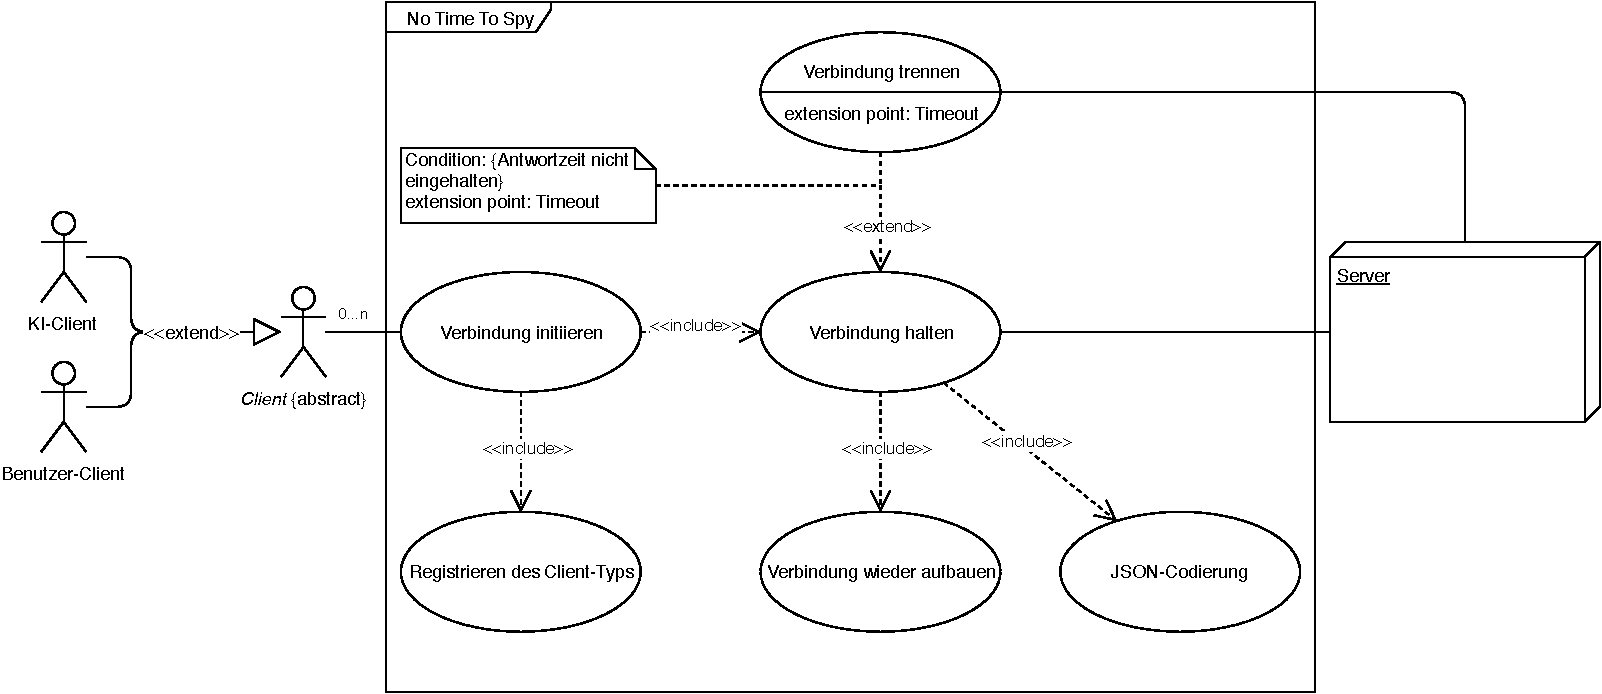
\includegraphics[width=\textwidth]{Meilenstein02/use_case_network.pdf}
  \caption{Anwendungsfälle Netzwerkverbindungsmanagement}
\end{figure}

\subsection{Verwaltung der Spielpartien bei Client und Server}
Hauptmenü anzeigen

FA-C \ref{c-menu} %FA-C 21 Hauptmenü

Anwendung beenden

FA-C \ref{c-menu} %FA-C 21 Hauptmenü

Zur Lobby-Übersicht wechseln

FA-C \ref{c-menu} %FA-C 21 Hauptmenü
FA-C \ref{c-lobby-overview} %FA-C 22 Lobby-Übersicht

Lobby-Übersicht anzeigen

FA-C \ref{c-lobby-overview} %FA-C 22 Lobby-Übersicht

Lobby-Übersicht verlassen

FA-C \ref{c-menu} %FA-C 21 Hauptmenü
FA-C \ref{c-lobby-overview} %FA-C 22 Lobby-Übersicht

Nutzernamen festlegen

FA-C \ref{c-username} %FA-C 26 Nutzername

Lobby erstellen

Konfigurationsdateien festlegen

FA-S \ref{s-partieconfig} %FA-S 1 Partie Konfiguration
FA-S \ref{s-szenarioconfig} %FA-S 2 Szenario Konfiguration
FA-S \ref{s-charakterconfig} %FA-S 3 Charakter Konfiguration

Lobby beitreten

FA-C \ref{c-join} %FA-C 23 Beitreten als Mitspieler
FA-C \ref{c-join-spectator} %FA-C 24 Beitreten als Zuschauer
FA-S \ref{s-zuschauer} %FA-S 5 Zuschauer

Lobby anzeigen

Lobby verlassen

FA-C \ref{c-lobby-overview} %FA-C 22 Lobby-Übersicht

Rolle wechseln

FA-C \ref{c-join} %FA-C 23 Beitreten als Mitspieler
FA-C \ref{c-join-spectator} %FA-C 24 Beitreten als Zuschauer
FA-S \ref{s-zuschauer} %FA-S 5 Zuschauer

Spiel starten
FA-S \ref{s-partieinit} %FA-S 8 Spiel Start und Initialisierung


\begin{figure}
  \centering
  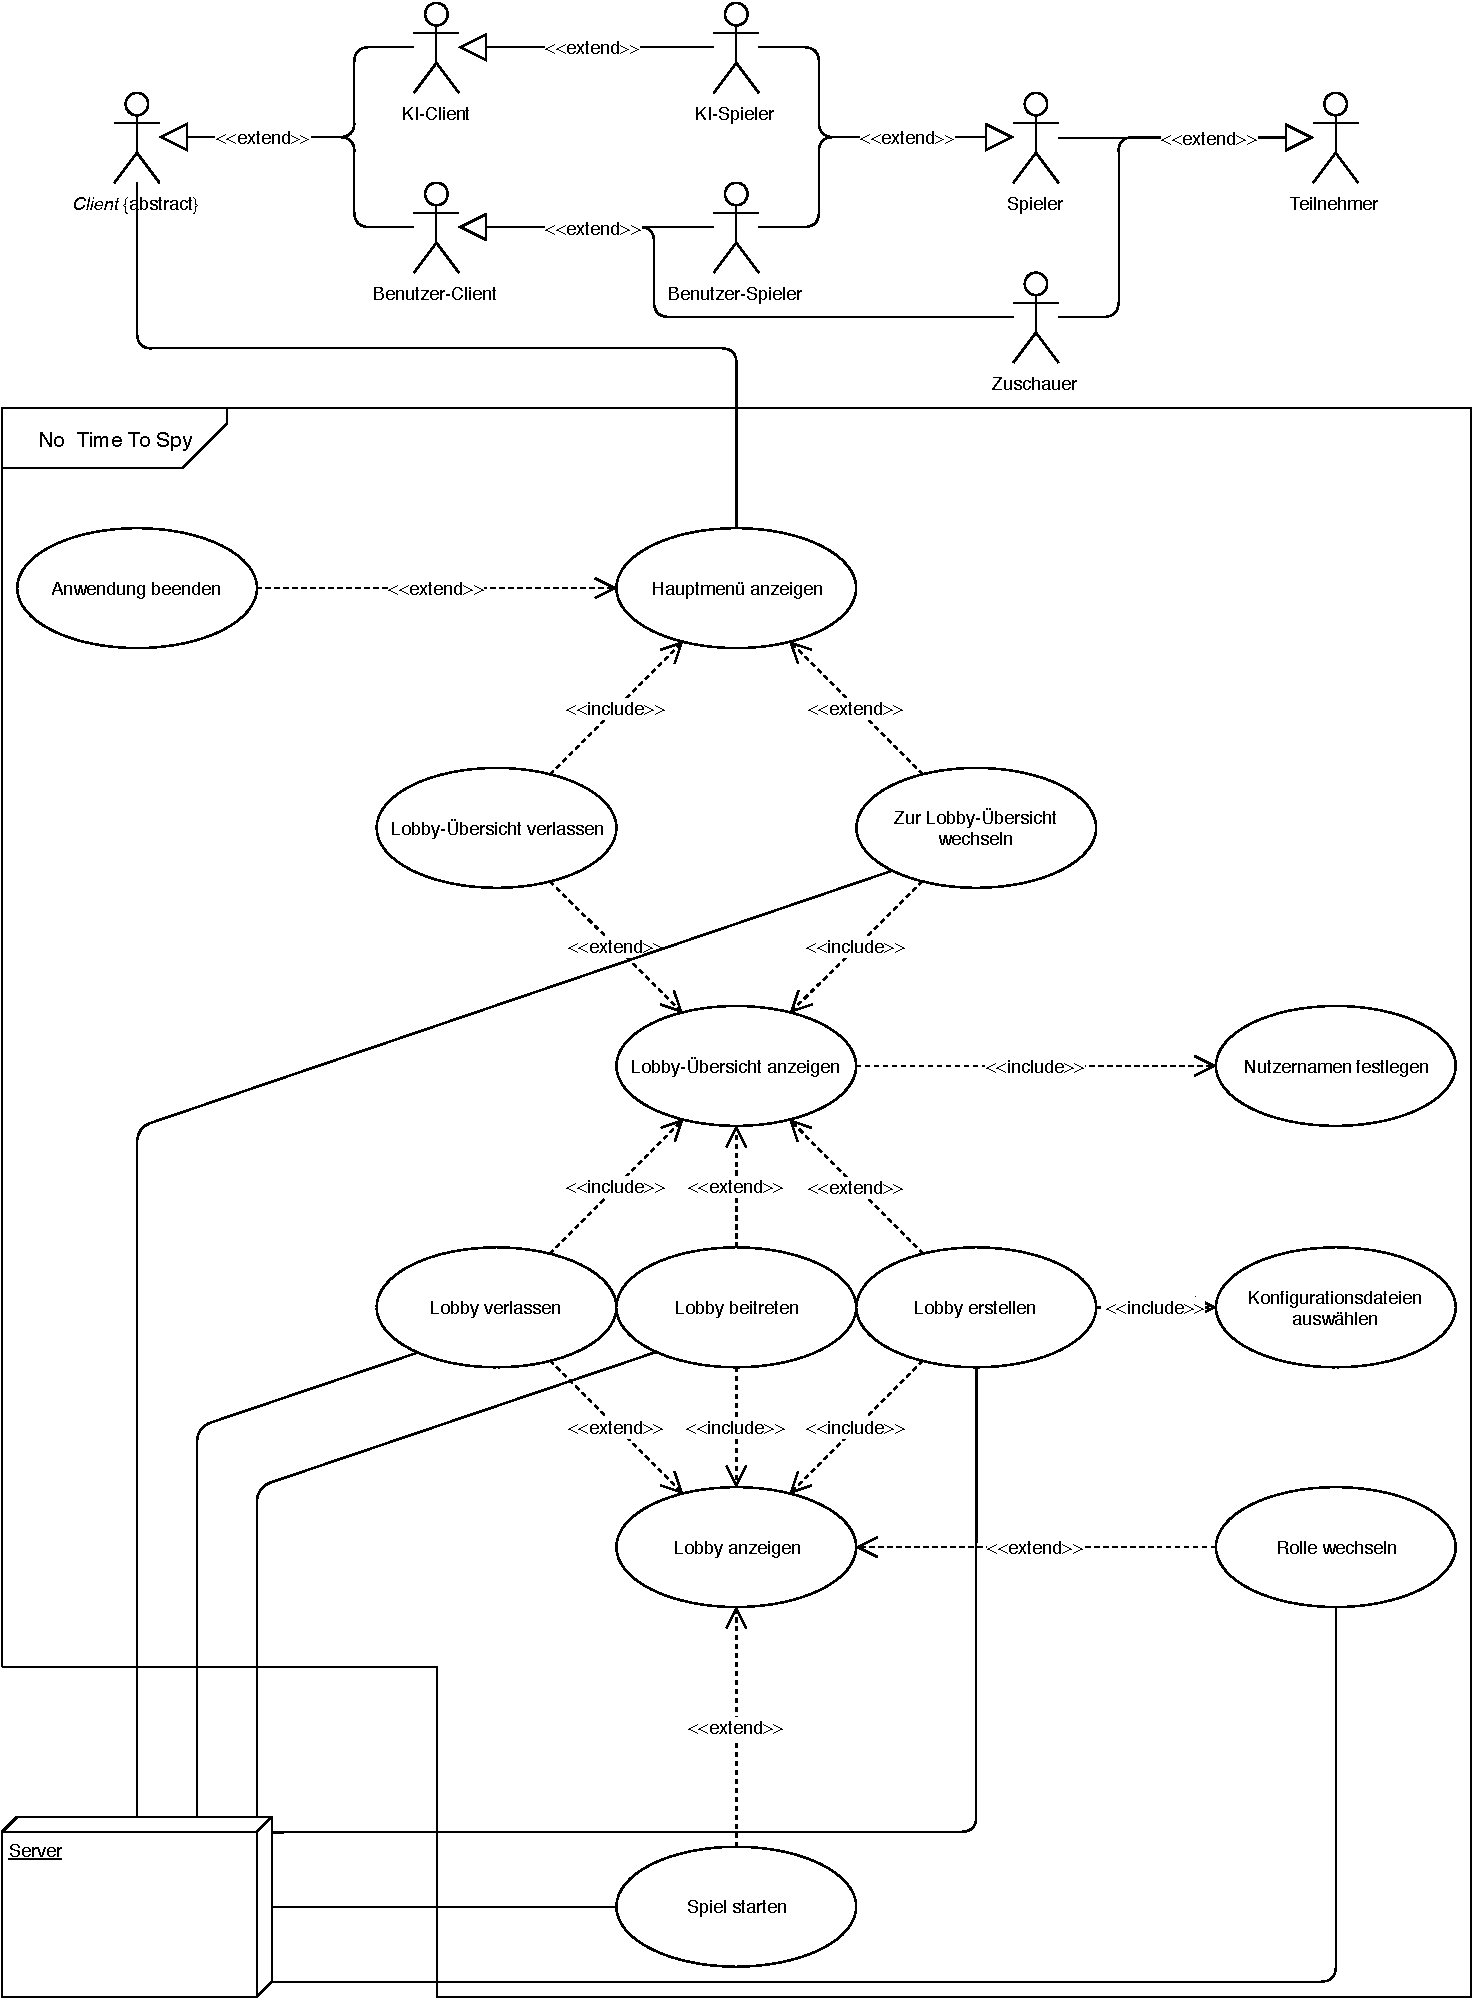
\includegraphics[width=\textwidth]{Meilenstein02/use_case_lobbymanagement.pdf}
  \caption{Anwendungsfälle Lobbymanagement}
\end{figure}

\subsection{Anwendungsfälle innerhalb einer Spielpartie}
Partie-Vorbereitung

FA-G \ref{Partie-Vorbereitung} %FA-G 126 Partie-Vorbereitung

Wahlphase

FA-G \ref{Charakter} %FA-G 64 Charakter 
FA-G \ref{Charakter Liste} %FA-G 65 Charakter Liste
FA-G \ref{Gadgets} %FA-G 94 Gadgets
FA-G \ref{Wahlphase} %FA-G 127 Wahlphase

Ausrüstungsphase
FA-G \ref{Inventar} %FA-G 74 Inventar
FA-G \ref{Gadgets} %FA-G 94 Gadgets
FA-G \ref{Ausruestungsphase} %FA-G 128 Ausrüstungsphase

Startplatzverteilung der Charaktere

FA-S \ref{s-partieinit} %FA-S 8 Spiel Start und Initialisierung
FA-G \ref{Felder} %FA-G 53 Felder
FA-G \ref{Spielbrett} %FA-G 54 Spielbrett

Zugreihenfolge festlegen

FA-S \ref{s-rundeinit} %FA-S 9 Rundenstart und Initialisierung

Spiel pausieren

FA-S \ref{s-rundeinit} %FA-S 12 Spielpause
FA-C \ref{c-pause} %FA-C 32 Wunsch auf Pausieren
FA-C \ref{c-unpause} %FA-C 33 Wunsch auf Wiederaufnahme des Spiels

Spiel fortsetzen

FA-S \ref{s-rundeinit} %FA-S 12 Spielpause
FA-C \ref{c-unpause} %FA-C 33 Wunsch auf Wiederaufnahme des Spiels

Spielbrett aktualisieren

FA-S \ref{s-state-senden} %FA-S 14 Senden des Spielzustands
FA-C \ref{c-gui} %FA-C 27 Spiel Anzeige
FA-G \ref{Spielbrett} %FA-G 54 Spielbrett

Spielbrett anzeigen

FA-C \ref{c-gui} %FA-C 27 Spiel Anzeige
FA-G \ref{Spielbrett} %FA-G 54 Spielbrett

Charakter anzeigen 

FA-C \ref{c-gui} %FA-C 27 Spiel Anzeige
FA-G \ref{Charakter} %FA-G 64 Charakter 

Feld anzeigen

FA-C \ref{c-gui} %FA-C 27 Spiel Anzeige
FA-G \ref{Felder} %FA-G 53 Felder

Spielzustand aktualisieren

FA-S \ref{s-state-senden} %FA-S 14 Senden des Spielzustands

Spielzug durchführen

FA-S \ref{s-spiel} %FA-S 10 Spiel Durchführung

Spielzug animieren

FA-C \ref{c-animation} %FA-C 31 Animation der Aktionen

Spielzug validieren

FA-S \ref{s-regeln} %FA-S 13 Erkennung von Regelverstößen

Punkt verwenden

FA-G \ref{BP und AP} %FA-G 69 Bewegungspunkte (BP) und Aktionspunkte (AP)

Bewegung durchführen

FA-G \ref{Bewegung durchfuehren} %FA-G 115 Bewegung durchführen

Drängeln

FA-G \ref{Draengeln} %FA-G 116 Drängeln

Gewinner Erkennung

FA-S \ref{s-gewinner} %FA-S 15 Gewinner Erkennung

Gewinner anzeigen

FA-C \ref{c-winnerdisplay} %FA-C 37 Gewinneranzeige

Charakter auswählen

FA-G \ref{Charakter-Position} %FA-G 67 Charakter-Position

Charakterwert anzeigen

FA-G \ref{Charakter} %FA-G 64 Charakter 

Aktion durchführen

FA-G \ref{Aktion durchfuehren} %FA-G 117 Aktion durchführen

freies Nachbarfeld finden

FA-S \ref{s-alternatives} %FA-S 11 Finden freier Felder und Alternativen

Gadget verwenden

FA-G \ref{Gadget verwenden} %FA-G 118 Gadget verwenden
FA-G \ref{Gadgets} %FA-G 94 Gadgets

Roulette spielen

FA-G \ref{Roulette spielen} %FA-G 119 Roulette spielen

Charaktereigenschaft anwenden

FA-G \ref{Eigenschaften} %FA-G 73 Eigenschaften
FA-G \ref{Bang and Burn} %FA-G 90 Bang and Burn
FA-G \ref{Observation} %FA-G 93 Observation

Spionieren

FA-G \ref{Spionieren} %FA-G 123 Spionieren

Tresor spicken

FA-G \ref{Tresor-Spicken} %FA-G 124 Tresor-Spicken

Tresorkombination erhalten

FA-G \ref{Geheimnis erhalten} %FA-G 125 Geheimnis erfahren

Cocktail-Aktion durchführen

Cocktail aufnehmen

FA-G \ref{Cocktail aufnehmen} %FA-G 120 Cocktail aufnehmen
FA-G \ref{haelt Cocktail} %FA-G 75 hält Cocktail

Jemanden mit einem Cocktail übergießen

FA-G \ref{haelt Cocktail} %FA-G 75 hält Cocktail
FA-G \ref{Cocktail-Guss} %FA-G 121 Cocktail-Guss

Cocktail schlürfen

FA-G \ref{haelt Cocktail} %FA-G 75 hält Cocktail
FA-G \ref{Cocktail schluerfen} %FA-G 122 Cocktail schlürfen



\begin{figure}
  \centering
  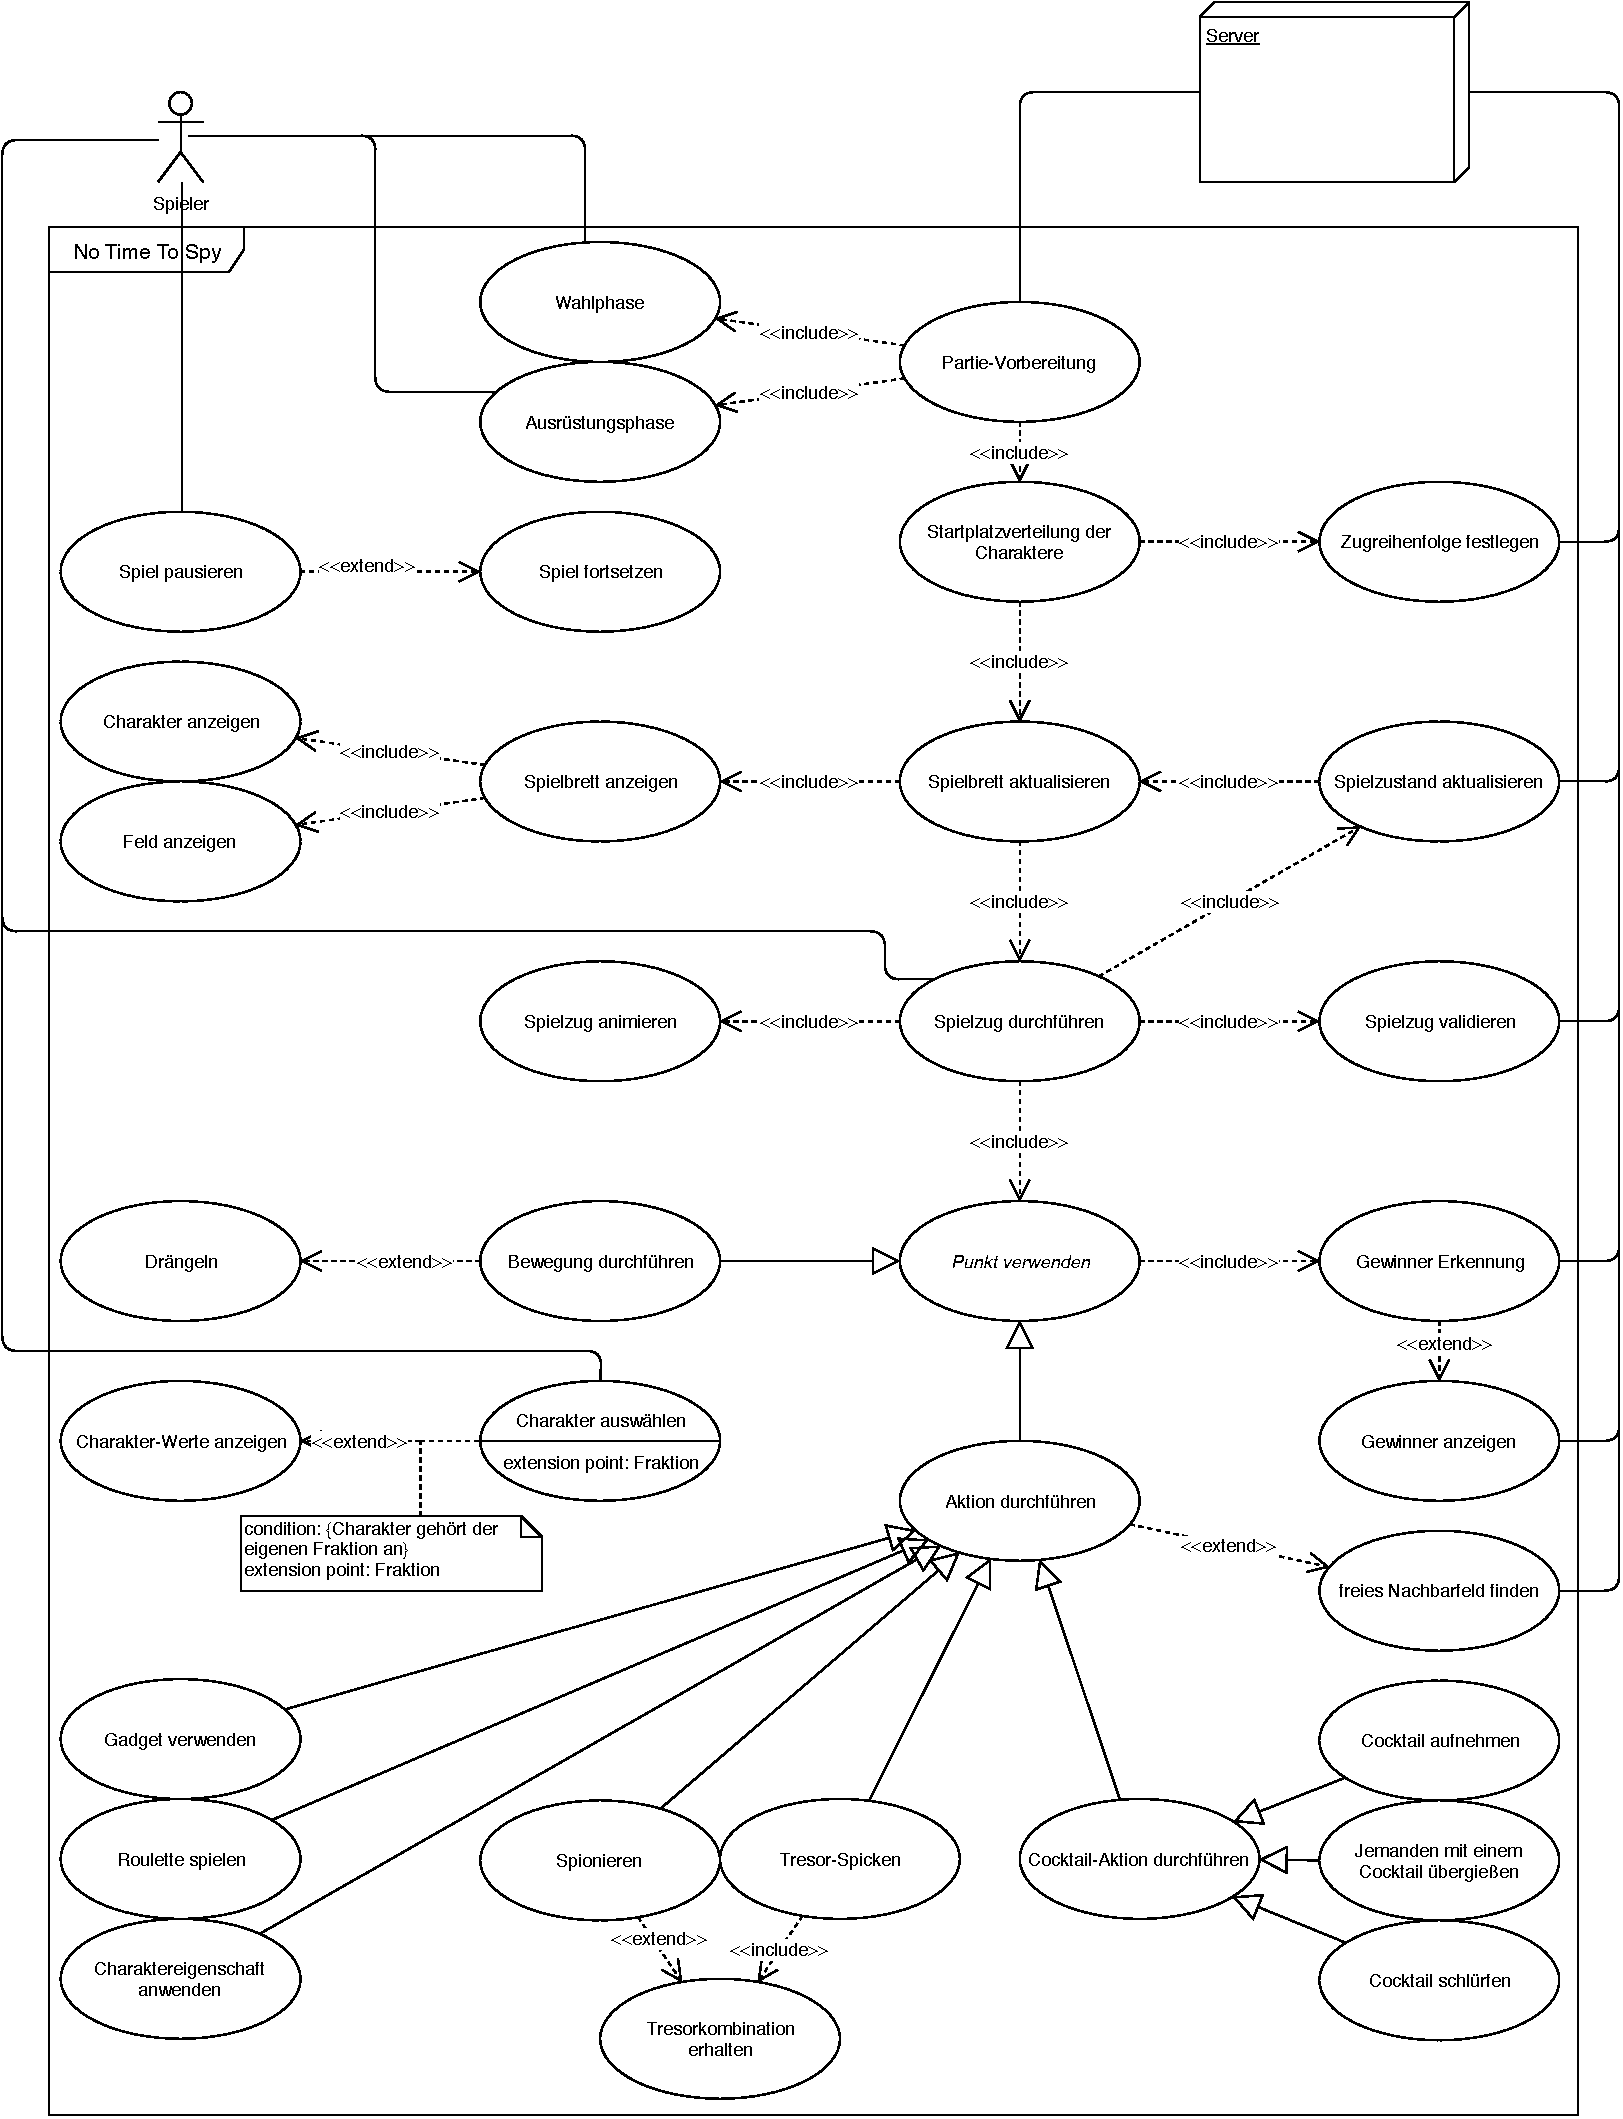
\includegraphics[width=\textwidth]{Meilenstein02/use_case_gamesession.pdf}
  \caption{Anwendungsfälle Spielpartie}
\end{figure}

\subsection{Editor}
Die drei Anwendungsfälle 'Charakterkonfiguration erstellen und editieren', Szenario-Konfiguration erstellen und editieren' und 'Partie-Konfiguration erstellen und editieren' beinhalten den Anwendungsfall 'GUI anzeigen', da es notwendig ist dem Benutzer die zu editierenden Daten graphisch anzuzeigen. Die drei erstellten Konfigurationsdateien müssen dann in das JSON-Format codiert werden. Dies wird durch den Anwendungsfall 'JSON-Datei bearbeiten' erweitert.


JSON-Datei speichern

FA-E \ref{e-json-encoding} %FA-E 47 JSON Encoding

JSON-Datei bearbeiten

FA-E \ref{e-json-decoding} %FA-E 48 JSON Decoding

GUI anzeigen

FA-E \ref{e-gui} %FA-E 49 GUI

Szenarion Konfiguration erstellen und editieren

FA-E \ref{e-szenarioedit} %FA-E 50 Szenario Editor

Partie Konfiguration erstellen und editieren

FA-E \ref{e-partieedit} %FA-E 51 Partie Editor

Charakter Konfiguration erstellen und editieren

FA-E \ref{e-charedit} %FA-E 52 Charakter Editor

\begin{figure}
  \centering
  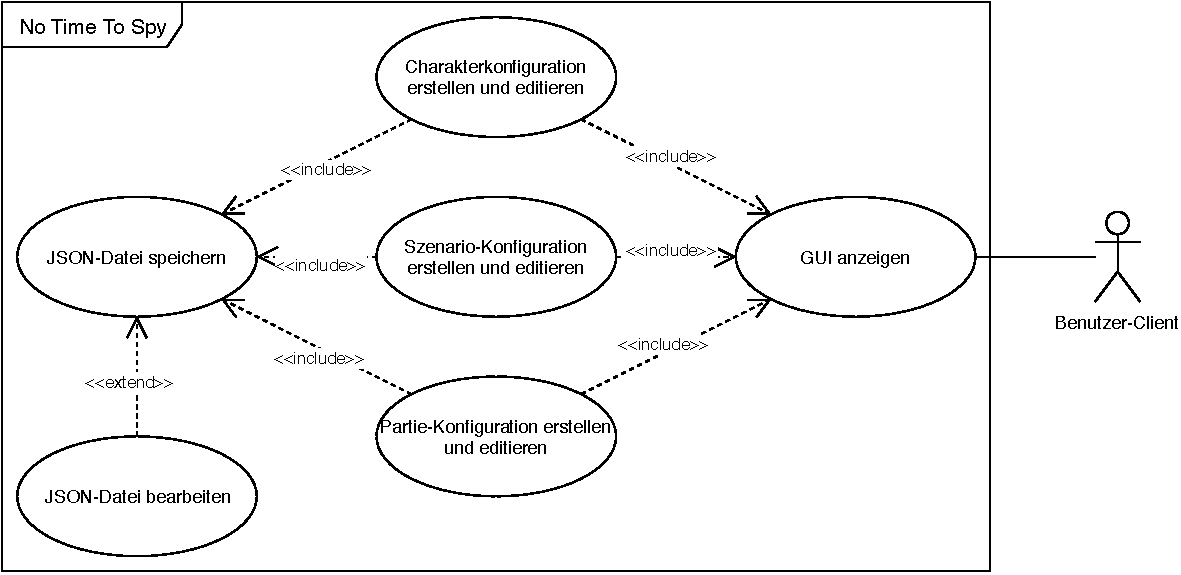
\includegraphics[width=\textwidth]{Meilenstein02/use_case_editor.pdf}
  \caption{Anwendungsfälle Editor}
\end{figure}

\section{Abläufe im System}
\subsection{Verbindungsaufbau zum Server}
\subsection{Verbindung mit dem Server}

\begin{tikzpicture} 
    \begin{umlseqdiag} 
        \umlactor[class=Spieler]{P1}
        \umlobject[no ddots]{Server}
        \umlactor[class=Spieler]{P2}
        
        \begin{umlcall}[op={register}, return={Success}]{P1}{Server}
            \begin{umlcall}[op={name(String)}]{P1}{Server} 
            \end{umlcall}
            
            \begin{umlfragment}[type=alt, label=Mensch, inner xsep=7] 
                \begin{umlcall}[op={type("Mensch")}]{P1}{Server} 
                \end{umlcall}

                \umlfpart[KI]

                \begin{umlcall}[op={type("KI")}]{P1}{Server}
                \end{umlcall}
            \end{umlfragment}

        \end{umlcall}

        \begin{umlcall}[dt=35, op={register}, return={Success}]{P2}{Server}
            \begin{umlcall}[op={name(String)}]{P2}{Server} 
            \end{umlcall}
            
            \begin{umlfragment}[type=alt, label=Mensch, inner xsep=7] 
                \begin{umlcall}[op={type("Mensch")}]{P2}{Server} 
                \end{umlcall}

                \umlfpart[KI]

                \begin{umlcall}[op={type("KI")}]{P2}{Server}
                \end{umlcall}
            \end{umlfragment}

        \end{umlcall}

        \begin{umlcall}[op=ready]{Server}{P1}
            \begin{umlcall}[op=ready, dt=-1]{Server}{P2}
            \end{umlcall}
        \end{umlcall}

        \begin{umlfragment}[type=alt, label=P1, inner xsep=7] 
            \begin{umlcall}[op=start, dt=10]{P1}{Server} 
            \end{umlcall}

            \umlfpart[P2]

            \begin{umlcall}[op=start, dt=20]{P2}{Server}
            \end{umlcall}
        \end{umlfragment}

    \end{umlseqdiag} 
\end{tikzpicture}


\subsection{Beitreten einer Lobby}
\begin{tikzpicture}
\begin{umlseqdiag} 
	\umlactor[class=Mensch-Spieler]{P1}
	\umlobject[no ddots]{Server}
	\umlactor[class=Spieler]{P2}

	
	\begin{umlcall}[op=newLobby(String), dt=5]{P1}{Server}
		\begin{umlcall}[type=return, op=lobbyCreated]{Server}{P1}
		\end{umlcall}
		
		\begin{umlcall}[op=joinLobby(String)]{P1}{Server}
			\begin{umlcall}[type=return, op=lobbyInfo]{Server}{P1}
			\end{umlcall}
		\end{umlcall}
	
	
		\begin{umlfragment}[type=alt, label=Mensch, inner xsep=7]
			\begin{umlcall}[op=joinLobby(String), dt=25]{P2}{Server}
				\begin{umlcall}[type=return, op=lobbyInfo]{Server}{P2}
				\end{umlcall}
			\end{umlcall}
			
			\umlfpart[KI]
			
			\begin{umlcall}[op=lobbyInfo]{Server}{P2}
			\end{umlcall}
		\end{umlfragment}
		
	\end{umlcall}
    
\end{umlseqdiag}
\end{tikzpicture}

\subsection{Durchführen einer Aktion}
In jeder Runde legt der Server eine Zugreihenfolge für die Charaktere fest und berechnet deren Bewegungs- und Aktionspunkte. Hier ist gerade ein Charakter aus der Fraktion von P1 am Zug. Ein Zug kann entweder eine Bewegung oder eine Aktion sein. Die dargestellte Sequenz wiederholt sich solange bis der Charakter von P1 keine BP und AP mehr hat oder P1 den Zug beendet. Anschließend ist der nächste Charakter an der Reihe.\\

\begin{tikzpicture}
    \begin{umlseqdiag}
        \umlactor[class=Client]{P1}
        \umlobject[no ddots]{Server}
        \umlactor[class=Client]{P2}

        \begin{umlcall}[op=zug]{P1}{Server}

            \begin{umlcallself}[op=validate]{Server}
            \end{umlcallself}

            \begin{umlfragment}[type=alt, label=fail, inner xsep=8]

                \begin{umlcall}[type=return, op=fail]{Server}{P1}
                \end{umlcall}

                \umlfpart[success]

                \begin{umlcall}[op=zug(result)]{Server}{P2}
                \end{umlcall}

                \begin{umlcall}[type=return, op=zug(result)]{Server}{P1}
                \end{umlcall}

            \end{umlfragment}

        \end{umlcall}

    \end{umlseqdiag}
\end{tikzpicture}


\subsection{Aktualisieren des Spielfelds}
\begin{tikzpicture}
    \begin{umlseqdiag}
        \umlactor[class=Zuschauer]{W}
        \umlobject[no ddots]{Server}
        \umlactor[class=Spieler]{P}

        \begin{umlcall}[op=action(result)]{Server}{P}
	        \begin{umlcall}[op=action(result)]{Server}{W}
	        \end{umlcall}

            \begin{umlcallself}[op=updateView]{W}
            \end{umlcallself}
            
			\begin{umlfragment}[type=alt, label=Mensch, inner xsep=5]

				\begin{umlfragment}[type=alt, label=wasTurn, inner xsep=9]
					\begin{umlcallself}[op=validateView, dt=15]{P}
					\end{umlcallself}
					
					\umlfpart[wasNotTurn]
					
					\begin{umlcallself}[op=updateView]{P}
					\end{umlcallself}
				\end{umlfragment}
			
				\umlfpart[KI]
				
				\begin{umlcallself}[op=updateModel]{P}
				\end{umlcallself}
			\end{umlfragment}
            

        \end{umlcall}

    \end{umlseqdiag}
\end{tikzpicture}


\subsection{Spielende und Abbau der Verbindung zum Server}
\begin{tikzpicture} 
    \begin{umlseqdiag} 
        \umlactor[class=Spieler]{P1}
        \umlobject[no ddots]{Server}
        \umlactor[class=Spieler]{P2}
        
        \begin{umlcall}[op={action(result)}]{Server}{P2}
        \begin{umlcall}[type=return, op={action(result)}]{Server}{P1}
            
            \begin{umlfragment}[type=alt, label=Winner, inner xsep=8]
             
             	\begin{umlfragment}[type=alt, label=Mensch, inner xsep=4]
	             	\begin{umlcallself}[op=displayWinner]{P1}
	             	\end{umlcallself}
	             	
	             	\umlfpart[KI]
	             	
	             	\begin{umlcallself}[op=infoWinner]{P1}
	             	\end{umlcallself}
             	\end{umlfragment}
             	
             	\begin{umlfragment}[type=alt, label=Mensch, inner xsep=7]
	             	\begin{umlcallself}[op=displayWinner]{P2}
	             	\end{umlcallself}
	             	
	             	\umlfpart[KI]
	             	
	             	\begin{umlcallself}[op=infoWinner]{P2}
	             	\end{umlcallself}
             	\end{umlfragment}
             	
             	\begin{umlcall}[op={deregister}, dt=7]{P1}{Server}
             	\begin{umlcall}[op={deregister}, dt=10]{P2}{Server}
             	
				\end{umlcall}
				\end{umlcall}

            \end{umlfragment}
            
            
		\end{umlcall}
        \end{umlcall}

    \end{umlseqdiag} 
\end{tikzpicture}

\clearpage

\subsection{Zustände im Spiel}
Hier kommt das Spiel Zustandsdiagramm hin

\clearpage
\subsubsection{Wahl- und Ausrüstungsphase}
In diesem Diagramm wird die Wahl- und Ausrüstungsphase durch ein Sequenzdiagramm beschrieben.

\begin{tikzpicture}
	\begin{umlseqdiag}
		\umlactor[class=Spieler]{P1}
		\umlactor[no ddots]{Server}
		\umlactor[class=Spieler]{P2}

		\begin{umlfragment}[type=Wahlphase,inner xsep=7]
			\begin{umlcall}[op={3 Char./ 3 Gadgets},dt=10,return={Gewähltes Gadget/Char.},padding=5]{Server}{P1}
			\end{umlcall}
			\begin{umlcall}[op={3 Char./ 3 Gadgets},dt=-6,return={Gewähltes Gadget/Char.},padding=5]{Server}{P2}
			\end{umlcall}
		\end{umlfragment}

		

		\begin{umlfragment}[type=Ausrüstungsphase,inner xsep=7]
			\begin{umlcall}[op={Gadget auf Char.},dt=10,return={Bestätigung},padding=5]{P1}{Server}
			\end{umlcall}
			\begin{umlcall}[op={Gadget auf Char.},dt=10,return={Bestätigung},padding=5]{P2}{Server}
			\end{umlcall}
		\end{umlfragment}
	\end{umlseqdiag}
\end{tikzpicture}

In der Wahlphase bietet der Server jedem Spieler drei Charaktere und drei Gadgets zur Auswahl an. 
Es wird dabei durch den Server sichergestellt, dass die Spieler nicht das gleiche Gadget oder den gleichen Charakter wählen können.\\
Eine vom Spieler zusammengestellte Fraktion besteht aus zwei bis vier Charakteren.
Insgesamt wird die im Diagramm beschriebene Wahlphase acht mal wiederholt.\\

In der Ausrüstungsphase muss jeder Spieler seine gewählten Gadgets einem seiner Agenten zuordnen. Die im Diagramm beschriebene Ausrüstungsphase wird solange wiederholt, bis alle Gadgets einem Charakter zugeordnet sind.

\clearpage

\clearpage
\subsection{Zustände des Clients}
%Found at: %https://tex.stackexchange.com/questions/420217/change-style-of-basic-states-in-tikz-uml-package
\tikzset{singlestate/.style={draw,fill=yellow!20, rounded corners, align=center}}

\begin{tikzpicture}
	\umlstateinitial[name=initial, x=0, y=0]
	\begin{umlstate}[x=7, y=-2, name=menu]{Hauptmenü}
		\umlstatetext{}
		\umlbasicstate[x=0, y=0, name=menuDisconnected, do={bekannte Server\\ anpingen}, align=center]{Hauptmenü (disconnected)}
		\umlbasicstate[x=0, y=-4, name=menuConnected, do={Lobbies abfragen}]{Hauptmenü (connected)}
	\end{umlstate}
	
	\node[singlestate] at (0, -2.7) (help){Hilfe};
	\node[singlestate] at(16, -4.85) (settings){Einstellungen};
	\umlstatefinal[x=16, y=-0, name=final]
	\node[singlestate] at (7, -8) (lobbyView){Lobbyübersicht};
	
	\begin{umlstate}[x=7, y=-13, name=lobby]{Lobby}
		\umlstatetext{}
		\umlbasicstate[x=0, y=0, name=spieler, do={}, align=center]{in Lobby (Rolle: Spieler)}
		\umlbasicstate[x=0, y=-4, name=zuschauer, do={}]{in Lobby (Rolle: Zuschauer)}
	\end{umlstate}
	
	\node[singlestate] at (7, -20) (inGame){im Spiel};
	\node[singlestate] at (7, -22) (gameEnded){Spiel beendet};
	
	\umlVHtrans{initial}{menuDisconnected}
	
	\umltrans[align=center, arg={verbinde/}, pos=0.5, align=right, anchor1=-120, anchor2=125]{menuDisconnected}{menuConnected}
	\umltrans[arg={trennen/}, pos=0.5, align=left, anchor1=55, anchor2=-60]{menuConnected}{menuDisconnected}
	
	\umlHVtrans[arg={Hilfe aufrufen/}, pos=0.5, align=right, anchor1=160]{menu}{help}
	\umlVHtrans[arg={Hilfe schließen/}, pos=0.5, anchor2=200]{help}{menu}
	
	\umlHVtrans[arg={Einstellungen aufrufen/}, pos=0.8, align=right, anchor1=-30]{menu}{settings}
	\umlVHtrans[arg={Einstellungen schließen/}, pos=1.2, anchor1=-90, anchor2=-48, align=right]{settings}{menu}
	
	\umlHVtrans[arg={Client schließen/}, pos=0.7, align=right, anchor1=30]{menu}{final}
	
	\umltrans[arg={Lobbyübersicht aufrufen/}, pos=0.7, align=right, anchor1=-127, anchor2=158]{menuConnected}{lobbyView}
	\umltrans[arg={Zurück zum Menü/}, pos=0.3, align=left, anchor1=23, anchor2=-56]{lobbyView}{menuConnected}
	
	\umltrans[arg={verlasse Lobby/}, pos=0.4, align=left, anchor1=90, anchor2=-90]{lobby}{lobbyView}
	
	\umlHVHtrans[arg={betrete Lobby[Spielerslots belegt]/}, pos=1.5, align=left, anchor1=0, anchor2=0, arm1=2cm]{lobbyView}{zuschauer}
	\umlHVHtrans[arg={betrete Lobby[Spielerslot frei]/}, pos=1.5, align=right, anchor1=180, anchor2=180, arm1=-2cm]{lobbyView}{spieler}
	
	\umltrans[arg={Rollenwechsel/}, pos=0.5, align=right, anchor1=-110, anchor2=110]{spieler}{zuschauer}
	\umltrans[arg={Rollenwechsel/}, pos=0.5, align=left, anchor1=70, anchor2=-70]{zuschauer}{spieler}
	
	\umlHVHtrans[arg={Zurück zum Menü/}, pos=0.2, align=left, arm1=8.5cm, anchor2=-15]{gameEnded}{menuConnected}
	
	\umltrans[arg={Spielende erreicht/}, pos=0.6, align=left]{inGame}{gameEnded}
	
	\umltrans[arg={Spiel starten[alle Spieler bereit]/}, pos=0.6, align=left]{lobby}{inGame}
%
\end{tikzpicture}

\subsection{Zustände des KI-Clients}
Das untenstehende Zustandsdiagramm gibt einen kleinen Überblick über die grobe Funktionsweise des KI-Clients. 

\begin{tikzpicture} 
    \umlstateinitial[y=4, name=initial]
    \begin{umlstate}[name=running]{running}
        \begin{umlstate}[name=waiting, y=0]{Warte}
        \end{umlstate}

        \begin{umlstate}[name=analyzing, y=-4]{Analysiere Spielzustand}
        \end{umlstate}

        \begin{umlstate}[name=planning, y=-8]{Plane nächste Aktion}
        \end{umlstate}

        \umlHVHtrans[arm1=5, arg={Aktion Senden}, pos=0.5]{planning}{waiting}
        \umltrans[arg={Aktion Empfangen}, pos=0.5]{waiting}{analyzing}
        \umltrans{analyzing}{planning}

    \end{umlstate}

    \umltrans[arg={verbinde/}, pos=0.3]{initial}{waiting}
    \umlstatefinal[name=final, x=-6, y=-1]
    \umlHVtrans[arg={Spielende erreicht/}, pos=0.6]{waiting}{final}
\end{tikzpicture}


\subsection{Zustände des Servers}
Im Folgenden wird ein Ausschnitt der Zustände des Servers betrachtet. Um das Zustandsdiagramm übersichtlich zu halten werden lediglich zwei Spieler und keine Zuschauer modelliert. Außerdem wird davon ausgegangen, dass die beiden Clients sich entsprechend Abschnitt \ref{connect} bereits beim Server registriert haben.  

\tikzset{singlestate/.style={draw,fill=yellow!20, rounded corners, align=center}}

\begin{tikzpicture} 
    \umlstateinitial[x=5, y=2, name=initial]
    \umlbasicstate[x=5, y=-1, name=initialize, do={erstelle Standard-Lobby}, align=center]{Initialisierung}
    \begin{umlstate}[x=0, y=-5, name=running]{running}
	    \begin{umlstate}[y=0, name=lobby]{Lobby}
	    	\umlstatetext{}
	    	\umlbasicstate[x=0,  y=-1, name=emptyLobby, do={}, align=center]{Leere Lobby}
	    	\umlbasicstate[x=10, y=-1, name=waitSecond, do={}, align=center]{Warte auf zweiten Spieler}
	    	\umlbasicstate[x=5, y=-5, name=startable, do={erlaube Spielstart}, align=center]{Spiel startbereit}
	    \end{umlstate}
	    \umlbasicstate[x=1,  y=-8, name=game, do={gampeplay}, align=center]{Spiel}
	    \umlbasicstate[x=11, y=-7.8, name=paused, do={}, align=center]{Spiel pausiert}
	    \umlbasicstate[x=10, y=-10, name=disconnect, do={}, align=center]{Warte auf Reconnect}
    \end{umlstate}
    
    \umlbasicstate[x=3, y=-19, name=deinitialize, do={beende laufende Spiele}, align=center]{Deinitialisierung}
    \umlstatefinal[x=10, y=-18.5, name=final]

    \umltrans{initial}{initialize}
    \umltrans[anchor1=-90, anchor2=93]{initialize}{running}
    \umltrans[arg={Spieler 1 tritt bei/}, pos=0.5, anchor1=15.5, anchor2=170]{emptyLobby}{waitSecond}
    \umltrans[arg={Spieler 1 verlässt Lobby/}, pos=0.5, anchor1=-170, anchor2=-15.5]{waitSecond}{emptyLobby}
    \umlVHtrans[arg={Spieler 2 tritt bei/}, pos=0.5, anchor1=-140, anchor2=20, align=right]{waitSecond}{startable}
    \umlHVtrans[arg={Spieler 2 verlässt Lobby/}, pos=0.5, anchor1=-20, anchor2=-40, name=exit2]{startable}{waitSecond}
    \umlHVtrans[arg={Spielstart/Spieler*.gameStarted}, pos=0.01, anchor1=+160, anchor2=90, align=right]{startable}{game}
    \umltrans[arg={Spiel pausieren[Mensch-Spieler]/Spieler*.pause}, pos=0.5, anchor1=15.5, anchor2=157]{game}{paused}
    \umltrans[arg={Spiel fortsetzen/Spieler*.continue}, pos=0.5, anchor1=-170, anchor2=-15.5]{paused}{game}
    
    \umlVHtrans[arg={Spieler Verbindungsabbruch/Spieler*.notify}, pos=0.9, anchor1=-40, anchor2=160, align=left]{game}{disconnect}
    \umlHVtrans[arg={Spieler Reconnect/Spieler*.gameContinues}, pos=0.9, anchor1=-160, anchor2=-80, align=left]{disconnect}{game}
    
    \umltrans[arg={Shutdown Server/}, pos=0.5]{running}{deinitialize}
    \umltrans{deinitialize}{final}
    
    \umlHVHtrans[arg={Spielende/Spieler*.redirectLobby}, anchor1=-180, anchor2=160, arm1=-3cm]{game}{lobby}
    
    \umlnote[x=10,y=0]{waitSecond}{Spieler 1 könnte die Lobby ebenfalls verlassen (gewollt oder wegen eines Verbindungsabbruchs), in diesem Fall wird der bisherige Spieler 2 nun zu Spieler 1.}
\end{tikzpicture}

\clearpage

\section{Schnittstellenarten und Dialogstruktur}
\subsection{Schnittstellenbeschreibung des Clients}
Für den Client wird eine graphische Benutzerschnittstelle gewählt.
Eine solche bietet dem Benutzer eine einfache Bedienung und ermöglicht es komplexe Zusammenhänge einfach für den Spieler darzustellen.
Des weiteren bietet eine graphische Benutzerschnittstelle mehr Möglichkeiten, wie der Spieler mit dem Spiel interagieren kann als eine Kommanozeilenanwendung.\\

Im folgenden werden die einzelnen Dialoge und Popups aufgelistet und welche Anwendungsfälle diese jeweils abdecken

\begin{itemize}
	\item Dialog Hauptmenü: Hauptmenü anzeigen, Anwendung beenden, zur Lobbyübersicht wechseln, Einstellungen, Hilfe anzeigen
	\item Dialog Einstellungen: Vornehmen von Einstellungen
	\item Popup Hilfe: Anzeigen von Hilfsfunktionen
	\item Popup Fehler bei der Verbindung zum Server: Übergang zur Lobbyübersicht, Fehlerfall
	\item Dialog Lobbyübersicht: Lobbyübersicht anzeigen, Lobbyübersicht verlassen, Lobby erstellen, Lobby beitreten, Nutzernamen festlegen
	\item Popup Nutzernamen ändern: Nutzernamen festlegen
	\item Popup Lobbyname eingeben und Konfig. erstellen: Konfigurationsdaten festlegen
	\item Dialog Editor: erstellen von Konfigurationsdaten
	\item Dialog Lobby: Lobby anzeigen
	\item Popup Rolle ändern: Rolle wechseln
	\item Popup Konfiguration anzeigen: anzeigen der Konfiguration
	\item Dialog Wahlphase: Wahlphase anzeigen, Character/Gadget wählen
	\item Dialog Ausrüstungsphase: Ausrüstungsphase anzeigen, Gadget zuweisen
	\item Dialog Spielbildschirm: Spielbildschirm anzeigen, Spielstand darstellen, Spielaktion durchführen, Spiel verlassen
	\item Popup Optionen: Einstellungen, Spiel pausieren
	\item Popup Einstellungen: Einstellungen vornehmen
	\item Popup Pausieren: Spiel pausieren und entpausieren
	\item Dialog Gewinnerbildschirm: Gewinnerbildschirm anzeigen, Gewinner zeigen, Statistiken anzeigen
\end{itemize}

Im Spielbildschirm wurden alle möglichen Aktionen die ein Spieler durchführen kann aus Übersichtlichkeitsgründen zu \textit{Spielaktion durchführen} zusammengefasst. Dazu gehören Charakter anzeigen, Feld anzeigen, Charakter bewegen, Gadget verwenden, etc.
\begin{figure}
  \centering
  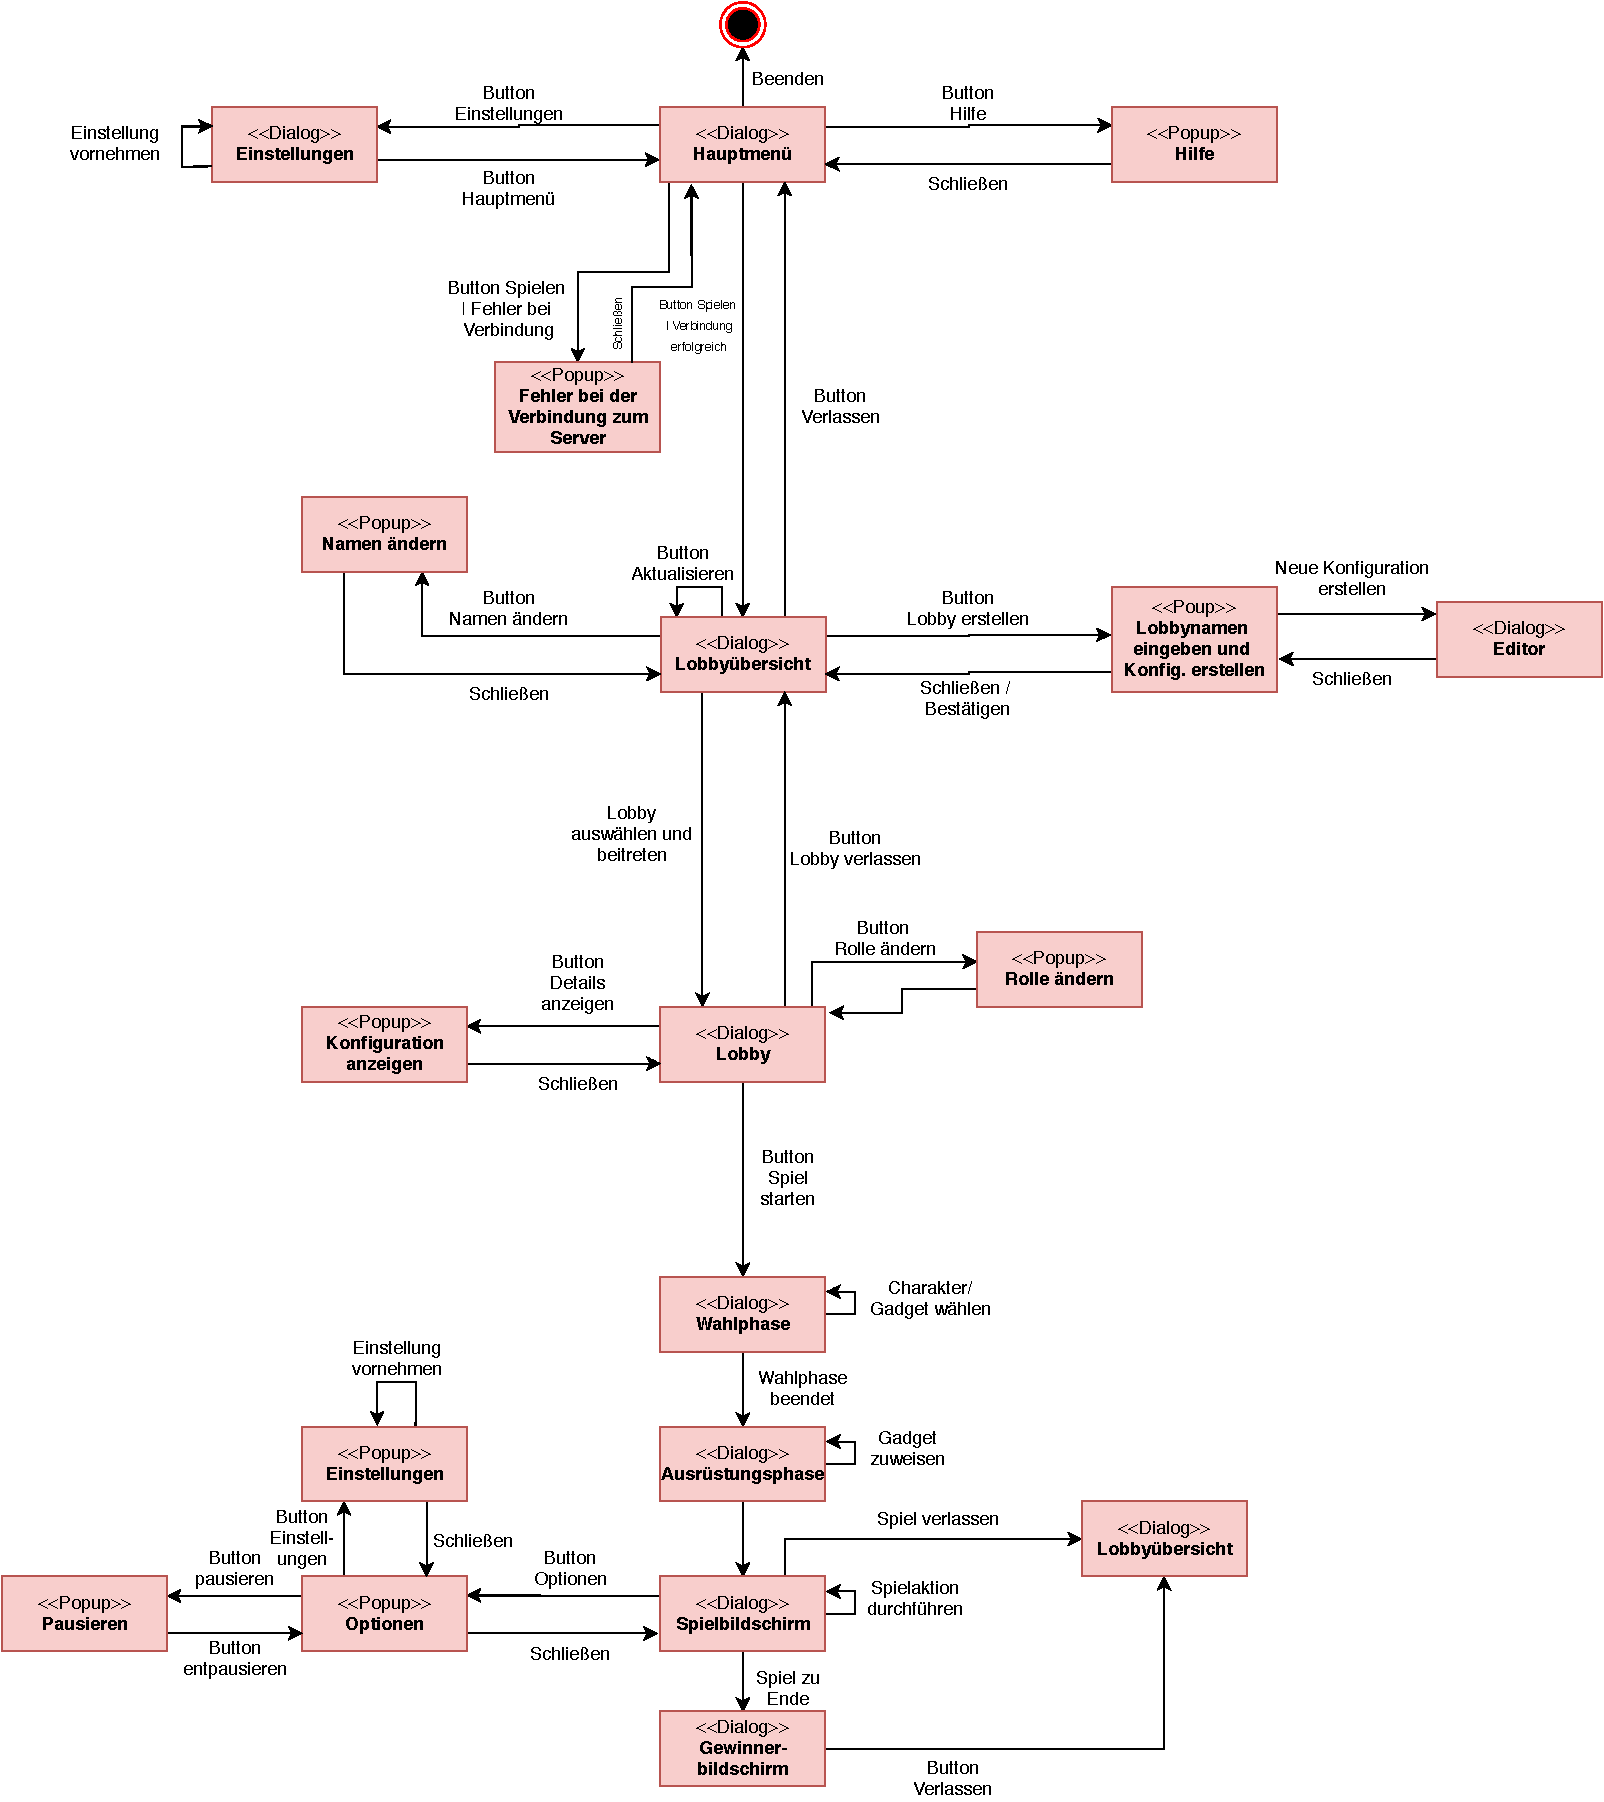
\includegraphics[width=\textwidth]{Meilenstein03/client_dialog.pdf}
  \caption{Dialog Diagram für den Client}
\end{figure}

\clearpage

\subsection{Schnittstellenbeschreibung des Servers}
Der Server wird über die Kommandozeile in einem Docker-Container gestartet (QA2).\\
Mit den Clients (jeglicher Art) kommuniziert er über eine Websocket-Verbindung (FA-S \ref{s-websockets}), über welche Nachrichten im JSON-Format ausgetauscht werden (FA-S \ref{s-json-encoding}, FA-S \ref{s-json-decoding}).
\clearpage

\subsection{Schnittstellenbeschreibung des Editors}
Erstellt ein Benutzer-Client über die Lobbyübersicht eine neue Lobby, so muss er die Konfiguration des Editors über eine graphische Oberfläche durchführen (FA-E \ref{e-gui}, FA-E \ref{e-szenarioedit}, FA-E \ref{e-partieedit}, FA-E \ref{e-charedit}).

\begin{figure}[h]
	\centering
	\tikzstyle{block} = [draw, rectangle, 
	minimum height=3em, minimum width=6em, very thick, align = center]
	\begin{tikzpicture}[auto, node distance=2cm,>=latex']
	
	\node[block] (Editor) at (0, 7) {<<Dialog>>\\ \textbf{Editor}};
	
	\node[block, above left = 1.0cm and 1.0cm of Editor] (Help) {<<Popup>>\\ \textbf{Help}\\ (QA10)};
	
	\node[block, below left = 3.0cm and 3.0cm of Editor] (Szenario) {<<Dialog>>\\ \textbf{Szenario-Editor}};
	
	\node[block, below = 3.0cm of Editor] (Partie) {<<Dialog>>\\ \textbf{Partie-Editor}};
	
	\node[block, below right = 3.0cm and 3.0cm of Editor] (Charakter) {<<Dialog>>\\ \textbf{Charakter-Editor}};
	
	\node[block, above right = 1.0cm and 1.5cm of Editor] (Lobby) {<<Dialog>>\\ \textbf{Create Lobby}};
	
	
	\draw[thick, ->, shorten >=1mm,shorten <=1mm] (Editor.west) -| (Help.south) node [near start, xshift=3mm] {\small Help};
	\draw[thick, ->, shorten >=1mm,shorten <=1mm] (Help.east) -| ([xshift= -0.5cm]Editor.north) node [near start, xshift=3mm] {\small Close};
	
	\draw[thick, ->, shorten >=1mm,shorten <=1mm] (Editor.east) -| (Lobby.south) node [near start, xshift=1.5mm] {\small Save $\vert\vert$ Back};
	\draw[thick, ->, shorten >=1mm,shorten <=1mm] (Lobby.west) -| ([xshift= 0.5cm]Editor.north) node [near start, xshift=3mm] {\small Configure};
	
	\draw[thick, ->, shorten >=1mm,shorten <=1mm] ([xshift = -0.5cm]Editor.south) -- (Szenario.north) node [near start, xshift=-30mm, yshift = -5mm] {\small Szenario};
	\draw[thick, ->, shorten >=1mm,shorten <=1mm] (Szenario.east) -- (Partie.west) node [near start, xshift=3mm] {\small Partie};
	\draw[thick, ->, shorten >=1mm,shorten <=1mm] (Partie.east) -- (Charakter.west) node [near start, xshift=3mm] {\small Charakter};
	\draw[thick, ->, shorten >=1mm,shorten <=1mm] (Charakter.north) -- ([xshift = 0.5cm]Editor.south) node [near start, xshift=4mm, yshift = 10mm] {\small Editor};
	
	
	
	\end{tikzpicture}
	\caption{graphische Schnittstelle des Editors}
\end{figure}

Um die Konfiguration, die im Editor vorgenommen wurde, über die Websocket-Schnittstelle des Mensch-Clients mit dem Server zu kommunizieren, verfügt der Editor über eine JSON-Schnittstelle (FA-E \ref{e-json-encoding}, FA-E \ref{e-json-decoding}).
\clearpage

\subsection{Schnittstellenbeschreibung des KI-Clients}
Die KI kommuniziert mit dem Server über eine Websocket Verbindung (FA-KI \ref{ki-session}, FA-KI \ref{ki-register}).\\
Mit dem Mensch-Client interagiert die KI über eine graphische Oberfläche, die der Mensch-Client implementiert. Dabei hat der Mensch-Client in der Lobby die Möglichkeit eine KI als gegnerischen Spieler hinzuzufügen (FA-KI \ref{ki-config}, FA-KI \ref{ki-intelligenz}).

\begin{figure}[h]
	\centering
	\tikzstyle{block} = [draw, rectangle, 
	minimum height=3em, minimum width=6em, very thick, align = center]
	\begin{tikzpicture}[auto, node distance=2cm,>=latex']
	
	\node[block] (KI) at (0, 7) {<<Dialog>>\\ \textbf{KI-Configuration}};
	
	\node[block, below left = 1.0cm and 1.0cm of KI] (Help) {<<Popup>>\\ \textbf{Help}\\ (QA10)};
	
	\node[block, above right = 1.0cm and 1.5cm of KI] (Lobby) {<<Dialog>>\\ \textbf{Lobby}};
	
	
	\draw[thick, ->, shorten >=1mm,shorten <=1mm] (KI.west) -| (Help.north) node [near start, xshift=3mm] {\small Help};
	\draw[thick, ->, shorten >=1mm,shorten <=1mm] (Help.east) -| (KI.south) node [near start, xshift=3mm] {\small Close};
	
	\draw[thick, ->, shorten >=1mm,shorten <=1mm] (KI.east) -| (Lobby.south) node [near start, xshift=1.5mm] {\small add KI $\vert\vert$ Back};
	\draw[thick, ->, shorten >=1mm,shorten <=1mm] (Lobby.west) -| (KI.north) node [near start, xshift=3mm] {\small add KI};
	
	
	\end{tikzpicture}
	\caption{graphische Schnittstelle des KI-Client}
\end{figure}

Während des Spiels können über die API der KI Tipps für den nächsten Spielzug angezeigt werden (FA-KI \ref{ki-api}).\\
Zudem besitzt die KI ein Kommandozeileninterface, um diese unabhängig von einem Mensch-Client konfigurieren und einer Lobby hinzufügen zu können (FA-KI \ref{ki-cli}).
\clearpage

\section{Graphische Gestaltung und Nutzungskonzept}


Dialog \glqq{}Lobby-Konfiguration\grqq{}

Mit der Schaltfläche \glqq{}Abbrechen\grqq{} wechselt man zum Dialog \glqq{}Lobby-Übersicht".
Mit der Schaltfläche \glqq{}Lobby erstellen\grqq{} wechselt man zum Dialog \glqq{}Lobby\grqq{} in eine Lobby mit den eingestellten Parametern, falls ein valider Lobby-Name in das entsprechende Eingabefeld eingegeben wurde.
Falls in dieses Feld kein valider Lobby-Name eingegeben wurde, so wird ein Pop-Up-Fenster mit einer entsprechenden Nachricht geöffnet.
In den drei Dropdown-Menüs kann der Benutzer das gewünschte Szenario, die gewünschte Charakterliste und die gewünschte Partie-Konfiguration auswählen. Wenn man in einem Dropdown-Menü den Eintrag 'Neue(s) Szenario/Charakterliste/Partie-Konfiguration erstellen' auswählt, dann wechselt die Ansicht zum Dialog \glqq{}Szenario-/Charakter-/Partie-Editor\grqq{} und eine neue Datei des entsprechenden Typs wird erstellt und zum editieren geöffnet.
Wenn man in einem der Dropdown-Menüs einen Eintrag auswählt, dann wird eine Schaltfläche mit der Aufschrift \glqq{}Bearbeiten\grqq{} neben dem Eintrag. Mit dieser Schaltfläche wechselt man ebenfalls in den entsprechenden Editor und die Datei des Eintrags wird geöffnet zum editieren.

\begin{figure}
  \centering
  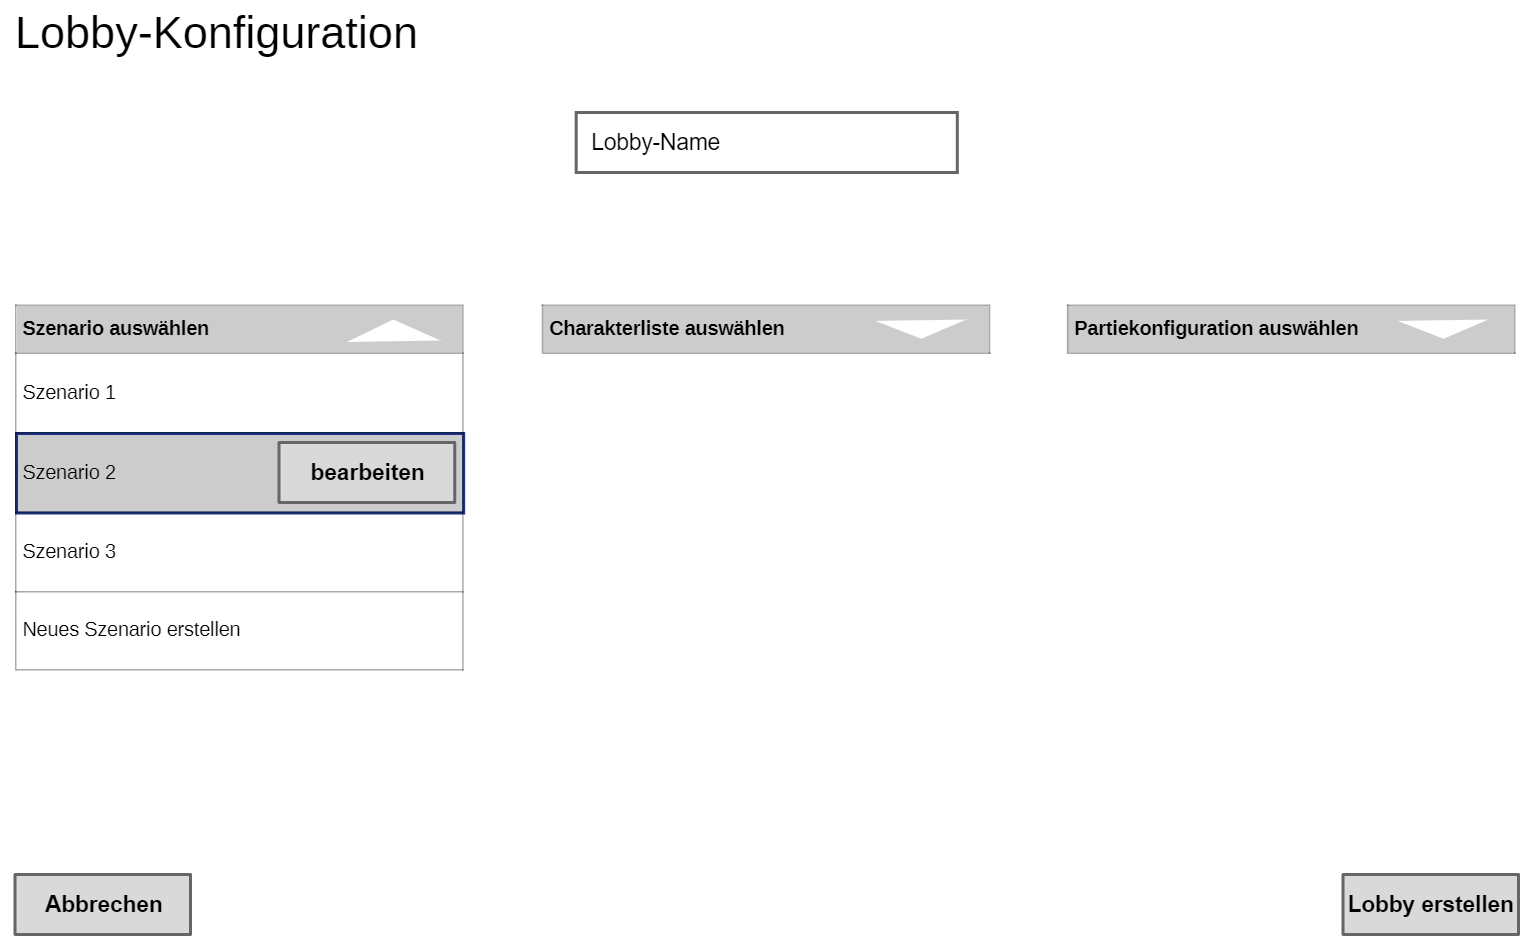
\includegraphics[width=\textwidth]{Meilenstein03/Lobby-Konfiguration_Mockup.png}
  \caption{Mockup für die Lobby-Konfiguration}
\end{figure}

Dialog \glqq{}Lobby\grqq{}

Die Liste mit den verbundenen Clients wird kontinuierlich sortiert, sodass die Spieler immer an oberster Stelle stehen. Die Spieler und die Zuschauer werden untereinander chronologisch nach Beitritt zur Lobby bzw. dem letzten Rollenwechsel sortiert, sodass der Client, der als letzter als Zuschauer der Lobby beigetreten ist bzw. als letzter innerhalb der Lobby die Rolle zu Zuschauer geändert hat, den untersten Eintrag in der Liste hat. Die KI-Clients sind am Benutzernamen erkennbar. 
Mit der Schaltfläche \glqq{}Rolle wechseln\grqq{} ändert sich die eigene Rolle von 'Spieler' zu 'Zuschauer' und umgekehrt. 
Mit der Schaltfläche \glqq{}KI hinzufügen\grqq{} wechselt der Client in den Dialog \glqq{}KI-Konfiguration\grqq{}.
Mit der Schaltfläche \glqq{}Zurück\grqq{} wechselt der Client in den Dialog \glqq{}Lobby-Übersicht\grqq{}.
Die Schaltfläche \glqq{}Bereit\grqq{} ist nur für Clients in der Rolle 'Spieler' eingeblendet. Mit dieser Schaltfläche signalisiert der Benutzer, dass er bereit ist, die Spielpartie zu beginnen. Wenn die Schaltfläche gedrückt wird, wird sie ersetzt durch eine Schaltfläche mit der Aufschrift \glqq{}Nicht mehr bereit\grqq{}. Mit dieser Schaltfläche signalisiert der Benutzer, dass er nun doch nicht mehr bereit ist, die Spielpartie zu beginnen. Die Schaltfläche \glqq{}Spiel starten\grqq{} kann nur dann von einem Client gedrückt werden, wenn dieser Client die Rolle 'Spieler' hat und alle Spieler-Clients der Lobby ihre Spielbereitschaft mit Drücken der Schaltfläche \glqq{}Bereit\grqq{} signalisiert haben.
Mit der Schaltfläche \glqq{}Spiel starten\grqq{} wird eine Spielpartie gestartet und die Ansicht wird zum Dialog \glqq{}Spielfeld\grqq{} gewechselt.

\begin{figure}
  \centering
  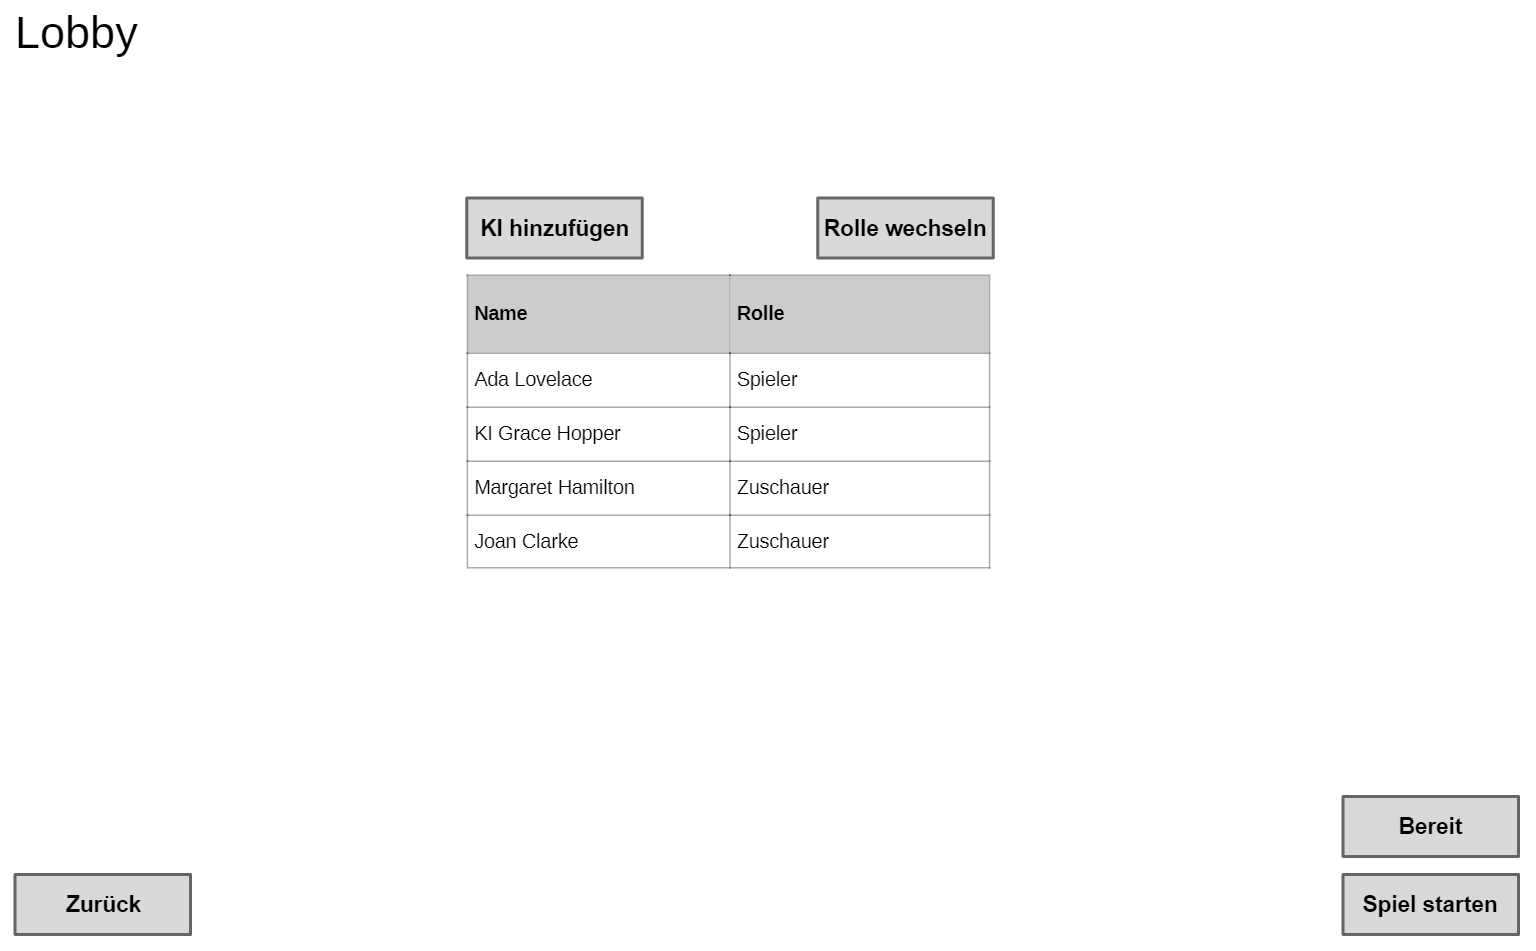
\includegraphics[width=\textwidth]{Meilenstein03/Lobby_Mockup.png}
  \caption{Mockup für das Lobby-View}
\end{figure}

Dialog \glqq{}Szenario-Editor\grqq{}

Alle quadratischen Felder des Spielbretts sind mit Mausklick auswählbar. Die Schaltflächen in Form eines Pluszeichens, die den Rand des Spielbretts säumen erweitern das Spielbrett. Wenn eine Plus-Schaltfläche geklickt wird, dann wird sie ersetzt mit einem neuen Feld und an dessen äußeren Rändern, dem neuen äußeren Rand des Spielbretts erscheinen neue Plus-Schaltflächen. Alle Felder des Spielbretts sind zu Beginn freie Felder. Oberhalb des Spielbretts befinden sich die Icons der verschiedenen Feldarten. Diese lassen sich per Drag-and-Drop auf freie Felder des Spielbretts ziehen. Ist die Szenario-Konfiguration abgeschlossen, kehrt der Benutzer über den Speichern-Button auf die letzte Seite zurück. Über den Abbrechen-Button kehrt der Benutzer auch zur letzten Seite zurück und die Änderungen werden verworfen. Über den Editor-Übersicht-Button gelangt der Benutzer zur Editor-Übersicht. Klickt der Benutzer auf den Abbrechen-Button oder auf den Editor-Übersicht-Button, erscheint eine Warnmeldung, die den Benutzer darauf hinweist, dass nicht gespeicherte Änderungen verworfen werden.

\begin{figure}
  \centering
  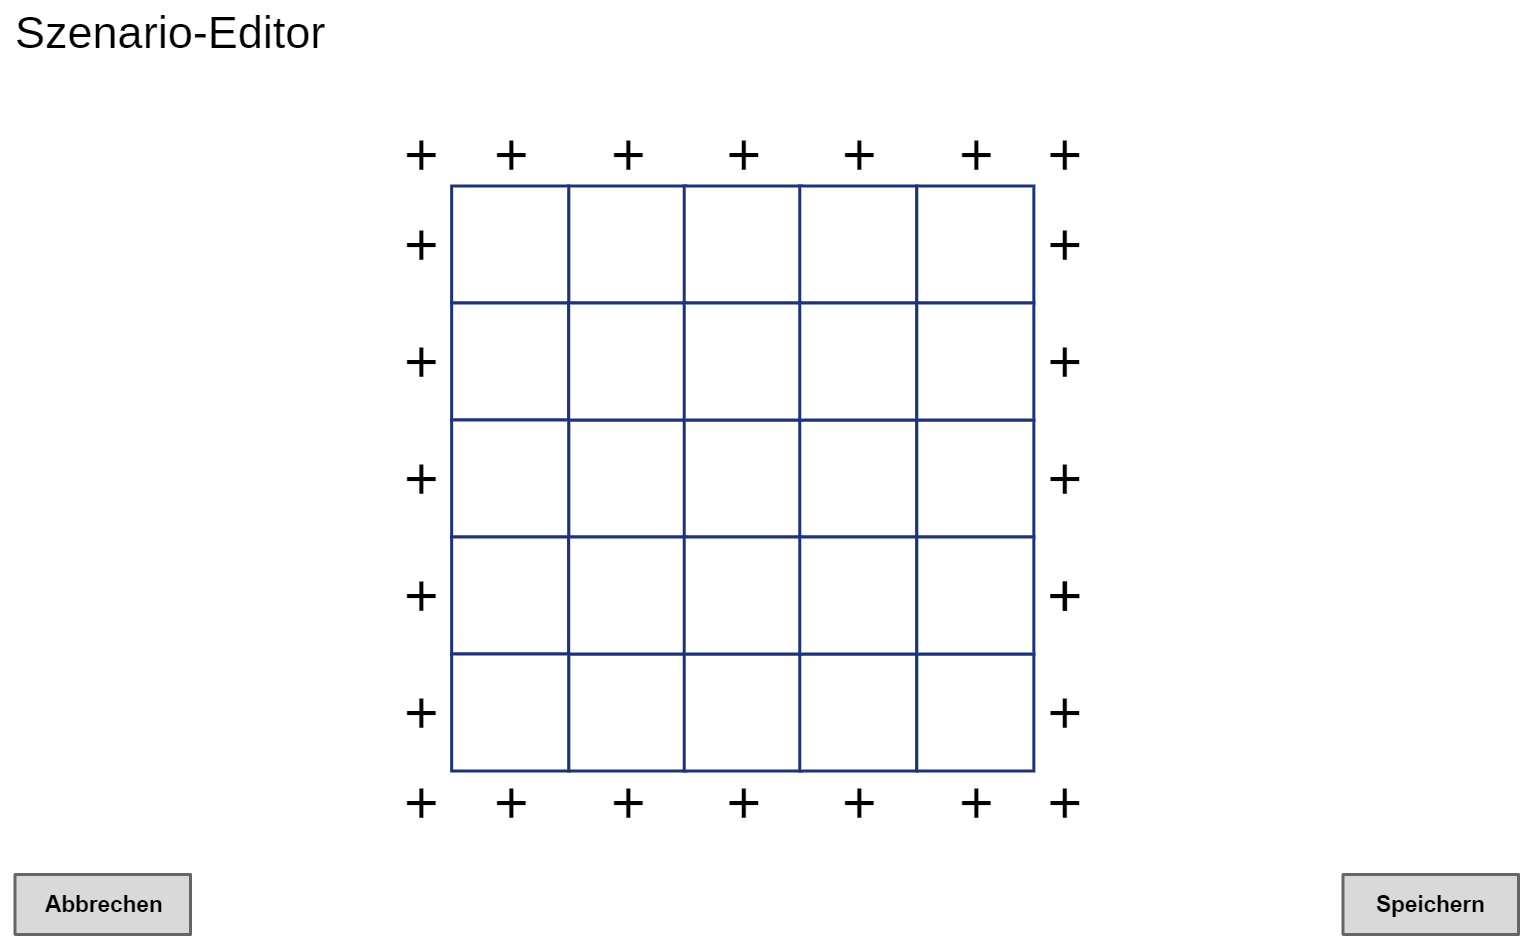
\includegraphics[width=\textwidth]{Meilenstein03/Szenario-Editor_Mockup.png}
  \caption{Mockup für den Szenario-Editor}
\end{figure}

Dialog \glqq{}Charakter-Editor\grqq{}

Dialog \glqq{}Partie-Editor\grqq{}

Mit der Schaltfläche \glqq{}Abbrechen\grqq{} wechselt die Ansicht zu dem Dialog, aus welchem der Partie-Editor aufgerufen wurde. D.h. wenn er aus der Lobby-Konfiguration aufgerufen wurde, dann wechselt die Ansicht zurück zur Lobby-Konfiguration, wenn er aus der Editor-Übersicht geöffnet wurde, dann wechselt die Ansicht wieder dahin zurück.
Mit der Schaltfläche \glqq{}Konfiguration speichern\grqq{} wird die Datei gespeichert und die Ansicht wechselt zu dem Dialog,  aus welchem der Partie-Editor aufgerufen wurde.
Mit der Schaltfläche \glqq{}Editor-Übersicht\grqq{} wird die Ansicht zum Dialog \glqq{}Editor-Übersicht\grqq{} gewechselt, falls alle Änderungen schon gespeichert wurden. Falls noch ungespeicherte Änderungen vorliegen, wird ein Pop-Up-Fenster geöffnet, das abfragt, ob die Konfiguration noch gespeichert werden soll. Wenn in diesem Fenster die Schaltfläche \glqq{}Ja\grqq{} bzw.\glqq{}Nein\grqq{} angeklickt wird, dann wechselt die Ansicht zum Dialog \glqq{}Editor-Übersicht\grqq{} und die Konfiguration wird gespeichert bzw. nicht gespeichert. Mit der Schaltfläche \glqq{}Abbrechen\grqq{} schließt sich das Fenster wieder und der Dialog \glqq{}Partie-Editor\grqq{} wird wieder normal dargestellt.
Mit direkter Eingabe in das Feld der Anzeige des Werts einer Wahrscheinlichkeit oder eines anderen Werts, dem Schieberegler daneben oder den Inkrement- und Dekrementschaltflächen kann der Wert einer Wahrscheinlichkeit in Prozent oder ein Schadens-, Reichweiten-, etc. -wert festgelegt und angepasst werden.

\begin{figure}
  \centering
  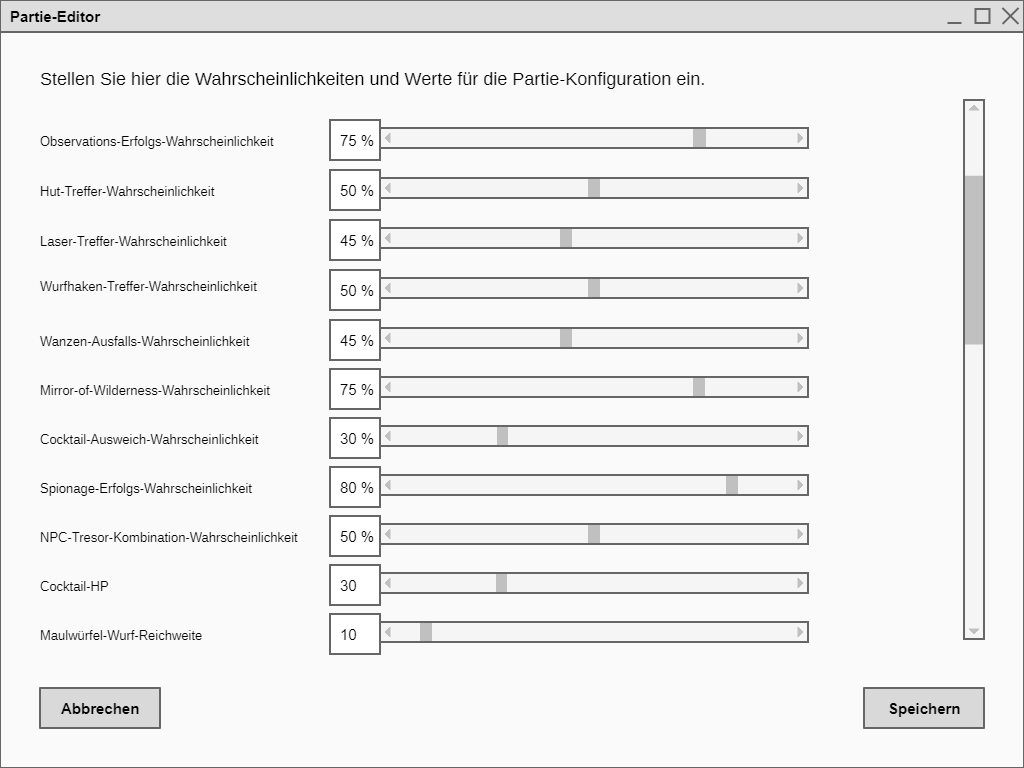
\includegraphics[width=\textwidth]{Meilenstein03/Partie-Editor_Mockup.png}
  \caption{Mockup für den Partie-Editor}
\end{figure}

Dialog \glqq{}KI-Konfiguration\grqq{}

Mit der Schaltfläche \glqq{}Zurück\grqq{} wechselt man zum Dialog \glqq{}Lobby\grqq{}, ohne das ein KI-Client hinzugefügt wurde, mit der Schaltfläche \glqq{}KI hinzufügen\grqq{} wechselt man zum Dialog \glqq{}Lobby\grqq{} und fügt einen KI-Client mit den ausgewählten Parametern hinzu.
Die Intelligenzstufe der KI kann über die Radiobuttons mit den Bezeichnungen 'dumm', 'normal' und 'schlau' eingestellt werden.
Wie in FA-KI 43 beschrieben, muss es möglich sein, die KI mithilfe einer Konfigurationsdatei zu konfigurieren. Deswegen wird in diesem Dialog eine Liste mit Konfigurationsdateien dargestellt, aus denen man eine gespeicherte Konfiguration auswählen kann. Nach der Auswahl einer Konfiguration kann man mit der Schaltfläche \glqq{}Konfiguration laden\grqq{} diese Konfiguration automatisch einstellen.
In das Eingabefeld über der Schaltfläche \glqq{}Konfiguration speichern\grqq{} wird der Name der Konfigurationsdatei vom Benutzer eingetragen. Wenn dort ein valider Dateiname eingegeben wurde, so kann die aktuell eingestellte Konfiguration mit der Schaltfläche \glqq{}Konfiguration speichern\grqq{} in das dafür vorgesehene Verzeichnis gespeichert werden und wird an die Liste der Konfigurationsdateien angefügt.

\begin{figure}
  \centering
  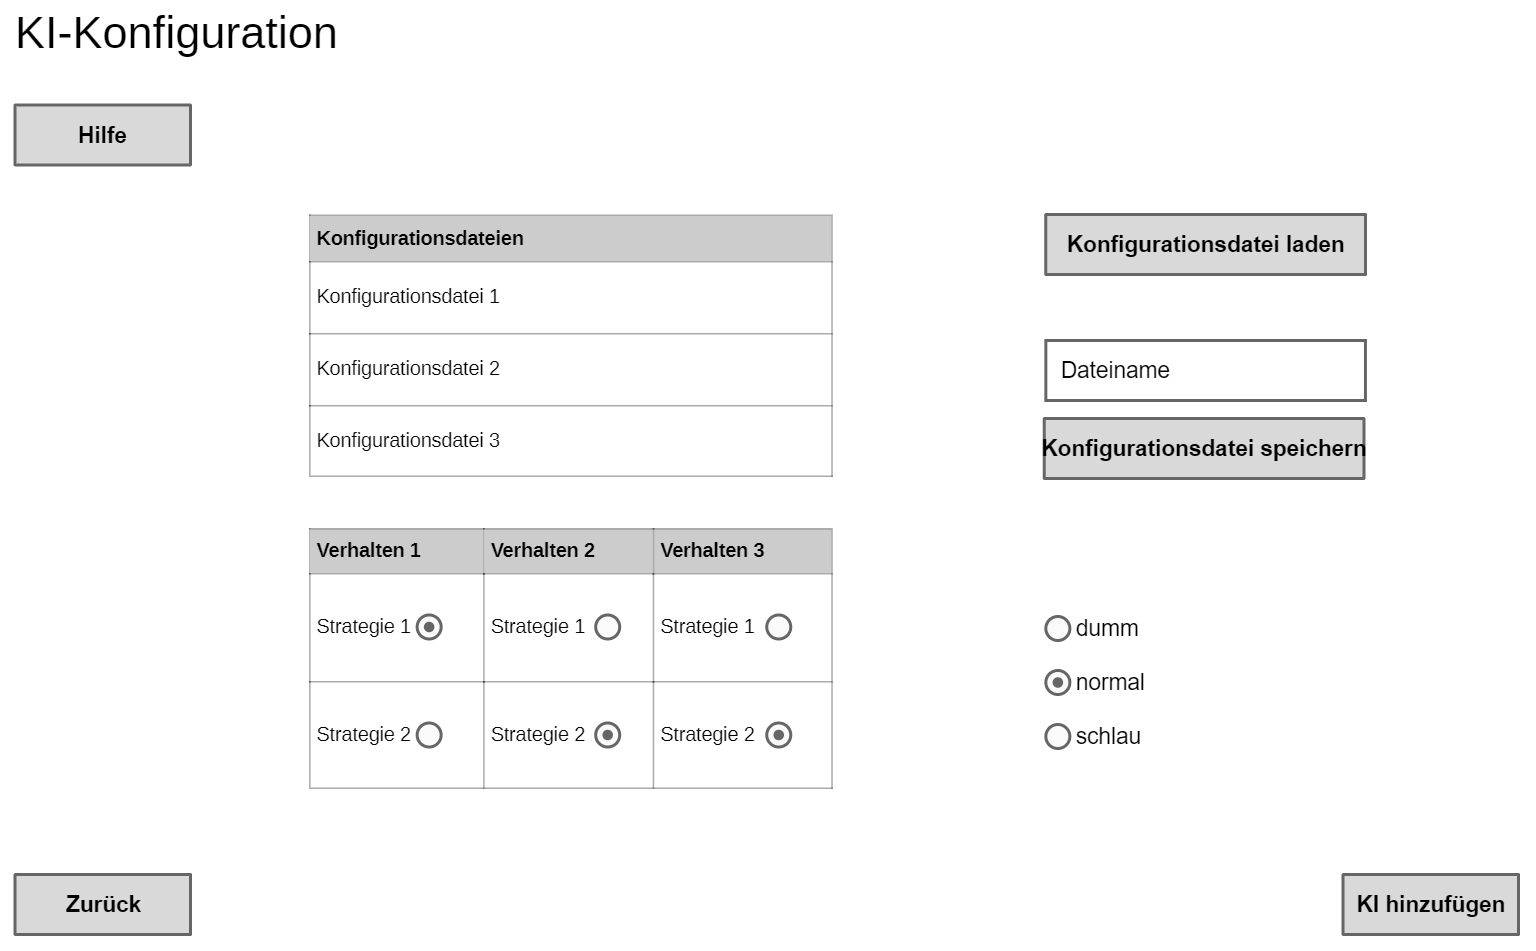
\includegraphics[width=\textwidth]{Meilenstein03/KI-Konfiguration_Mockup.png}
  \caption{Mockup für die KI-Konfiguration}
\end{figure}
\clearpage

\end{document}
